% Monografia para Projeto de Fim de Curso - Exemplo no LaTeX
%-----------------------------------------------------------


%---------------Inicialização de pacotes--------------------

\documentclass[12pt,a4paper,notitlepage,twoside]{book}


\usepackage{graphicx}
\usepackage[utf8]{inputenc}
%\usepackage[latin1]{inputenc} %%pode ser necessário trocar a codificação em sistemas Windows
\usepackage[brazil]{babel}		%%pode ser necessário trocar o pacote de línguas em algumas distribuições LateX
%\usepackage[portuguese]{babel}
\usepackage[T1]{fontenc}
\usepackage{amsmath,amssymb}
\usepackage{amsthm,amsfonts}
\usepackage{color}
\usepackage[colorlinks]{hyperref}
\usepackage{abntex2abrev}
%\usepackage[alf]{abntex2cite} %se você quiser seguir as normas ABNT no sistema autor-data
%\usepackage[num]{abntex2cite} %se você quiser seguir as normas ABNT no sistema numérico
\usepackage{setspace}
\usepackage[toc,page]{appendix}

%Definindo fonte Times (Use os pacotes obsoletos se não conseguir instalar os atualizados)
%\usepackage{times}     %Pacote de fontes obsoleto, apenas texto
%usepackage{mathptmx}  %Pacote de fontes obsoleto, texto e símbolos matemáticos
%\usepackage{newtxtext,newtxmath}  %Pacotes de fontes mais recentes

\usepackage[a4paper,top=30mm,bottom=30mm,inner=30mm,outer=25mm,headheight=7mm,headsep=6mm,footskip=7mm]{geometry}
\usepackage{enumerate}
\usepackage{tabularx}
\usepackage{array} % Necessário para o alinhamento vertical
\usepackage{makecell} % Para controle uniforme da altura das linhas
\usepackage{float}    % Para fixar a tabela no local desejado
\usepackage{subcaption} % Alinhar imagens lado a lado
\usepackage{graphicx} % Reduzir tamanho da fonte de uma equação

\makeindex

%\singlespacing   %%espaçamento simples
%\onehalfspacing
%\setstretch{1.03} %%um pouco melhor que espaçamento simples
\linespread{1.25} %corresponde ao espaçamento 1.5 do MS Word

%---------------Início do documento-------------------------

\begin{document}

\setlength{\extrarowheight}{4pt} % Define uma altura extra para as linhas

\begin{titlepage}
\begin{center}
{\large Universidade Federal de Minas Gerais\\
Escola de Engenharia \\
Curso de Graduação em Engenharia de Controle e Automação\\}

\vspace{6cm}
{\bf\Large Construção, modelagem, projeto de controlador e implementação em hardware para um pêndulo invertido sobre uma esfera\vspace{0.2cm}}
\vspace{4cm}

%\hspace{0.3\textwidth} \parbox{0.65\textwidth}
{\large Samuel Soares do Patrocínio}
\vspace{2cm}  
   
\vspace{2cm}          
%\hspace{0.3\textwidth} 
{\large Orientador: Prof. Fernando de Oliveira Souza}\\
%{\large Supervisor: Eng. Cicrano}

\vfill
%\hspace{0.3\textwidth} 
{\large Belo Horizonte, Novembro de 2024 }
\end{center}

\end{titlepage}

\newpage
\clearpage
\thispagestyle{empty}


\begin{titlepage}

\centering
\textbf{Monografia}\\
\vspace{2cm}
\centering
\textbf{Construção, modelagem, projeto de controlador e implementação em hardware para um pêndulo invertido sobre uma esfera}\\
\vspace{5cm} 

\parbox{1.0\textwidth} 
{\large 
Monografia submetida à banca examinadora
designada pelo Colegiado Didático do Curso de
Graduação em Engenharia de Controle e
Automação da Universidade Federal de Minas
Gerais, como parte dos requisitos para aprovação na
atividade Projeto Final de Curso II.}

\vspace{7cm} 
\centering
Belo Horizonte, Julho de 2014

\end{titlepage}


\pagenumbering{roman}
\addcontentsline{toc}{chapter}{Resumo}

\begin{center}
\huge{{\bf Resumo}}
\vspace{2cm}
\end{center}

No Resumo, em uma única página, em no máximo dois parágrafos, você explicita os seguintes itens: objetivos do projeto e descrição sucinta do local onde ele foi desenvolvido; metodologia utilizada; e resultados alcançados. Leitores experientes decidem se prosseguirão para a leitura do texto completo após lerem o resumo, a conclusão e a introdução. Por isso nestes lugares você deve colocar um esforço maior de convencimento. Além disso, a linguagem utilizada deve ser acessível a leitores com pouca familiaridade com a área, limitando-se o uso de jargões.
 
\begin{sloppypar}
Este novo parágrafo serve para mostrar que ao pular uma ou mais linhas no texto do arquivo .tex, o \TeX\ entende que você está iniciando outro parágrafo. O comando \textsf{sloppypar} força o texto a não ultrapassar as margens. Só deve ser usado se este problema ocorrer.
\end{sloppypar}

 
\clearpage
\thispagestyle{empty}
\cleardoublepage


\addcontentsline{toc}{chapter}{Abstract}

\begin{center}
\huge{{\bf Abstract}}
\vspace{2cm}
\end{center}

Write a version of your ``resumo'' in English. Beware of literal translations and double check the translation of technical terms.
 

 
\clearpage
\thispagestyle{empty}
\cleardoublepage


\addcontentsline{toc}{chapter}{Agradecimentos}

\begin{center}
\huge{{\bf Agradecimentos}}
\vspace{4cm}
\end{center}

Aqui vai o texto dos agradecimentos.
 
\clearpage
\thispagestyle{empty}
\cleardoublepage
\tableofcontents
%\markboth{Conteúdo}{Conteúdo}

\clearpage
%\thispagestyle{empty}
%\cleardoublepage

% Normalmente, este arquivo só contém isto.
\listoffigures
\addcontentsline{toc}{chapter}{Lista de Figuras}
%\markboth{Lista de Figuras}{Lista de Figuras}

\clearpage
%\thispagestyle{empty}
%\cleardoublepage

% Normalmente, este arquivo só contém isto.
\listoftables
\addcontentsline{toc}{chapter}{Lista de Tabelas}
%\markboth{Lista de Tabelas}{Lista de Tabelas}

\clearpage
%\thispagestyle{empty}
%\cleardoublepage

% Normalmente, este arquivo só contém isto.

\pagenumbering{arabic}
\setcounter{page}{1}
\chapter{Introdução}
\label{chap:intro} %este label será usado para referenciar este capítulo

%As primeiras frases têm a missão de prender a atenção do leitor e por isso são as mais importantes do texto. Diga o quanto antes o que você fez e quais são os resultados alcançados. Ao terminar de ler a introdução o leitor tomará uma nova decisão de se vale a pena ou não continuar lendo o texto. Capte a atenção do leitor bem aqui.

%A comunicação escrita é considerada umas das cinco habilidades mais importantes por profissionais de engenharia e um engenheiro passa em média mais de $25$\% do seu tempo escrevendo \cite{eggert2002response,spretnak1982survey}. Uma quantidade similar de tempo é gasta na escrita de correspondência e de relatórios técnicos \cite{cunningham2012perceptions}. Dessa forma, encare a escrita do seu projeto como um treinamento nessa importante habilidade.

%Neste texto você encontrará não apenas uma estrutura para escrever seu trabalho em \LaTeX, mas também um pequeno manual de boas práticas na escrita técnica. Leia com atenção e coloque as sugestões em prática à medida que preenche o texto com o conteúdo do seu próprio projeto. Também será apresentado um número de vícios de escrita comumente encontrados nas monografias de alunos. 

%A seguir está a estrutura de organização sugerida pelo colegiado do curso. Note que ela não é necessariamente a melhor para contar a história do seu projeto. Você pode por exemplo preferir usar títulos mais pertinentes ao seu contexto. Contudo, o seu texto deve conter cada um dos pontos a seguir.

\section{Motivação e Justificativa}
\label{sec:motivacao}

O avanço contínuo na área de controle e automação exige que os futuros engenheiros dominem técnicas práticas e teóricas para solucionar problemas reais de engenharia. No contexto do curso de Engenharia de Controle e Automação, é essencial que os alunos tenham acesso a plataformas de aprendizagem que unam teoria e prática de maneira dinâmica e interativa. Nesse cenário, o desenvolvimento de sistemas experimentais versáteis e acessíveis é uma abordagem eficiente para consolidar o aprendizado e despertar o interesse por sistemas de controle complexos.

O projeto proposto consiste na construção de um robô que se equilibra sobre uma esfera, uma aplicação concreta do conceito de pêndulo invertido. Esse sistema é amplamente utilizado no ensino de técnicas de controle devido à sua natureza desafiadora e suas características dinâmicas, que exigem uma compreensão aprofundada de modelagem, análise e implementação de controladores.

A utilização de modelagem 3D e impressão em impressoras 3D para a construção do robô garante um custo reduzido, acessível tanto para o laboratório quanto para alunos interessados em replicar o projeto. Essa abordagem também assegura que eventuais danos à planta possam ser facilmente reparados, incentivando o uso contínuo e livre do sistema pelos discentes. Dessa forma, o projeto atende a dois objetivos principais: a oferta de um sistema dinâmico e interessante para o estudo de controle e a promoção de um ambiente de aprendizagem prático e sustentável.

%Argumente sobre a importância do projeto desenvolvido usando uma visão de alto nível, sem entrar em detalhes. Contextualize seu projeto dentro do local de execução ou da literatura e explique como ele é necessário ou inovador. É possível fazer uma breve revisão bibliográfica, confrontando seu trabalho com outras referências bibliográficas para mostrar a sua contribuição. No quesito contribuição, é muito importante deixar claro o tempo todo que partes do projetos foram executadas por outros e que partes foram executadas por você. Caso contrário, corre-se o risco de inadvertidademente tomar crédito pelo trabalho de outrem, o que pode ter implicações legais. 

\section{Objetivos do Projeto}
\label{sec:objetivos}

Tendo em vista o exposto acima, este projeto tem por objetivos:

\begin{enumerate}[a)]
\item  Projetar e construir um robô do tipo pêndulo invertido que se equilibra sobre uma esfera, utilizando conceitos aprendidos ao longo do curso de Engenharia de Controle e Automação;
\item Tornar a construção viável e replicável por meio da utilização de impressão 3D, proporcionando durabilidade e acessibilidade; 
\item Implementar e validar técnicas de controle avançadas para garantir a estabilidade do sistema e seu funcionamento eficiente.

Esses objetivos foram estabelecidos com a finalidade de integrar o conhecimento teórico adquirido ao longo do curso com aplicações práticas relevantes, contribuindo para a formação de engenheiros mais preparados para lidar com desafios reais.
\end{enumerate}

%O conteúdo desta seção pode se sobrepor um pouco com o da seção anterior, podendo ela ser um sumário dos pontos expostos anteriormente. A escolha do título da seção talvez seja mais apropriada para a fase de proposta do projeto. Afinal, nesta fase se conhecem os objetivos e não os resultados. Por outro lado, fará pouco sentido discutir objetivos quando o projeto está finalizado, especialmente se tais objetivos não foram alcançados. 


\section{Local de Realização}
\label{sec:empresa}

O desenvolvimento do projeto será realizado no Laboratório de Controle da Escola de Engenharia da Universidade Federal de Minas Gerais (UFMG). A impressão das peças será viabilizada por meio de uma impressora 3D disponibilizada pelo professor Fernando de Oliveira Souza, que também supervisionará as etapas práticas e fornecerá o suporte técnico necessário.


\section{Estrutura da Monografia}
\label{sec:organizacao}

Esta monografia está organizada em quatro capítulos, além desta introdução. O Capítulo 1 apresenta uma visão geral do projeto, incluindo sua motivação, objetivos e local de execução. O Capítulo 2 explora os princípios fundamentais relacionados ao pêndulo invertido, detalhando conceitos essenciais para o entendimento do sistema e do controle aplicado. O Capítulo 3 descreve a metodologia adotada no projeto, abrangendo as etapas de modelagem 3D, construção da planta física, modelagem matemática e projeto dos controladores. Por fim, o Capítulo 4 apresenta as conclusões obtidas, as contribuições do projeto e sugestões para trabalhos futuros, além de relatar os principais desafios enfrentados.


\clearpage
\chapter[Descrição do Processo]{Descrição do Problema/Processo ou O Processo de Fazer Alguma Coisa}
\label{chap:descricaoproblema}
%Note que, como nome do capítulo é muito longo, fornecemos um nome abreviado uso no cabeçalho

Se desejar, uma visão geral do capítulo pode ser colocada antes da primeira seção. Este é o capítulo de descrição do processo e formulação do problema. Tendo em vista que se trata de uma monografia de engenharia de controle e automação, em muitos casos será fundamental a apresentação dos sensores e atuadores do processo.


\section{Processo de Fazer Alguma Coisa}
\label{sec:hist}

Cada seção inicia pela descrição do seu conteúdo e pode terminar com um parágrafo de conexão com a seção seguinte. 

Antes de formular o problema, \textbf{não se esqueça de fazer todas as definições necessárias}. Também devem-se detalhar os aspectos complementares da abordagem: se estamos estudando um aspeto particular do problema, se a resposta encontrada é universal ou dependente de simplificações e hipóteses prévias.


\section{Instrumentação do Processo}
\label{sec:instrumentação}

Descreva a aparelhagem e o equipamento utilizados bem como a ligação entre os diversos componentes. Nesta seção e, ao longo de todo o texto, você deve dar detalhes suficientes para que qualquer pessoa consiga reproduzir seus experimentos.

Contudo, \textbf{não disperse o leitor com detalhes irrelevantes} ou aspectos
demasiado técnicos ou formais. Reserve tais detalhes para um
apêndice.

Como uma imagem vale mais que mil palavras, e como usar mil palavras prejudicaria a clareza do texto, ilustramos o processo com a Figura \ref{fig:processo}. Lembrar que toda figura deve ser comentada no texto, você nunca deve colocar figuras que fiquem ``soltas'' no texto.  

\begin{figure}[thpb]
  \centering
  \resizebox{120mm}{!}{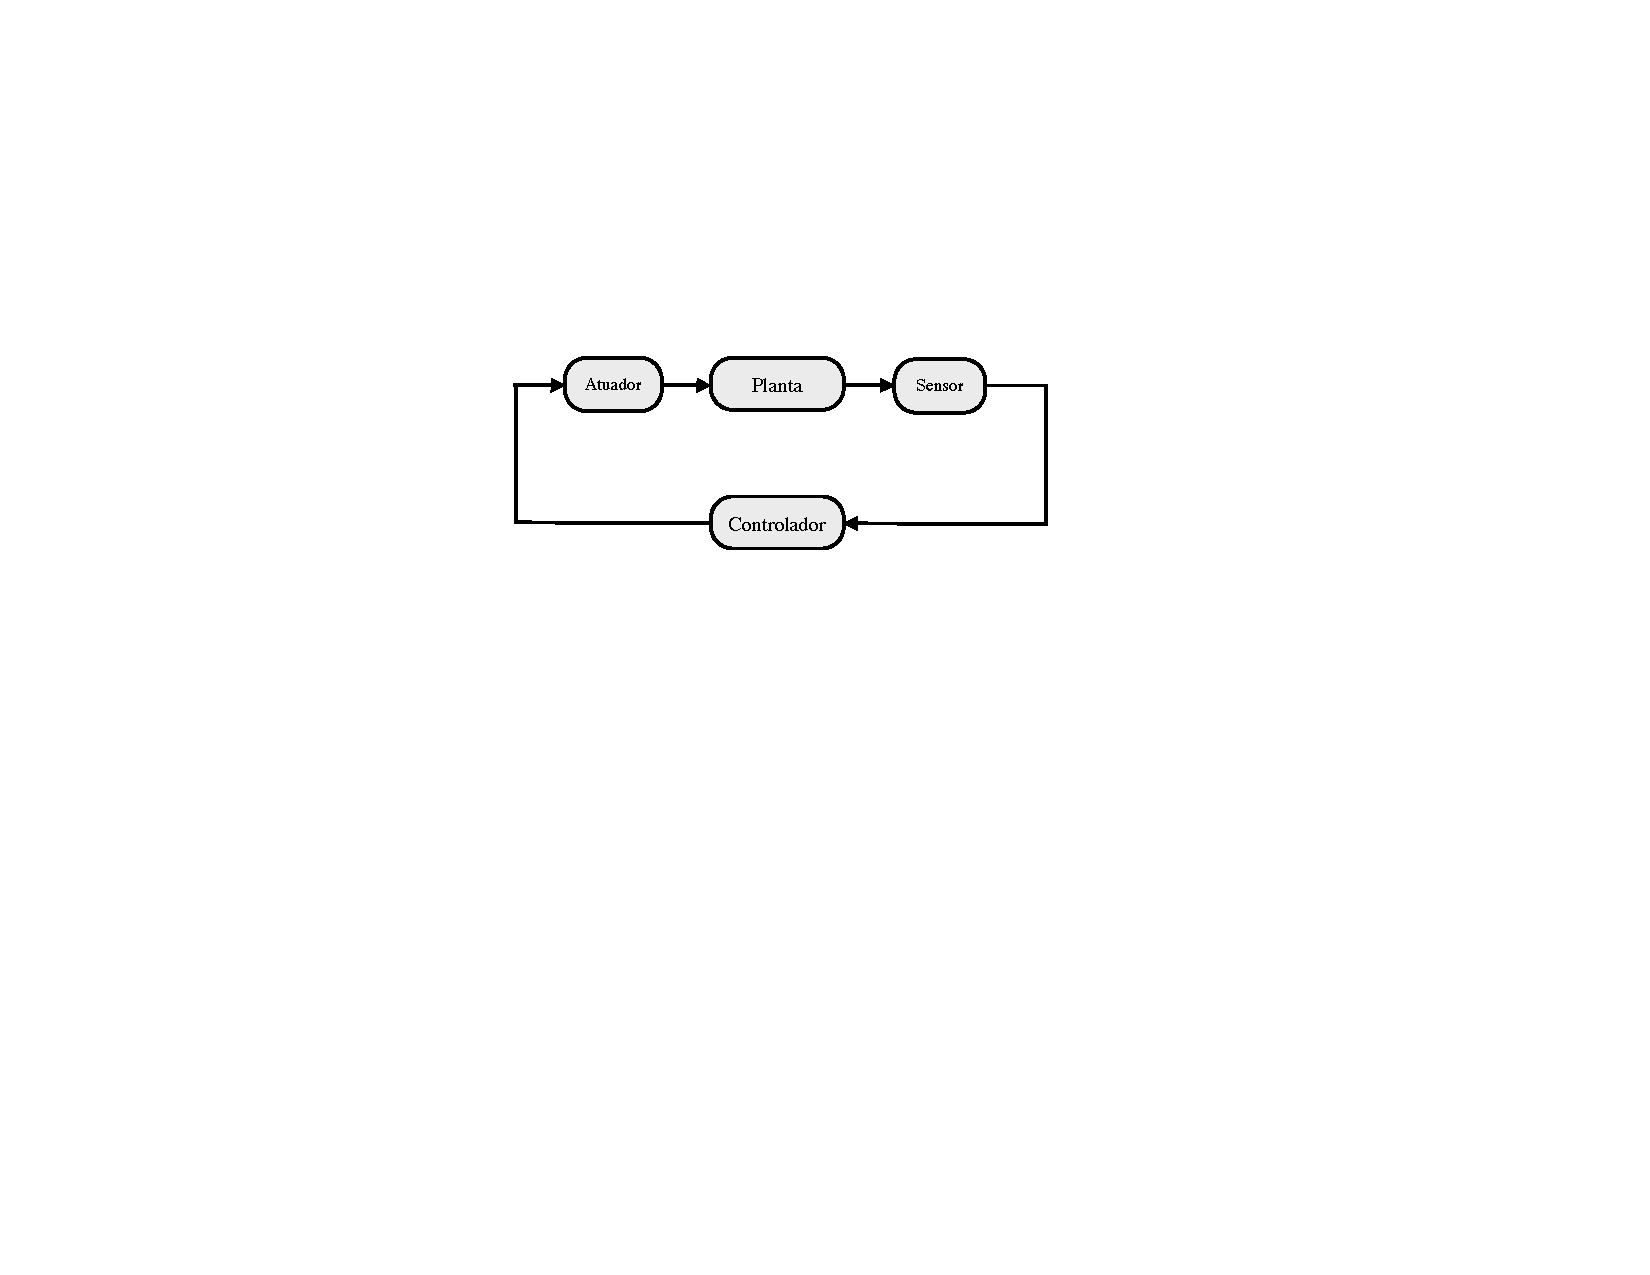
\includegraphics{DescricaoProcesso/Figuras/FiguraProcesso.pdf}}
  \caption{Aqui escrevemos \textbf{toda} informação pertinente à figura. Ou seja, este texto deve ser uma descrição auto-contida da figura, não sendo necessário recorrer ao corpo de texto para saber detalhes sobre a mesma. \emph{Fonte:} Citar fonte se figura 	não for elaborada pelo autor e \textbf{pedir permissão para usar!}}
  \label{fig:processo}
\end{figure}


\section{Situação Atual/Estado da Arte/Revisão da Literatura}
\label{sec:revisão}

Este é o espaço para uma revisão detalhada do enquadramento do problema. Isso inclui descrever a situação atual do processo, aquilo que foi feito até então dentro da empresa/laboratório, e aquilo que se pode chamar de ``Estado da Arte'', ou seja, uma apresentação do conhecimento preexistente
sobre o tema do projeto.

A elaboração desta seção tipicamente demanda uma boa revisão da literatura. Deve haver, quando aplicável uma análise das soluções potencialmente concorrentes, elencando vantagens e desvantagens.

\subsection{Como Elaborar uma Revisão da Literatura}

Ao selecionar referências, devem-se preferir referências de veículos confiáveis, que tenham por exemplo processo de revisão por pares. Portanto, dá-se preferência a artigos em periódicos e livros, em seguida teses e dissertações, artigos em anais de congresso e por fim relatórios. Evitar citar páginas da internet por oferecem menor garantia da informação nelas contida. 

Pesquise sua bibliografia em bases confiáveis como o \textsf{Web of Science}, \textsf{Scopus}, ou o \textsf{Google Scholar}. \textbf{Não use uma ferramenta de busca comum!} (elas não foram feitas pensando no \emph{ranking} de textos científicos) Use o número de citações de uma dada referência como um indicador de sua qualidade. Explore os artigos que citam a referência estudada bem como os artigos que ela cita.

Prefira as referências mais recentes quando se tratar de um assunto na fronteira do conhecimento ou de tecnologia de ponta. Quando se tratar de um assunto já consolidado, prefira citar livros ou artigos com muitas citações. 

Evite citar informações de segunda-mão e procure na medida do possível rastrear a fonte original. Contudo, em situações em que a fonte original é de acesso mais difícil, seja por ter tido publicação limitada como no caso de relatórios ou por não ser em língua inglesa ou portuguesa, é preferível a citação de segunda-mão em um veículo mais acessível.

Para gerenciar suas referências, use uma ferramenta de software como o \textsf{Mendeley}, que permite gerar arquivos .bib para uso em {\LaTeX} ou simplesmente gerar a lista de referências para uso direto em editores de texto. Em \LaTeX, mais especificamente Bib\TeX, a lista de referências é criada a partir de um arquivo .bib, que é uma espécie de banco de informações bibliográficas em que cada entrada é uma referência associada a uma chave para citação. A lista criada incluirá apenas as referências citadas ao longo do texto, mesmo que haja mais referências no arquivo .bib. As informações bibliográficas no formato Bib\TeX também podem ser obtidas para cada referência em ferramentas como o \textsf{Google Scholar} e então coladas no arquivo .bib.

Na Seção \ref{sec:comocitar} discutiremos como e quando as citações devem ser usadas.

\section{Resumo do Capítulo}

Tente não terminar de forma abrupta. Se for escrever algo aqui, não seja genérico!


\clearpage

\chapter{Metodologia}
\label{chap:metodologia}

\section{A modelagem 3D}
\label{sec:modelagem3d}

Para a realização da modelagem matemática, primeiro foi feito um modelo 3D do robô no software OnShape. As peças modeladas formam o corpo do robô. As rodas, os motores e a esfera não foram impressos em 3D, mas são representados no modelo, como é mostrado na imagem a seguir:

\begin{figure}[H]
    \centering
    \begin{subfigure}[b]{1.0\textwidth}
        \centering
        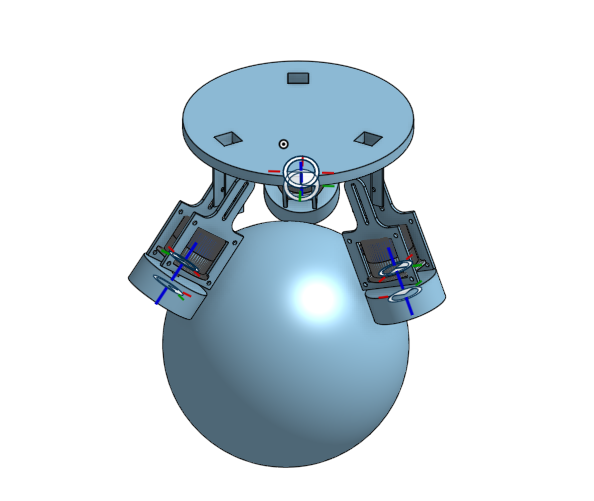
\includegraphics[width=\linewidth]{Metodologia/Figuras/ballbot.png}
        \caption{Modelo 3D}
        \label{fig:modelo_3D}
    \end{subfigure}
\end{figure}

O corpo do robô é um pequeno cilindro, onde são fixados os componentes eletrônicos. Além disso, possui partes que podem se mover para variar o ângulo das rodas e facilitar a acomodação. Essas partes também envolvem a fixação dos motores ao corpo.

\section{A modelagem matemática}
\label{sec:modelagemmatematica}

Para o projeto de controle, fez-se necessário realizar a modelagem mecânica do robô. A etapa seguinte relata como isso foi feito por meio da separação em planos 2D e obtenção das equações de movimento pelo cálculo do Lagrangiano e aplicação das equações de Euler-Lagrange. O passo a passo para realizar os cálculos foi semelhante ao presente no artigo \cite{phdthesis} e adaptado ao modelo projetado.

\subsection{Descrição do modelo}

O robô projetado foi um sistema tridimensional complexo formado por uma esfera, três rodas omnidirecionais e um corpo. Para a representação matemática simplificada, esse modelo foi dividido em três modelos planos independentes (Fig: \ref{fig:modelos_planos}).

\begin{figure}[H]
    \centering
    \begin{subfigure}[b]{0.4\textwidth}
        \centering
        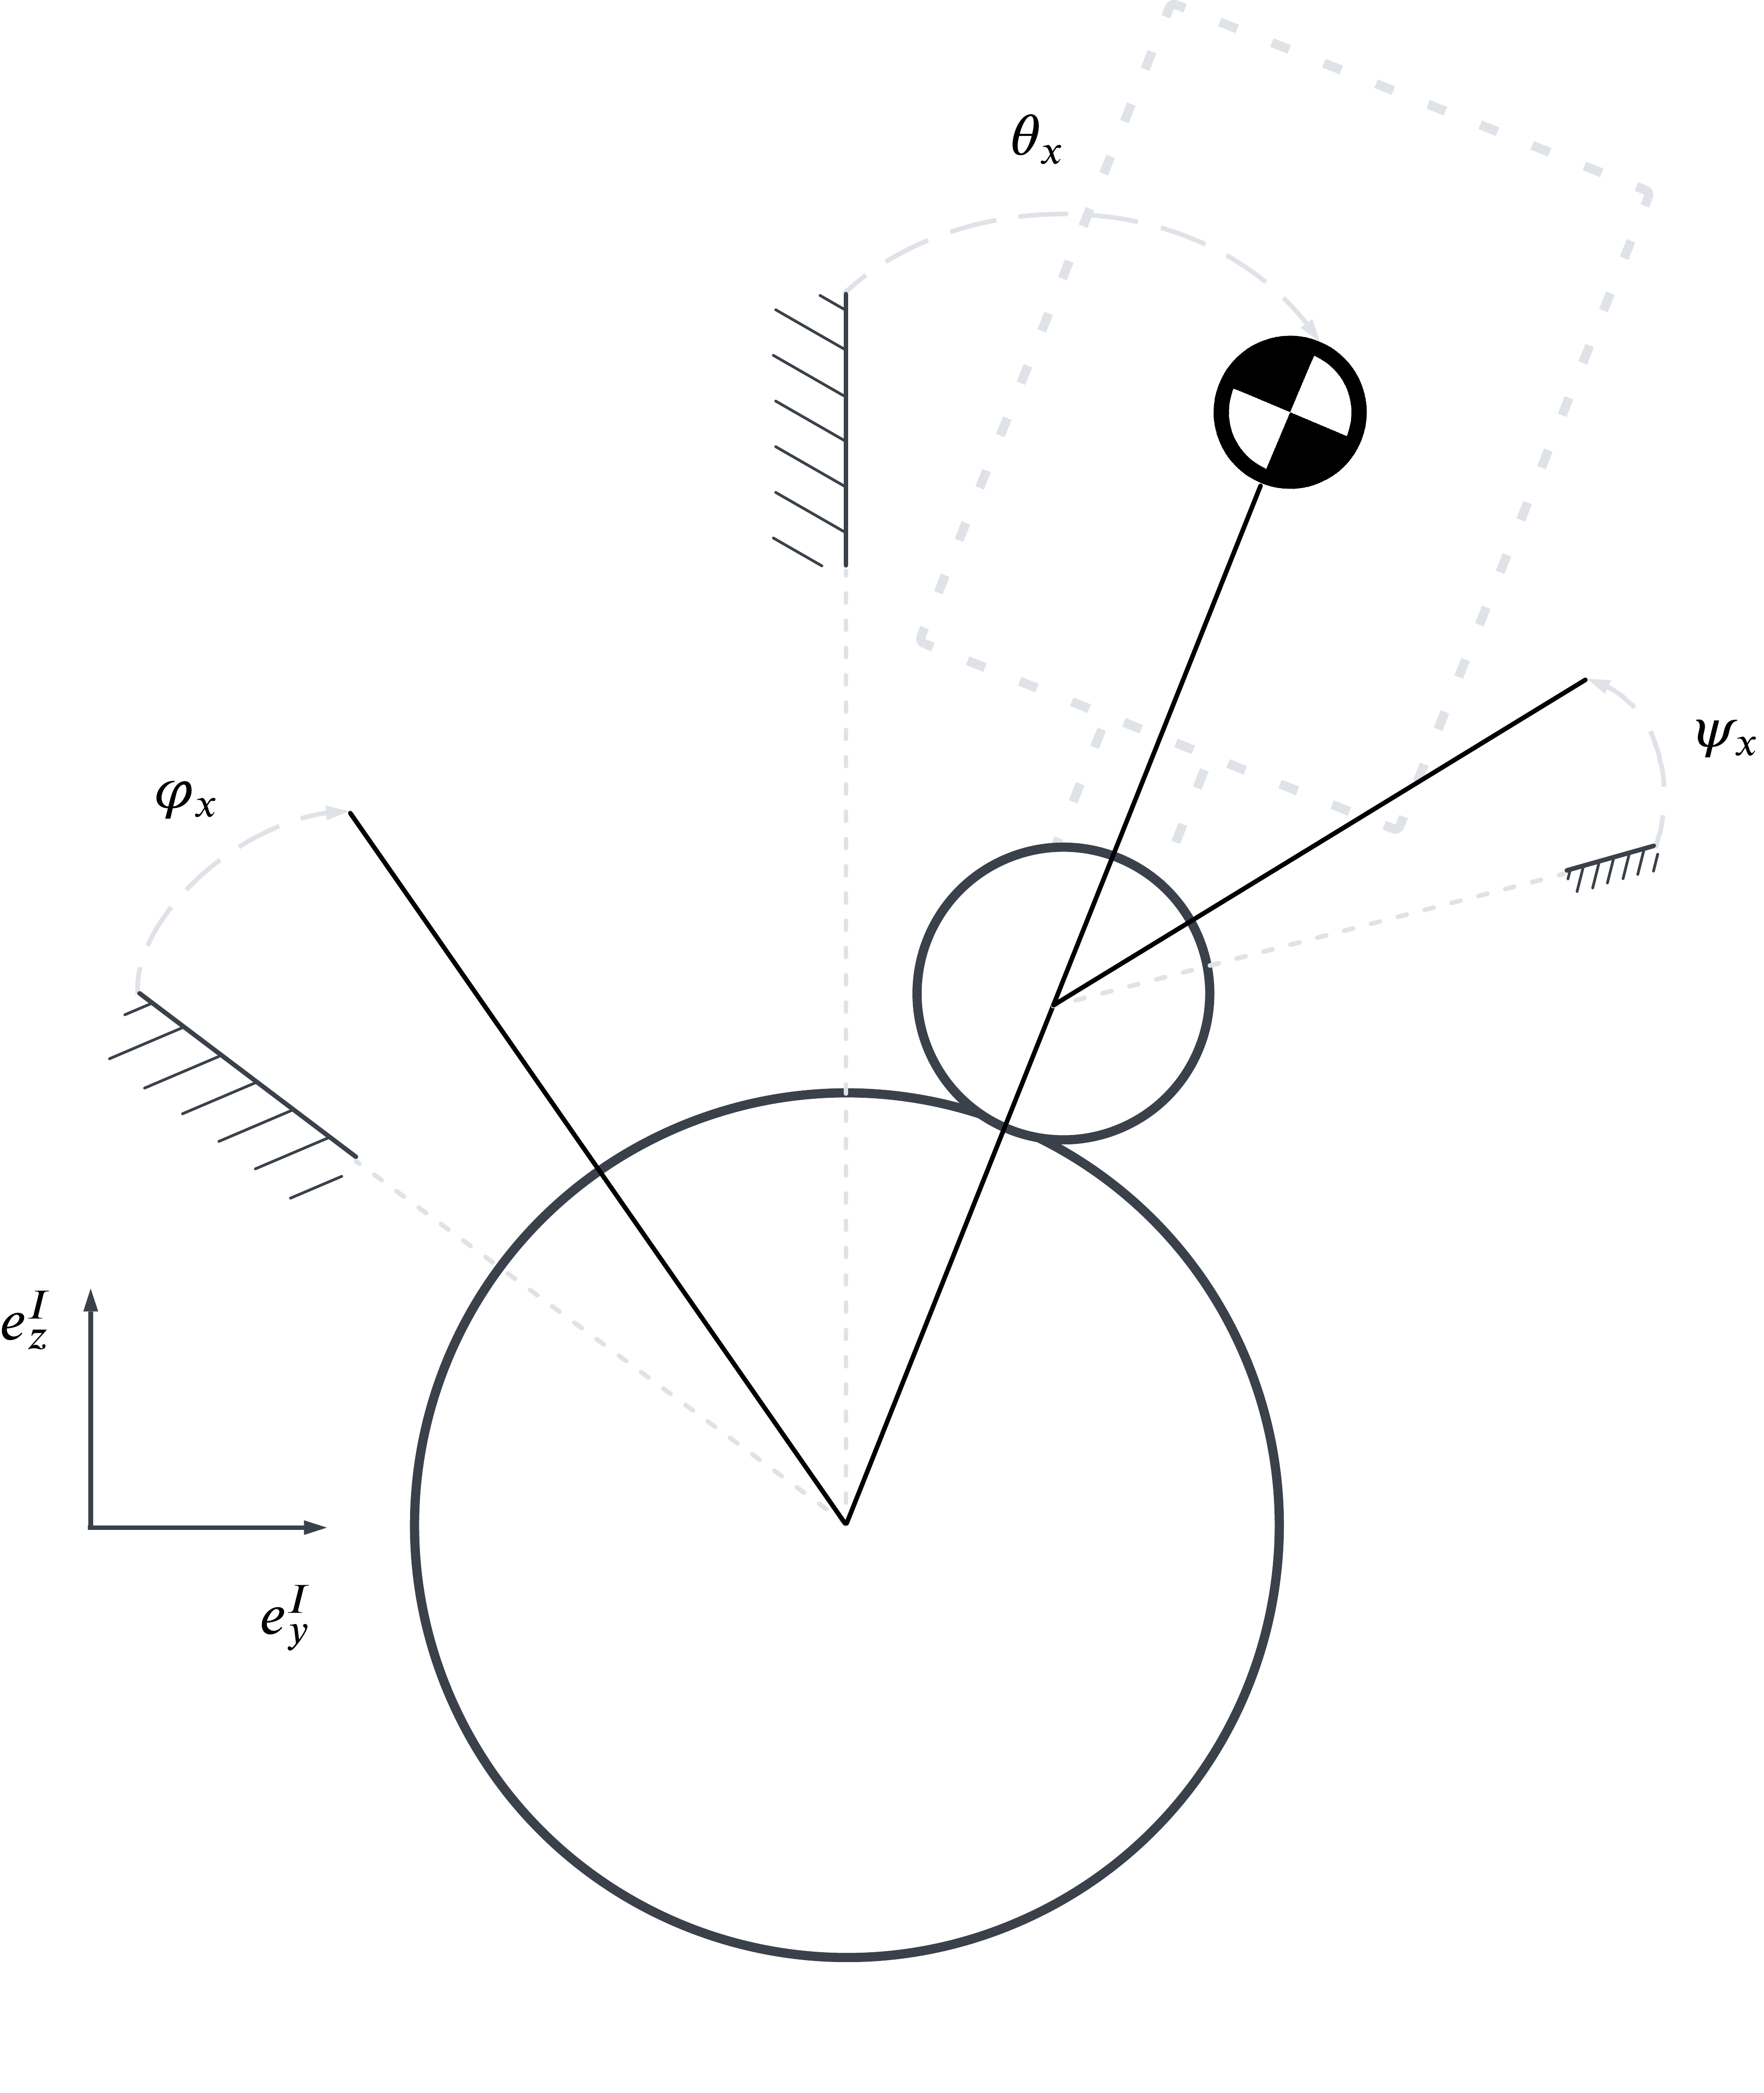
\includegraphics[width=\linewidth]{Metodologia/Figuras/modelo_plano_yz.png}
        \caption{Modelo no plano y-z}
        \label{fig:modelo_yz}
    \end{subfigure}
    \hfill
    \begin{subfigure}[b]{0.4\textwidth}
        \centering
        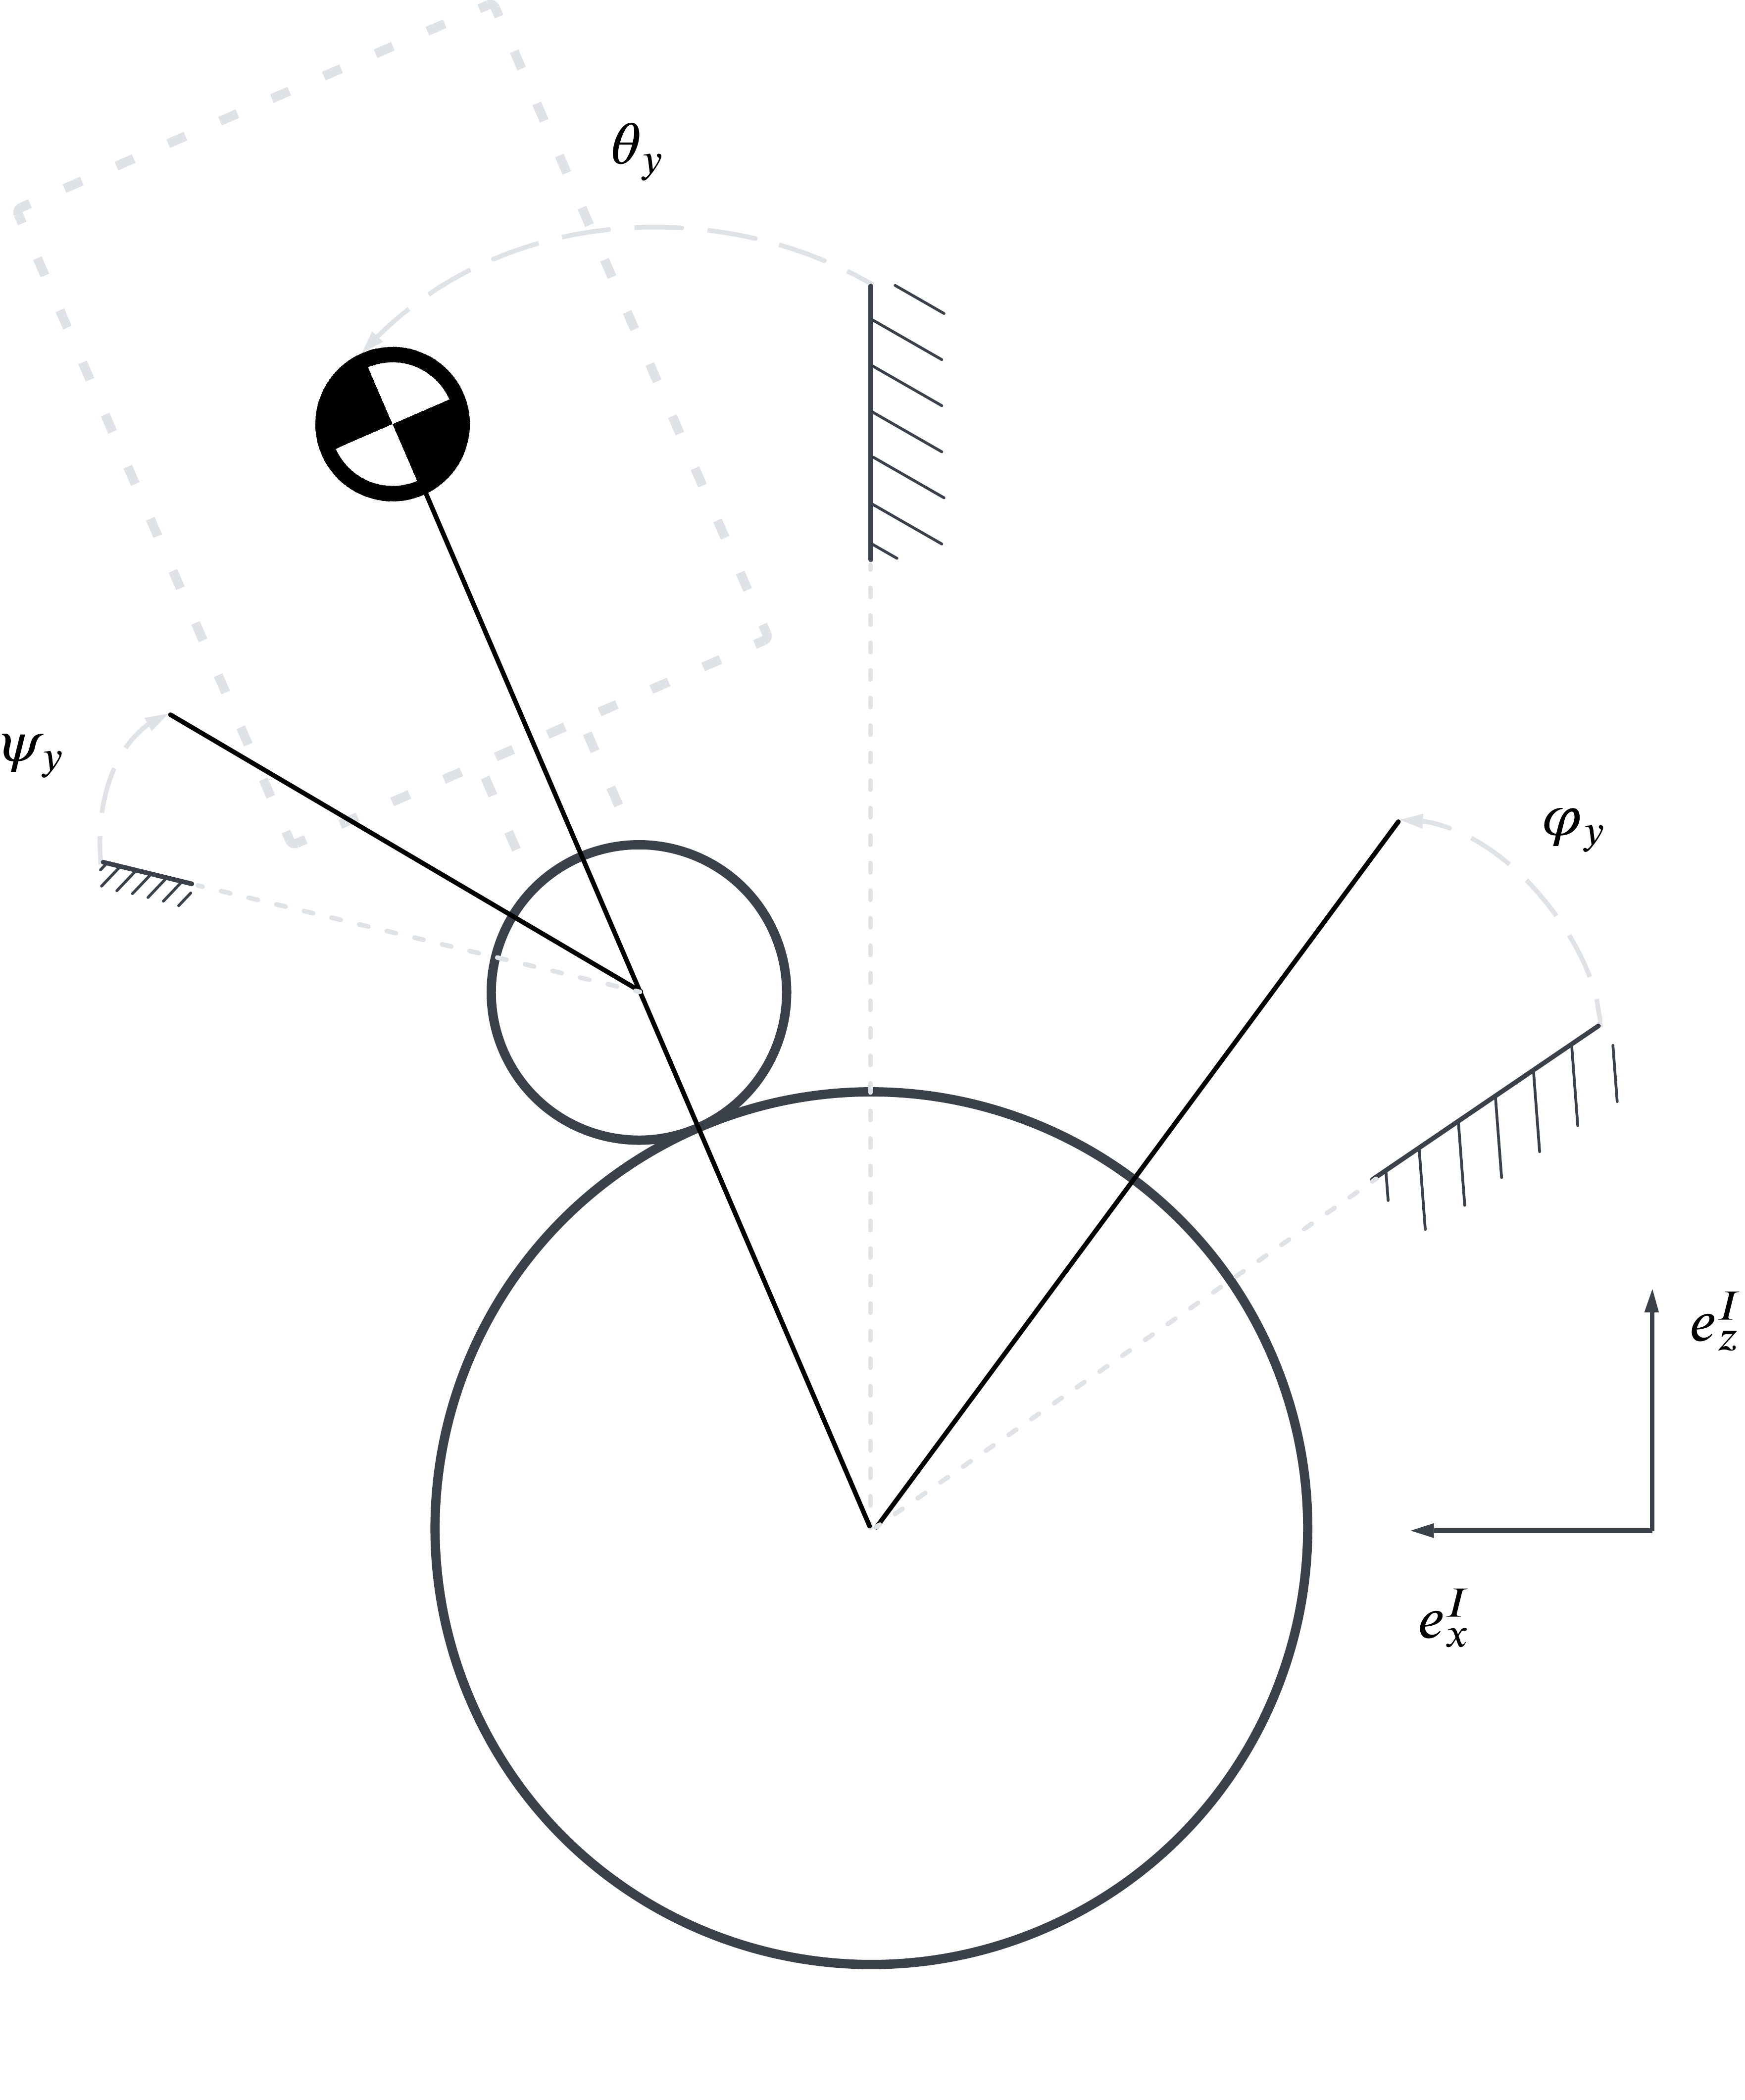
\includegraphics[width=\linewidth]{Metodologia/Figuras/modelo_plano_xz.png}
        \caption{Modelo no plano x-z}
        \label{fig:modelo_xz}
    \end{subfigure}
    \hfill
    \begin{subfigure}[b]{0.4\textwidth}
        \centering
        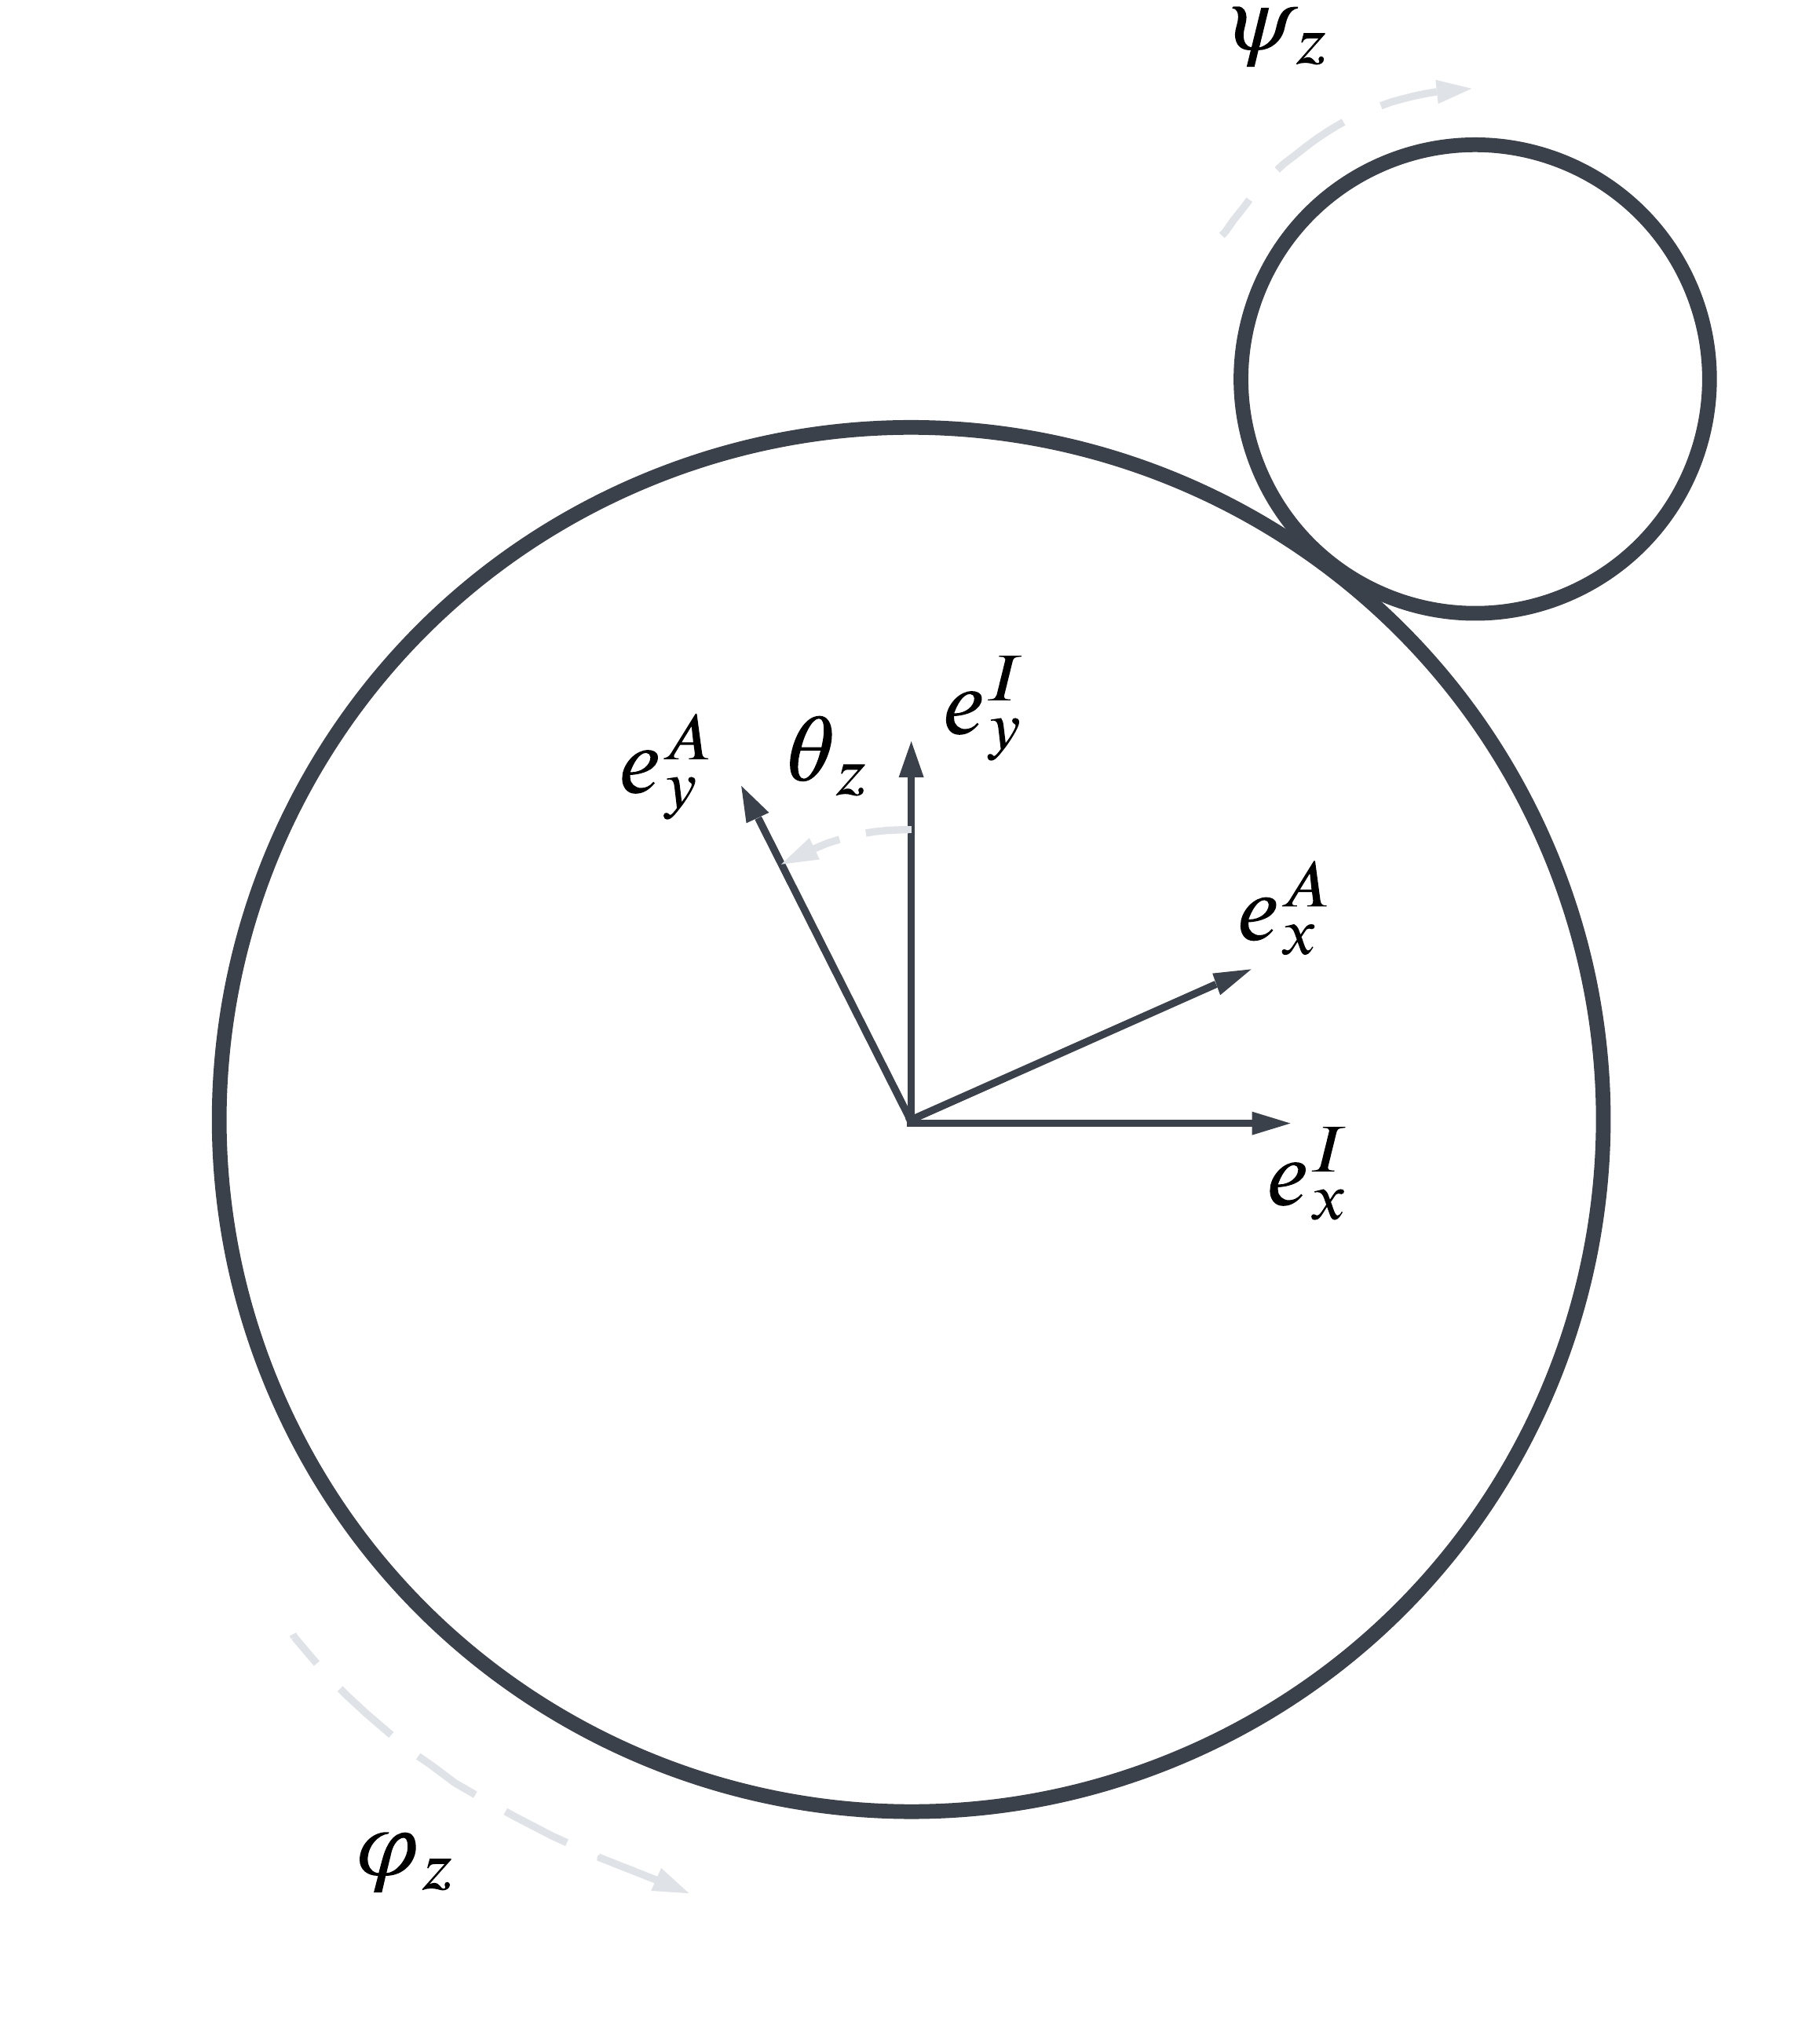
\includegraphics[width=\linewidth]{Metodologia/Figuras/modelo_plano_xy.png}
        \caption{Modelo no plano x-y}
        \label{fig:modelo_xy}
    \end{subfigure}
    \caption{Modelos nos diferentes planos}
    \label{fig:modelos_planos}
\end{figure}

Dessa forma, as três rodas omnidirecionais, que tinham o papel de movimentar o robô, foram transformadas em rodas virtuais, e cada uma foi representada em um modelo. Por causa dessa simplificação, posteriormente foram feitos cálculos para a conversão de posições e velocidades das rodas virtuais para as rodas reais.

\subsection{Suposições}

Os três modelos foram gerados a partir da subdivisão em planos do modelo tridimensional. Consequentemente, os efeitos de acoplamento entre eles foram desconsiderados. Nesse contexto, assumiu-se que o modelo representado no plano $y$-$z$ e o modelo representado no plano $x$-$z$ eram figuras espelhadas uma da outra. Por outro lado, o terceiro modelo, representado no plano $x$-$y$, tinha uma visão única, e apenas descrevia a rotação em torno do eixo \( z \) no sistema de coordenadas fixo do corpo (Fig: \ref{fig:modelo_xy}).

Ademais, com o intuito de simplificar ainda mais os cálculos e garantir a viabilidade do modelo matemático, foram adotadas as seguintes suposições:

\begin{itemize}
    \item Não há deslizamento entre a esfera e a superfície em que o robô está posicionado, assim como entre a esfera e as rodas omnidirecionais.
    \item Apenas o atrito em torno do eixo $z$, entre a esfera e a superfície, foi considerado. Todas as demais forças de atrito foram desconsideradas por serem consideradas irrelevantes.
    \item As interações entre os pontos de contato do robô são idealizadas, ou seja, não há deformações em nenhum desses pontos.
    \item A dinâmica dos motores é significativamente mais rápida do que a dinâmica de estabilização do robô, permitindo que a primeira seja tratada como praticamente instantânea em relação à segunda.
    \item A esfera está restrita a movimentos no plano horizontal, eliminando quaisquer componentes verticais.
\end{itemize}

\subsection{Parâmetros}

O robô possui alguns parâmetros estruturais que foram medidos e estão dispostos na tabela a seguir:

\begin{table}[H]
\centering
\begin{tabular}{|m{6cm}|c|c|c|}
\hline
Parâmetro & Símbolo  & Valor & Unidade de medida \\ \hline
Massa da esfera & $m_K$  & - & $kg$ \\ \hline
Massa da roda & $m_W$  & - & $kg$ \\ \hline
Massa do corpo & $m_A$  & - & $kg$ \\ \hline
Raio da esfera & $r_K$  & - & $m$ \\ \hline
Raio da roda & $r_W$  & - & $m$ \\ \hline
Distância entre o centro da esfera e o centro de massa do corpo & $l$ & - & $m$ \\ \hline
Momento de inércia da esfera & $\Theta_K$  & - & $kg \cdot m^2$ \\ \hline
Momento de inércia da roda nos planos $x$-$z$ e $y$-$z$ & $\Theta_W$  & - & $kg \cdot m^2$ \\ \hline
Momento de inércia da roda no plano $x$-$y$ & $\Theta_{W,xy}$  & - & $kg \cdot m^2$ \\ \hline
Momento de inércia do corpo & $\Theta_{A}$  & - & $kg \cdot m^2$ \\ \hline
Momento de inércia do corpo no plano $x$-$y$ & $\Theta_{A,xy}$  & - & $kg \cdot m^2$ \\ \hline
Ângulo entre o ponto de contato das rodas e o eixo z do sistema de coordenadas da esfera & $\alpha$  & - & $graus$ \\ \hline
Aceleração da gravidade & $g$  & $9,8$ & $\frac{m}{s^2}$ \\ \hline
\end{tabular}
\caption{Parâmetros estruturais}
\label{tab:tabela1}
\end{table}

\subsection{Coordenadas}

Cada um dos modelos foi completamente descrito utilizando os seguintes vetores de coordenadas mínimas:

\begin{equation}
\label{eq:1}
\begin{array}{ccc}
\vec{q_{xy}} =
\begin{bmatrix}
\varphi_z \\
\theta_z
\end{bmatrix}
& 
\vec{q_{yz}} =
\begin{bmatrix}
\varphi_x \\
\theta_x
\end{bmatrix}
& 
\vec{q_{xz}} =
\begin{bmatrix}
\varphi_y \\
\theta_y
\end{bmatrix}
\end{array}
\end{equation}

Onde:

\begin{itemize}
    \item $\varphi_{x,y,z}$: São as orientações da esfera;
    \item $\theta_{x,y,z}$: São as orientações do corpo;
    \item $\psi_{x,y,z}$: São os ângulos das rodas vituais.
\end{itemize}

\subsection{Equações de ligação}

Todas as coordenadas foram expressas utilizando os vetores de coordenadas mínimas e considerando a condição de rolamento sem deslizamento. Para um objeto circular que rola sem deslizar, o deslocamento linear do centro é diretamente proporcional à sua rotação angular, e pode ser calculado pela fórmula:

\begin{equation*}
    \begin{aligned}
        S = r \cdot \theta
    \end{aligned}
\end{equation*}

onde:

\begin{itemize}
    \item \( S \): Deslocamento linear do objeto, medido ao longo do caminho percorrido;
    \item \( r \): Raio do objeto circular;
    \item \( \theta \): Ângulo de rotação do objeto.
\end{itemize}

As coordenadas da esfera, da roda virtual e do centro de massa do corpo no plano $x$-$z$ foram definidas como:

\paragraph{Esfera:}

\begin{equation}
    \label{eq:2}
    \begin{aligned}
        x_K = r_K \cdot \varphi_y,
    \end{aligned}
\end{equation}

\begin{equation}
    \label{eq:3}
    \begin{aligned}
        z_K = 0.
    \end{aligned}
\end{equation}

\paragraph{Roda virtual:}

\begin{equation}
    \label{eq:4}
    \begin{aligned}
        x_W = (r_K \cdot \varphi_y) + (r_K + r_W) \cdot \sin{(\theta_y)},
    \end{aligned}
\end{equation}

\begin{equation}
    \label{eq:5}
    \begin{aligned}
        z_W = (r_K + r_W) \cdot \cos{(\theta_y)}.
    \end{aligned}
\end{equation}

\paragraph{Centro de massa do corpo:}

\begin{equation}
    \label{eq:6}
    \begin{aligned}
        x_A = (r_K \cdot \varphi_y) + l \cdot \sin{(\theta_y)},
    \end{aligned}
\end{equation}

\begin{equation}
    \label{eq:7}
    \begin{aligned}
        z_A = l \cdot \cos{(\theta_y)}.
    \end{aligned}
\end{equation}

Analogamente, foram encontradas as coordenadas no plano $y$-$z$:

\paragraph{Esfera:}

\begin{equation}
    \label{eq:8}
    \begin{aligned}
        y_K = r_K \cdot \varphi_x,
    \end{aligned}
\end{equation}

\begin{equation}
    \label{eq:9}
    \begin{aligned}
        z_K = 0.
    \end{aligned}
\end{equation}

\paragraph{Roda virtual:}

\begin{equation}
    \label{eq:10}
    \begin{aligned}
        y_W = (r_K \cdot \varphi_x) + (r_K + r_W) \cdot \sin{(\theta_x)},
    \end{aligned}
\end{equation}

\begin{equation}
    \label{eq:11}
    \begin{aligned}
        z_W = (r_K + r_W) \cdot \cos{(\theta_x)}.
    \end{aligned}
\end{equation}

\paragraph{Centro de massa do corpo:}

\begin{equation}
    \label{eq:12}
    \begin{aligned}
        y_A = (r_K \cdot \varphi_x) + l \cdot \sin{(\theta_x)},
    \end{aligned}
\end{equation}

\begin{equation}
    \label{eq:13}
    \begin{aligned}
        z_A = l \cdot \cos{(\theta_x)}.
    \end{aligned}
\end{equation}

No modelo do plano $x$-$z$, o ponto $A$ foi definido como o ponto de contato localizado na superfície da esfera, enquanto o ponto $B$ foi definido como o ponto de contato localizado na superfície da roda virtual. Suas velocidades, \( V_A \) e \( V_B \), foram assumidas iguais devido à condição de não deslizamento:

\begin{equation*}
    V_A = V_B \implies 
    \begin{bmatrix}
    V_{Ax} \\
    V_{Az}
    \end{bmatrix} = 
    \begin{bmatrix}
    V_{Bx} \\
    V_{Bz}
    \end{bmatrix}.
\end{equation*}

Substituindo-se os valores chegou-se em:

\begin{equation*}
    \begin{aligned}
        \begin{bmatrix}
        \dot x_K + \dot \varphi_y \cdot r_k \cdot \cos(\theta_y) \\
        \dot \varphi_y \cdot r_K \cdot \sin(\theta_y)
        \end{bmatrix}=
        \begin{bmatrix}
        \dot x_K + (r_K + r_W) \cdot \cos(\theta_y) \cdot \dot \theta_y + \dot \psi_y \cdot r_W \cdot \cos(\theta_y) \\
        - (r_K + r_W) \cdot \sin(\theta_y) \cdot \dot \theta_y + \dot \psi_y \cdot r_W \cdot \sin(\theta_y)
        \end{bmatrix}.
    \end{aligned}
\end{equation*}

Ao se isolar $\dot \psi_y$, obteve-se:

\begin{equation}
    \label{eq:14}
    \begin{aligned}
        \dot \psi_y = \frac{r_K}{r_W} \cdot (\dot \varphi_y - \dot \theta_y) - \dot \theta_y
    \end{aligned}.
\end{equation}

Analogamente, no plano $y$-$z$, foi obtido:

\begin{equation}
    \label{eq:15}
    \begin{aligned}
        \dot \psi_x = \frac{r_K}{r_W} \cdot (\dot \varphi_x - \dot \theta_x) - \dot \theta_x
    \end{aligned}.
\end{equation}

Por fim, utilizando-se o modelo no plano $x$-$y$, as velocidades \( V_A \) e \( V_B \) foram definidas como:

\begin{equation*}
    V_A = 
    \begin{bmatrix}
    V_{Ax} \\
    V_{Ay}
    \end{bmatrix}, \quad 
    V_B = 
    \begin{bmatrix}
    V_{Bx} \\
    V_{By}
    \end{bmatrix}.
\end{equation*}

Assumiu-se novamente \( V_A = V_B \) e se substituíram os valores, obtendo-se:

\begin{equation*}
    \begin{aligned}
        \begin{bmatrix}
        r_K \cdot \sin(\alpha) \cdot \dot \varphi_z \cdot \cos(\theta_z) \\
        r_K \cdot \sin(\alpha) \cdot \dot \varphi_z \cdot \sin(\theta_z)
        \end{bmatrix}=
        \begin{bmatrix}
        r_K \cdot \sin(\alpha) \cdot \dot \theta_z \cdot \cos(\theta_z) + r_W \cdot \dot \psi_z \cdot \cos(\theta_z)\\
        r_K \cdot \sin(\alpha) \cdot \dot \theta_z \cdot \sin(\theta_z) + r_W \cdot \dot \psi_z \cdot \sin(\theta_z)
        \end{bmatrix}.
    \end{aligned}
\end{equation*}

Isolando \( \dot{\psi}_z \), foi obtido:

\begin{equation}
    \label{eq:16}
    \begin{aligned}
        \dot \psi_z = \frac{r_K}{r_W} \cdot \sin(\alpha) \cdot (\dot \varphi_z - \dot \theta_z)
    \end{aligned}.
\end{equation}

\subsection{Energias}

O cálculo das energias potenciais e cinéticas é essencial para a modelagem utilizando o método de Euler-Lagrange. Portanto, para cada modelo planar, esses valores foram calculados como demonstrado a seguir.

\subsubsection{Plano y-z}

\paragraph{Esfera: Energia potencial}

O referencial escolhido se localizava no centro da esfera, logo, a energia potencial nessa situação era nula:

\begin{equation*}
    \begin{aligned}
        V_{K,yz} = 0
    \end{aligned}
\end{equation*}

\paragraph{Esfera: Energia cinética}

A energia cinética foi obtida por meio da soma da parte translacional e da parte rotacional:

\begin{equation*}
    \begin{aligned}
        T_{K,yz} & =\frac{1}{2} \cdot m_K \cdot (r_K \cdot \dot\varphi_x)^2 + \frac{1}{2} \cdot \Theta_K \cdot \dot\varphi_x^2
    \end{aligned}
\end{equation*}

\paragraph{Roda: Energia potencial}

\begin{equation*}
    \begin{aligned}
        V_{W,yz} & = m_W \cdot g \cdot (r_K + r_W) \cdot \cos{(\theta_x)}
    \end{aligned}
\end{equation*}

\paragraph{Roda: Energia cinética}

\begin{equation*}
    \begin{aligned}
        T_{W,yz} & = \frac{1}{2} \cdot m_W \cdot 
        \begin{bmatrix}
            \dot x_W \\
            \dot y_W \\
            \dot z_W
        \end{bmatrix}^T
        \cdot
        \begin{bmatrix}
            \dot x_W \\
            \dot y_W \\
            \dot z_W
        \end{bmatrix}
        +
        \frac{1}{2} \cdot \Theta_W \cdot \dot {\psi_x}^2
    \end{aligned}
\end{equation*}

Os valores de $x_W$, $y_W$ e $z_W$ são:

\begin{equation*}
\scalebox{0.85}{$
    \begin{aligned}
        \begin{bmatrix}
            x_W \\
            y_W \\
            z_W
        \end{bmatrix} 
        & =
        \begin{bmatrix}
            0 \\
            (\varphi_x \cdot r_K ) + (r_K + r_W) \cdot \sin(\theta_x) \\
            (r_K + r_W) \cdot \cos(\theta_x)
        \end{bmatrix}
        \implies
        \begin{bmatrix}
            \dot x_W \\
            \dot y_W \\
            \dot z_W
        \end{bmatrix}
        & =
        \begin{bmatrix}
            0 \\
            (\dot \varphi_x \cdot r_K ) + (r_K + r_W) \cdot \cos({\theta_x}) \cdot \dot \theta_x \\
            - (r_K + r_W) \cdot \sin({\theta_x}) \cdot \dot \theta_x
        \end{bmatrix}.
    \end{aligned}
    $}
\end{equation*}.

Ao substituir esse resultado na equação anterior, obteve-se:

\begin{equation*}
    \scalebox{0.65}{$
        \begin{aligned}
            T_{W,yz} = \frac{1}{2} \cdot m_W \cdot \Big[ (\dot{\varphi}_x \cdot r_K)^2 + 2 \cdot (\dot{\varphi}_x \cdot r_K) \cdot (r_K + r_W) \cdot \cos(\theta_x) \cdot \dot{\theta}_x + (r_K + r_W)^2 \cdot \dot{\theta}_x^2 \Big] + \frac{1}{2} \cdot \Theta_W \cdot \bigg(\frac{r_K}{r_W} \cdot (\dot{\varphi}_x - \dot{\theta}_x) - \dot{\theta}_x \bigg)^2
        \end{aligned}
    $}
\end{equation*}


\paragraph{Corpo: Energia potencial}

\begin{equation*}
    \begin{aligned}
        V_{A,yz} & = m_A \cdot g \cdot l \cdot \cos{(\theta_x)}
    \end{aligned}
\end{equation*}

\paragraph{Corpo: Energia cinética}

\begin{equation*}
    \begin{aligned}
        T_{A,yz} & = \frac{1}{2} \cdot m_A \cdot 
        \begin{bmatrix}
            \dot x_A \\
            \dot y_A \\
            \dot z_A
        \end{bmatrix}^T
        \cdot
        \begin{bmatrix}
            \dot x_A \\
            \dot y_A \\
            \dot z_A
        \end{bmatrix}
        +
        \frac{1}{2} \cdot \Theta_A \cdot \dot {\theta_x}^2
    \end{aligned}
\end{equation*}

Os valores de $x_A$, $y_A$ e $z_A$ são:

\begin{equation*}
    \begin{aligned}
        \begin{bmatrix}
            x_A \\
            y_A \\
            z_A
        \end{bmatrix} 
        & =
        \begin{bmatrix}
            0 \\
            (\varphi_x \cdot r_K ) + l \cdot \sin(\theta_x) \\
            l \cdot \cos(\theta_x)
        \end{bmatrix}
        \implies
        \begin{bmatrix}
            \dot x_A \\
            \dot y_A \\
            \dot z_A
        \end{bmatrix}
        & =
        \begin{bmatrix}
            0 \\
            (\dot \varphi_x \cdot r_K ) + l \cdot \cos({\theta_x}) \cdot \dot \theta_x \\
            - l \cdot \sin({\theta_x}) \cdot \dot \theta_x
        \end{bmatrix}.
    \end{aligned}
\end{equation*}.

Ao substituir esse resultado na equação anterior, foi obtido:

\begin{equation*}
    \begin{aligned}
        T_{A,yz} = \frac{1}{2} \cdot m_A \cdot \Big[ (\dot{\varphi}_x \cdot r_K)^2 + 2 \cdot (\dot{\varphi}_x \cdot r_K) \cdot l \cdot \cos(\theta_x) \cdot \dot{\theta}_x + l^2 \cdot \dot{\theta}_x^2 \Big] + \frac{1}{2} \cdot \Theta_A \cdot \dot \theta_x^2
    \end{aligned}
\end{equation*}

\subsubsection{Plano x-z}

As equações do plano x-z são análogas às equações do plano y-z.

\paragraph{Esfera: Energia potencial}

\begin{equation*}
    \begin{aligned}
        V_{K,xz} = 0
    \end{aligned}
\end{equation*}

\paragraph{Esfera: Energia cinética}

\begin{equation*}
    \begin{aligned}
        T_{K,xz} & = \frac{1}{2} \cdot m_K \cdot (r_K \cdot \dot\theta_y)^2 + \frac{1}{2} \cdot \Theta_K \cdot \dot\theta_y^2
    \end{aligned}
\end{equation*}

\paragraph{Roda: Energia potencial}

\begin{equation*}
    \begin{aligned}
        V_{W,xz} & = m_W \cdot g \cdot (r_K + r_W) \cdot \cos{(\theta_y)}
    \end{aligned}
\end{equation*}

\paragraph{Roda: Energia cinética}

\begin{equation*}
    \scalebox{0.65}{$
    \begin{aligned}
        T_{W,xz} = \frac{1}{2} \cdot m_W \cdot \Big[ (\dot{\varphi}_y \cdot r_K)^2 
        + 2 \cdot (\dot{\varphi}_y \cdot r_K) \cdot (r_K + r_W) \cdot \cos(\theta_y) \cdot \dot{\theta}_y + (r_K + r_W)^2 \cdot \dot{\theta}_y^2 \Big] + \frac{1}{2} \cdot \Theta_W \cdot \bigg(\frac{r_K}{r_W} \cdot (\dot{\varphi}_y - \dot{\theta}_y) - \dot{\theta}_y \bigg)^2
    \end{aligned}
    $}
\end{equation*}

\paragraph{Corpo: Energia potencial}

\begin{equation*}
    \begin{aligned}
        V_{A,xz} & = m_A \cdot g \cdot l \cdot \cos{(\theta_y)}
    \end{aligned}
\end{equation*}

\paragraph{Corpo: Energia cinética}

\begin{equation*}
    \begin{aligned}
        T_{A,xz} = \frac{1}{2} \cdot m_A \cdot \Big[ (\dot{\varphi}_y \cdot r_K)^2 + 2 \cdot (\dot{\varphi}_y \cdot r_K) \cdot l \cdot \cos(\theta_y) \cdot \dot{\theta}_y + l^2 \cdot \dot{\theta}_y^2 \Big] + \frac{1}{2} \cdot \Theta_A \cdot \dot \theta_y^2
    \end{aligned}
\end{equation*}

\subsubsection{Plano x-y}

\paragraph{Esfera: Energia cinética}

\begin{equation*}
    \begin{aligned}
        T_{K,xy} & = \frac{1}{2} \cdot \Theta_K \cdot \dot {\varphi_z}^2 
    \end{aligned}
\end{equation*}

\paragraph{Roda: Energia cinética}

\begin{equation*}
    \begin{aligned}
        T_{W,xy} & = \frac{1}{2} \cdot \Theta_{W,xy} \cdot \dot {\psi_z}^2 
    \end{aligned}
\end{equation*}

\paragraph{Corpo: Energia cinética}

\begin{equation*}
    \begin{aligned}
        T_{A,xy} & = \frac{1}{2} \cdot \Theta_{A,xy} \cdot \dot {\theta_z}^2 
    \end{aligned}
\end{equation*}

\subsection{Torques externos}

As forças não-potenciais \( \vec{f}_{NP} \) representam as forças externas atuando em um sistema. Neste caso, o torque do motor \( T_x \), ou seja, a entrada do sistema, é uma força não potencial. O torque do motor afeta diretamente a coordenada \( \psi_x \). Usando a equação \ref{eq:15}, o efeito do torque do motor nas coordenadas mínimas pode ser expresso como:

\begin{equation}
\label{eq:17}
\vec{f}_{NP,yz1} = 
\begin{bmatrix}
\frac{r_K}{r_W} \cdot T_x \\
-\left(1 + \frac{r_K}{r_W}\right) T_x
\end{bmatrix}
\end{equation}

O torque oposto que atua na coordenada \( \vartheta_x \) do corpo é expresso como:

\begin{equation}
\label{eq:18}
\vec{f}_{NP,yz2} =
\begin{bmatrix}
0 \\
T_x
\end{bmatrix}
\end{equation}

A força total não potencial é então a soma de \( \vec{f}_{NP,yz1} \) e \( \vec{f}_{NP,yz2} \). Um procedimento semelhante é aplicado no plano \( x \)-\( y \). Neste modelo, uma força adicional de atrito \( T_f \) atua em \( \varphi_z \), assim como na rotação da bola:

\begin{equation}
\label{eq:19}
\vec{f}_{NP,xy} =
\begin{bmatrix}
-T_f + \frac{r_K}{r_W} \sin{\alpha} \cdot T_z \\
-\frac{r_K}{r_W} \sin{\alpha} \cdot T_z + T_z
\end{bmatrix}
\end{equation}

\subsection{Equações de movimento}

\begin{equation*}
    \frac{d}{dt} \left( \frac{\partial T}{\partial \dot{\vec{q}}} \right)^T - \left( \frac{\partial T}{\partial \vec{q}} \right)^T + \left( \frac{\partial V}{\partial \vec{q}} \right)^T - \vec{f}_{NP} = 0.
\end{equation*}

$T$ e $V$ são, respectivamente, as energias cinéticas e as energias potenciais.

\begin{equation*}
    T = T_K + T_W + T_A
\end{equation*}
\begin{equation*}
    V = V_K + V_W + V_A
\end{equation*}

As equações de movimento do plano $y$-$z$ podem ser escritas na forma matricial.

\begin{equation*}
M_x(\vec{q}, \dot{\vec{q}}) \ddot{\vec{q}} + C_x(\vec{q}, \dot{\vec{q}}) + G_x(\vec{q}) = f_{NP}
\end{equation*}

As matrizes de inércia, $M_x$, de forças de Coriolis, $C_x$, e de forças gravitacionais, $G_x$, são:

\begin{equation*}
    \begin{aligned}
    M_x &= 
    \begin{bmatrix}
    m_{\text{tot}} r_K^2 + \Theta_K + \left( \frac{r_K}{r_W} \right)^2 \Theta_W & -\frac{r_K}{r_W^2} r_{\text{tot}} \Theta_W + \gamma r_K \cos \vartheta_x \\
    -\frac{r_K}{r_W^2} r_{\text{tot}} \Theta_W + \gamma r_K \cos \vartheta_x & \frac{r_{\text{tot}}^2}{r_W^2} \Theta_W + \Theta_A + m_A l^2 + m_W r_{\text{tot}}^2
    \end{bmatrix}
    \\
    C_x &= 
    \begin{bmatrix}
    -r_K \gamma \sin \vartheta_x \dot{\vartheta}_x^2 \\
    0
    \end{bmatrix}
    \\
    G_x &= 
    \begin{bmatrix}
    0 \\
    -g \sin \vartheta_x \gamma
    \end{bmatrix}
    \end{aligned}
\end{equation*}

Onde:

\begin{equation*}
    \begin{aligned}
        m_{\text{tot}} &= m_K + m_A + m_W \\
        r_{\text{tot}} &= r_K + r_W \\
        \gamma &= l \cdot m_A + (r_K + r_W) m_W
    \end{aligned}
\end{equation*}

A resolução das equações de Lagrange no plano $x$-$y$ para as coordenadas $\ddot{\varphi}_z$ e $\ddot{\vartheta}_z$ produziu:

\begin{equation}
    \label{eq:17}
    \begin{aligned}
    \ddot{\varphi}_z &= 
    -\frac{
    \left( r_W^2 \Theta_{A,xy} + r_K^2 \Theta_{W,xy} \sin^2 \alpha \right) \cdot T_f + r_K r_W \Theta_{A,xy} \sin \alpha \cdot T_z
    }{
    r_W^2 \Theta_{A,xy} \Theta_K + r_K^2 \left( \Theta_{A,xy} + \Theta_K \right) \Theta_{W,xy} \sin^2 \alpha
    }
    \end{aligned}
\end{equation}

\begin{equation}
    \label{eq:18}
    \begin{aligned}
    \ddot{\vartheta}_z &= 
    -\frac{
    r_K \sin \alpha \left( r_K \Theta_{W,xy} \sin \alpha \cdot T_f + r_W \Theta_K \cdot T_z \right)
    }{
    r_W^2 \Theta_{A,xy} \Theta_K + r_K^2 \left( \Theta_{A,xy} + \Theta_K \right) \Theta_{W,xy} \sin^2 \alpha
    }
    \end{aligned}
\end{equation}

Para determinar a força de atrito, considerou-se que a bola permanece constantemente aderida ao solo, satisfazendo a condição de aderência $\ddot\varphi=0$. Assim, com base na equação \ref{eq:17}, $T_f$ foi expresso da seguinte maneira:

\begin{equation*}
    T_f = \frac{r_K r_W \Theta_{A,xy} \sin \alpha \cdot T_z}{r_W^2 \Theta_{A,xy} + r_K^2 \Theta_{W,xy} \sin^2 \alpha}
\end{equation*}

\subsection{Conversão de torques}

Os modelos planares utilizam uma roda virtual para atuar no sistema. O sistema real possui uma estrutura de atuação que difere significativamente daquela assumida no modelo planar. Como um controlador projetado para o modelo planar será implementado no sistema real, é necessário calcular conversões. Para que seja possível controlar o sistema real, os torques nos motores virtuais devem ser convertidos nos torques dos motores reais.

A visão lateral e a visão superior do modelo real estão definidas nas figuras abaixo:

\begin{figure}[H]
    \centering
    \begin{subfigure}[b]{0.4\textwidth}
        \centering
        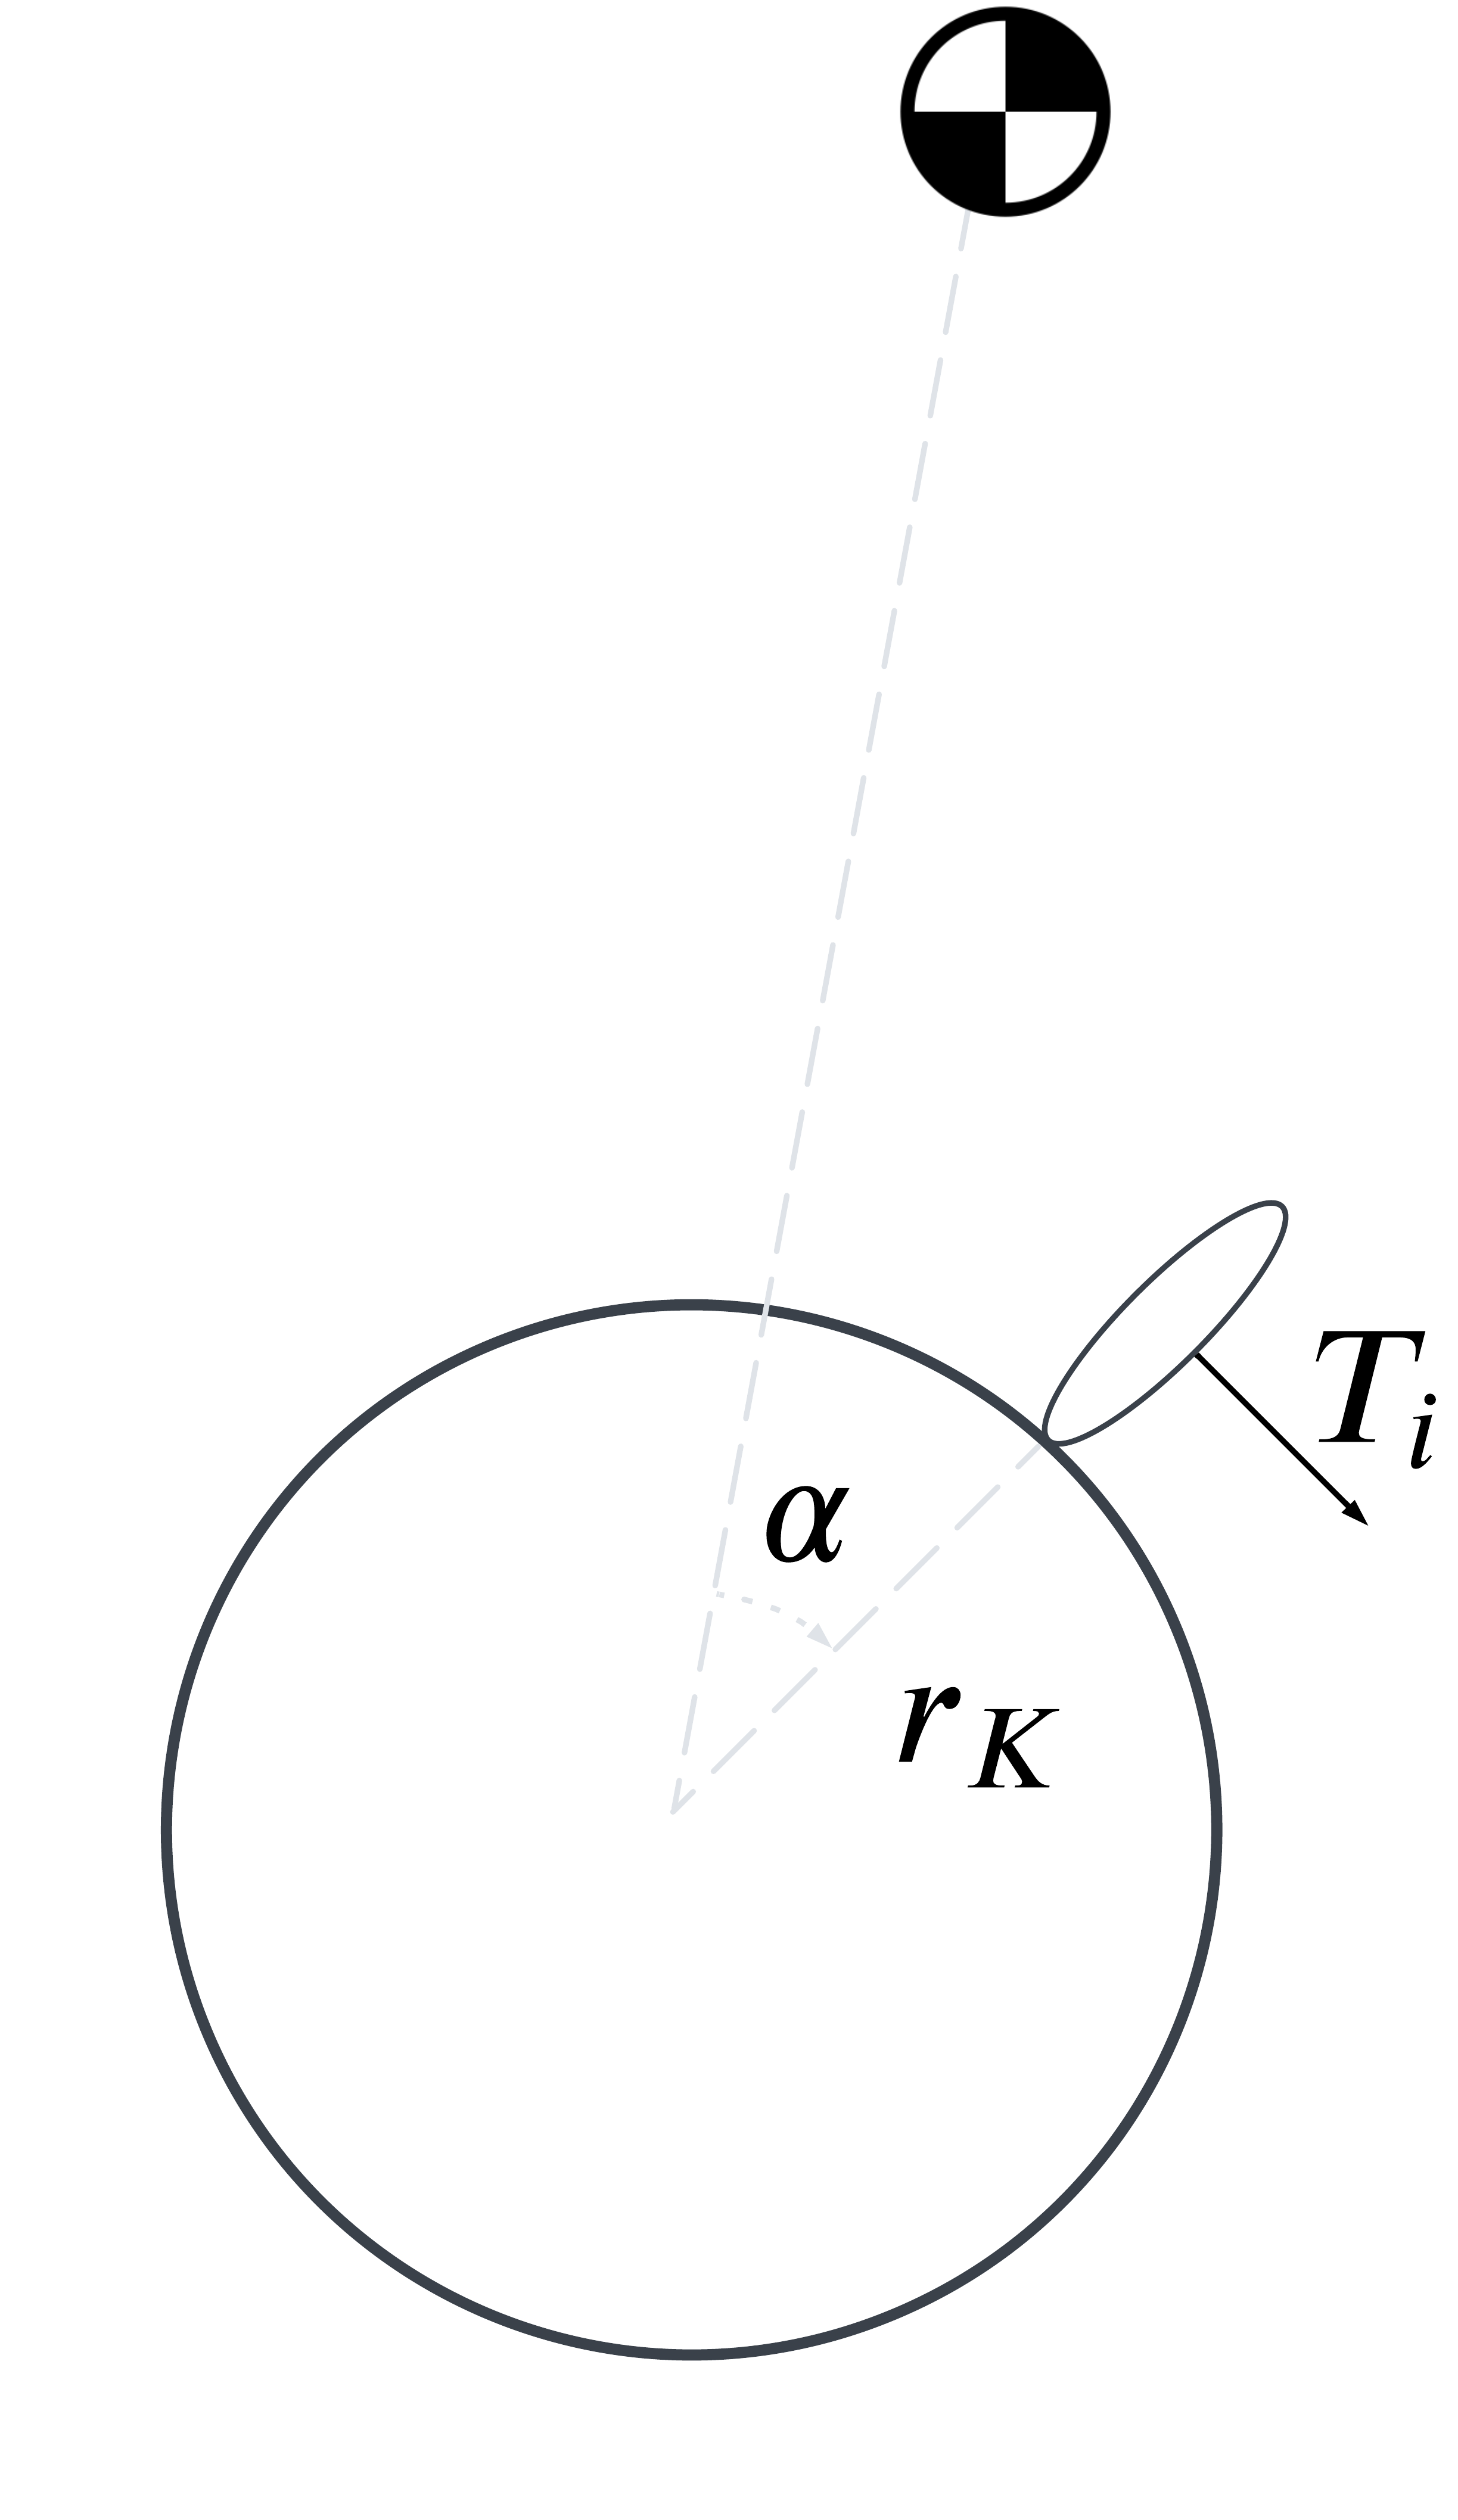
\includegraphics[width=\linewidth]{Metodologia/Figuras/torque_side.png}
        \caption{Modelo real visto de lado}
        \label{fig:torques_lado}
    \end{subfigure}
    \hfill
    \begin{subfigure}[b]{0.4\textwidth}
        \centering
        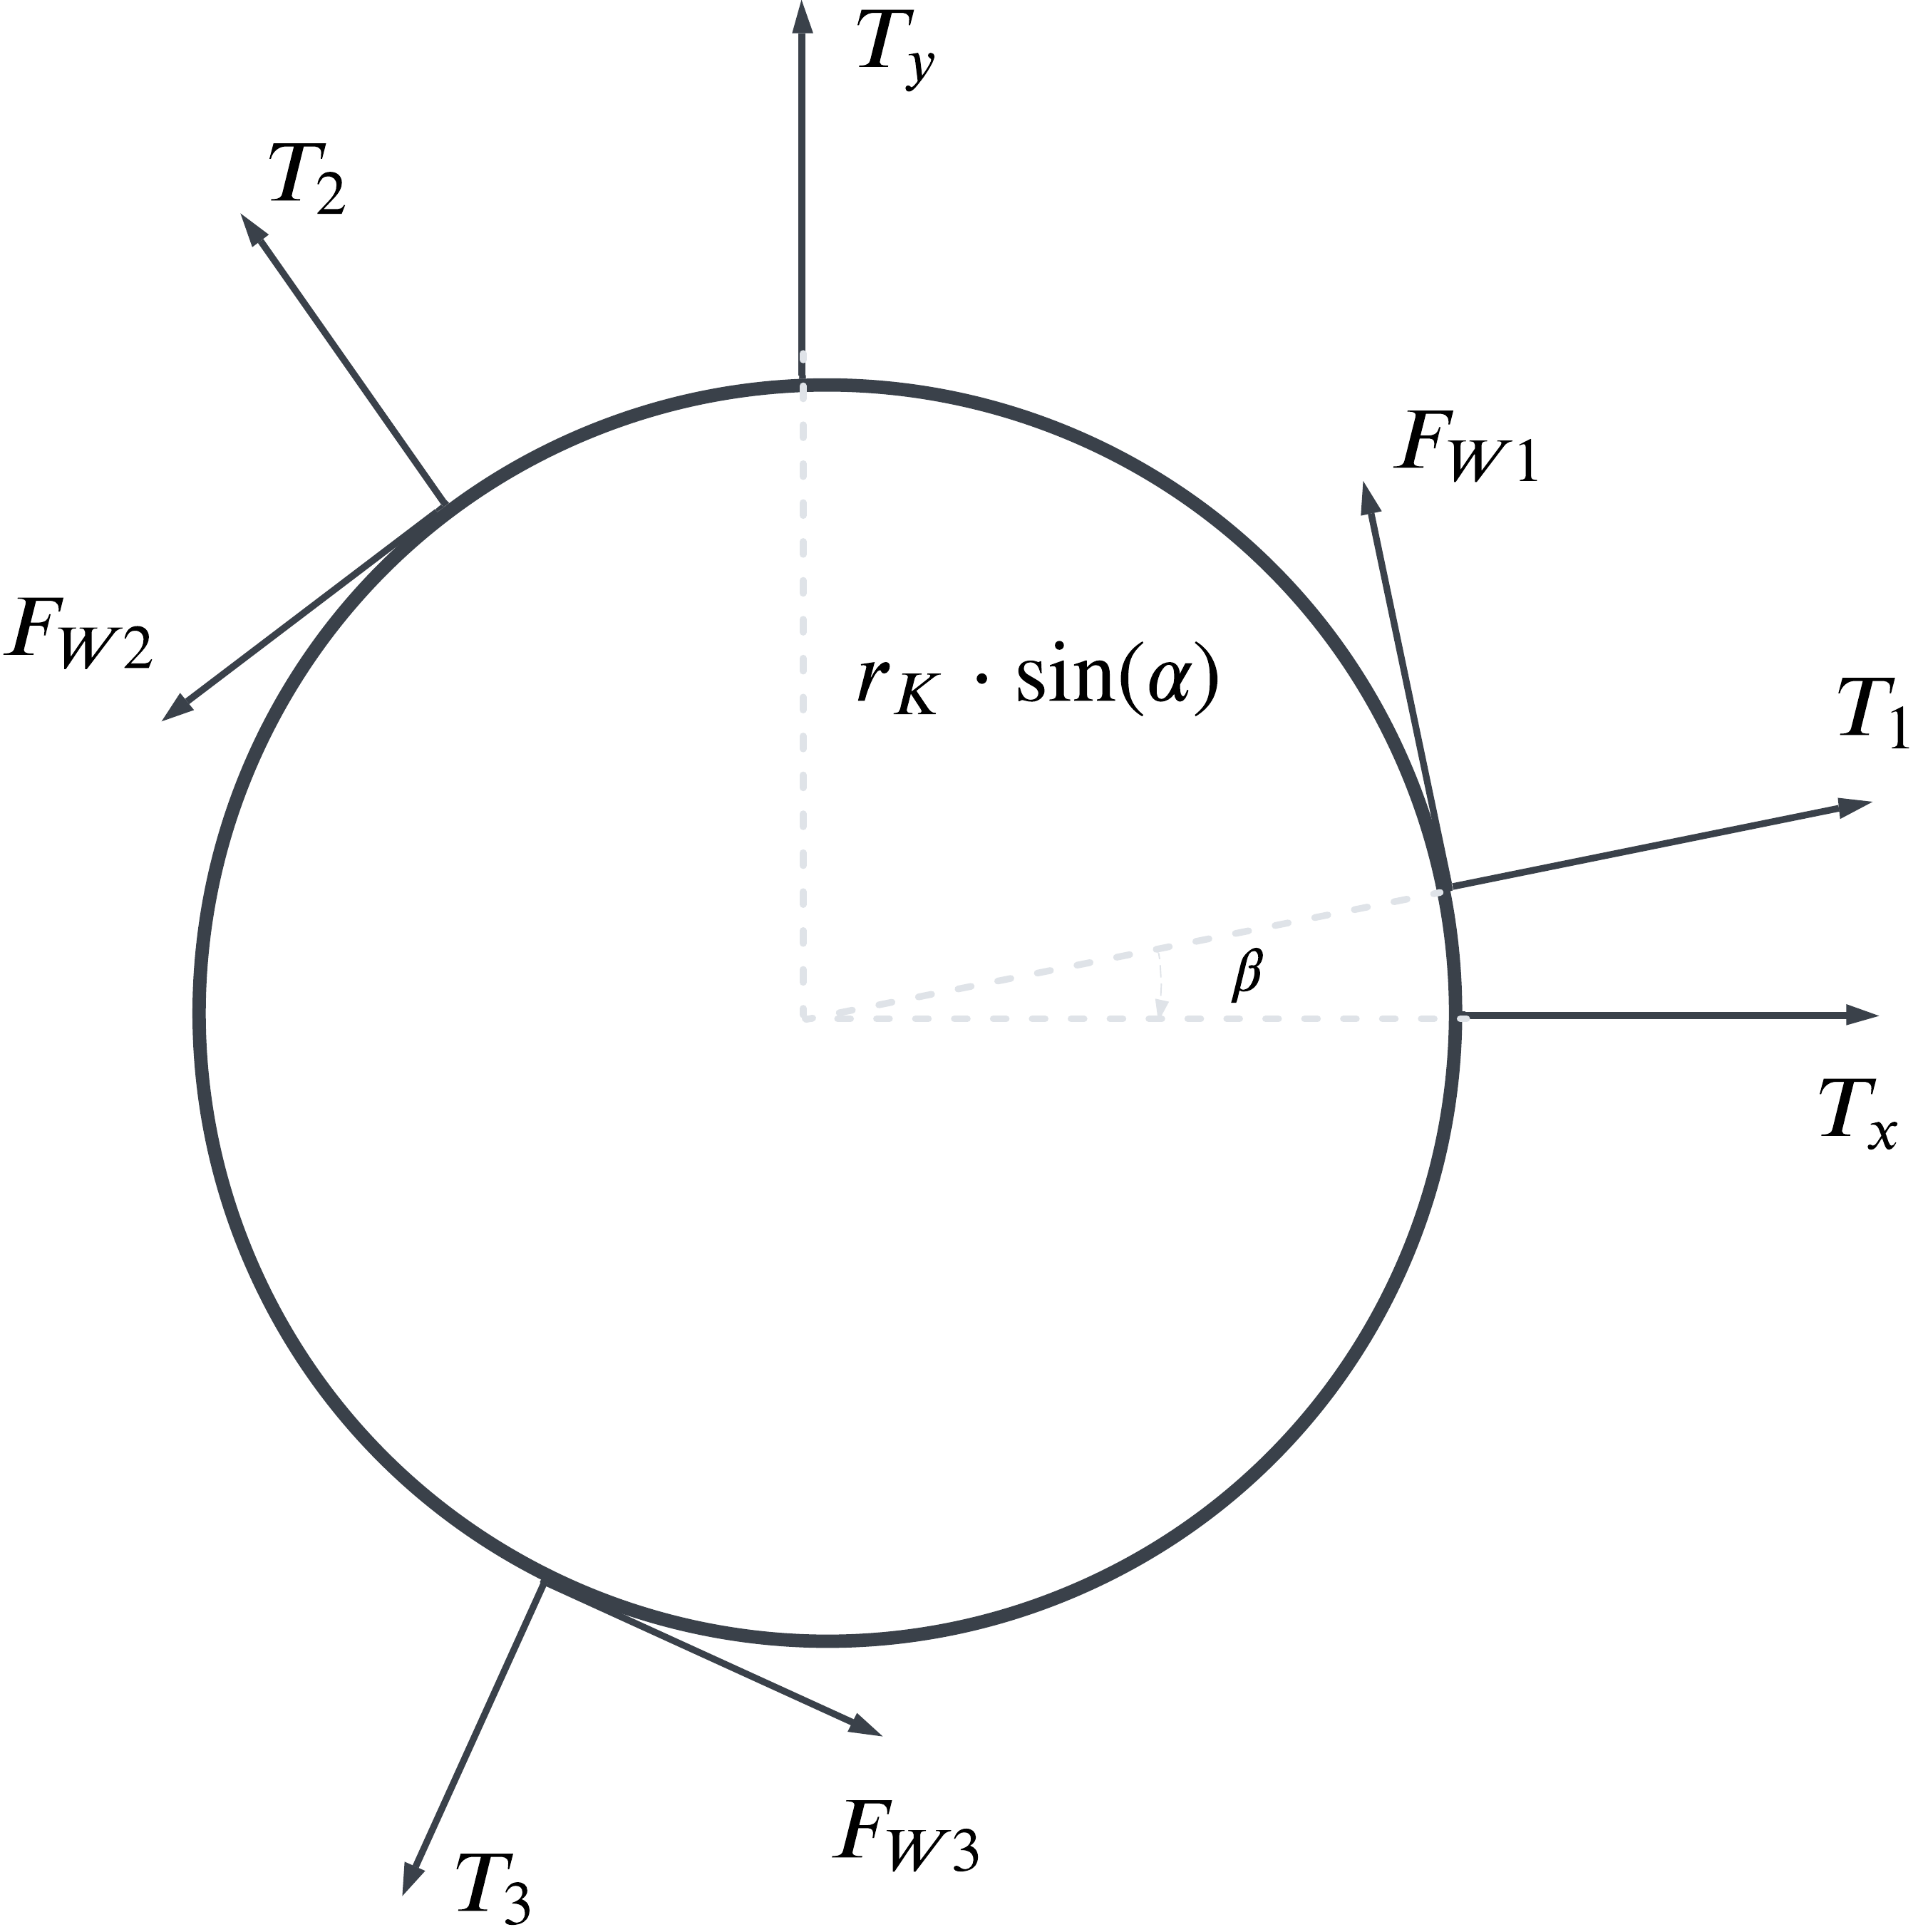
\includegraphics[width=\linewidth]{Metodologia/Figuras/torque_up.png}
        \caption{Modelo real visto de cima}
        \label{fig:torques_cima}
    \end{subfigure}
\end{figure}

Usando esses modelos, obteve-se as forças tangentes provocadas pelo torque dos motores:

\begin{equation}
    \begin{aligned}
    F_{W,1} &= \frac{T_1}{r_W} 
    \begin{bmatrix}
    -\sin \beta \\
    \cos \beta \\
    0
    \end{bmatrix}, \\
    F_{W,2} &= \frac{T_2}{r_W} 
    \begin{bmatrix}
    -\sin \left( \beta + \frac{2}{3}\pi \right) \\
    \cos \left( \beta + \frac{2}{3}\pi \right) \\
    0
    \end{bmatrix}, \\
    F_{W,3} &= \frac{T_3}{r_W} 
    \begin{bmatrix}
    -\sin \left( \beta - \frac{2}{3}\pi \right) \\
    \cos \left( \beta - \frac{2}{3}\pi \right) \\
    0
    \end{bmatrix}.
    \end{aligned}
\end{equation}

Os braços de alavanca também foram obtidos:

\begin{equation}
    \begin{aligned}
        r_{KW,1} &= r_K \cdot 
        \begin{bmatrix}
        \cos \beta \sin \alpha \\
        \sin \beta \sin \alpha \\
        \cos \alpha
        \end{bmatrix}, \\
        r_{KW,2} &= r_K \cdot 
        \begin{bmatrix}
        \cos \left( \beta + \frac{2}{3}\pi \right) \sin \alpha \\
        \sin \left( \beta + \frac{2}{3}\pi \right) \sin \alpha \\
        \cos \alpha
        \end{bmatrix}, \\
        r_{KW,3} &= r_K \cdot 
        \begin{bmatrix}
        \cos \left( \beta - \frac{2}{3}\pi \right) \sin \alpha \\
        \sin \left( \beta - \frac{2}{3}\pi \right) \sin \alpha \\
        \cos \alpha
        \end{bmatrix}.
    \end{aligned}
\end{equation}

Ainda, obteve-se as forças tangentes nos modelos planares e seus braços de alavanca:

\begin{equation}
    \begin{aligned}
    F_{W,x} &= \frac{T_x}{r_W} \cdot 
    \begin{bmatrix}
    0 \\ 
    1 \\ 
    0
    \end{bmatrix}, \\
    F_{W,y} &= \frac{T_y}{r_W} \cdot 
    \begin{bmatrix}
    1 \\ 
    0 \\ 
    0
    \end{bmatrix}, \\
    F_{W,z} &= \frac{T_z}{r_W} \cdot 
    \begin{bmatrix}
    -\sin \beta \\ 
    \cos \beta \\ 
    0
    \end{bmatrix}, \\
    r_{KW,x} = r_{KW,y} &= r_K \cdot 
    \begin{bmatrix}
    0 \\ 
    0 \\ 
    1
    \end{bmatrix}, \\
    r_{KW,z} &= r_K \cdot 
    \begin{bmatrix}
    \cos \beta \cdot \sin \alpha \\ 
    \sin \beta \cdot \sin \alpha \\ 
    0
    \end{bmatrix}.
    \end{aligned}
\end{equation}

Portanto, os torques na bola no modelo real e nos modelos planares são:

\begin{equation}
    \begin{aligned}
    T_{KW,i} &= r_{KW,i} \times F_{W,i} \quad \text{para } i = 1, 2, 3, \\
    T_{KW,j} &= r_{KW,j} \times F_{W,j} \quad \text{para } j = x, y, z.
    \end{aligned}
\end{equation}

Como o torque total deve ser conservado, usou-se a equação

\begin{equation}
    T_{KW,1} + T_{KW,2} + T_{KW,3} = T_{KW,x} + T_{KW,y} + T_{KW,z}
\end{equation}

para calcular o torque dos motores reais e o torque dos motores virtuais:

\begin{align*}
T_1 &= \frac{1}{3} \left( T_z + \frac{2}{\cos \alpha} \cdot \left( T_x \cdot \cos \beta - T_y \cdot \sin \beta \right) \right) \\
T_2 &= \frac{1}{3} \left( T_z + \frac{1}{\cos \alpha} \cdot \left( \sin \beta \cdot \left( -\sqrt{3} T_x + T_y \right) - \cos \beta \cdot \left( T_x + \sqrt{3} T_y \right) \right) \right) \\
T_3 &= \frac{1}{3} \left( T_z + \frac{1}{\cos \alpha} \cdot \left( \sin \beta \cdot \left( \sqrt{3} T_x + T_y \right) + \cos \beta \cdot \left( -T_x + \sqrt{3} T_y \right) \right) \right)
\end{align*}

\begin{align*}
T_x &= \cos \alpha \cdot \left( T_1 \cdot \cos \beta - T_2 \cdot \sin \left( \beta + \frac{\pi}{6} \right) + T_3 \cdot \sin \left( \beta - \frac{\pi}{6} \right) \right) \\
T_y &= \cos \alpha \cdot \left( -T_1 \cdot \sin \beta - T_2 \cdot \cos \left( \beta + \frac{\pi}{6} \right) + T_3 \cdot \cos \left( \beta - \frac{\pi}{6} \right) \right) \\
T_z &= T_1 + T_2 + T_3
\end{align*}

\subsection{Cálculos de inércia}

A inércia da bola foi aproximada por uma esfera oca, 

\begin{equation*}
    \Theta_K = \frac{2}{3} \cdot m_K \cdot r_K^2,
\end{equation*}

enquanto o corpo foi aproximado por um cilindro:

\begin{equation*}
    \Theta_A = \frac{1}{4} \cdot m_A \cdot r_A^2 + \frac{1}{2} \cdot m_A \cdot h^2 + m_A \cdot l^2,
\end{equation*}

\begin{equation*}
    \Theta_{A,xy} = \frac{1}{2} \cdot (m_A + m_W) \cdot r_A^2.
\end{equation*}

Dado o momento de inércia do motor, $\Theta_M$, e o momento de inércia da roda omnidirecional,

\begin{equation}
    \Theta_{OW} = \frac{1}{2} \cdot m_{OW} \cdot r_W^2
\end{equation},

onde $m_{OW}$ é a massa da roda omnidirecional.

Ainda, há o momento de inércia das rodas virtuais, que foi obtido comparando a energia rotacional em torno de um eixo no sistema virtual com a energia rotacional em torno do mesmo eixo no sistema real.

As velocidades angulares da rodas na direção $y$ são:

\begin{align*}
\omega_{OW,1} &= \omega_{W,x} \cos \alpha \\
\omega_{OW,2/3} &= -\frac{1}{2} \omega_{W,x} \cos \alpha
\end{align*}

Enquanto na direção $x$ são:

\begin{align*}
\omega_{OW,1} &= 0 \\
\omega_{OW,2} &= -\frac{\sqrt{3}}{2} \omega_{W,y} \cos \alpha \\
\omega_{OW,3} &= \frac{\sqrt{3}}{2} \omega_{W,y} \cos \alpha
\end{align*}

Por fim, na direção z:

\begin{equation*}
    \omega_{OW,1/2/3} = \omega_{W,z} \sin \alpha
\end{equation*}.

Fazendo o quilibrio energético na direção y,
\begin{align*}
\frac{1}{2} \Theta_{W,x} \dot{\psi}_x^2 &= \frac{1}{2} \Theta_{OW} (\dot{\psi}_x \cos \alpha)^2 + \frac{1}{2} \Theta_M (\dot{\psi}_x \cos \alpha)^2 \\
&\quad + \frac{1}{2} \cdot 2 \left( \Theta_{OW} \left(-\frac{1}{2} \dot{\psi}_x \cos \alpha \right)^2 + \Theta_M \left(-\frac{1}{2} \cdot \dot{\psi}_x \cos \alpha \right)^2 \right) \\
\Theta_{W,x} &= \cos^2(\alpha) \left( \Theta_{OW} + \Theta_M + \frac{1}{2} \left( \Theta_{OW} + \Theta_M \right) \right) \\
&= \frac{3}{2} \cos^2(\alpha) \left( \Theta_{OW} + \Theta_M \right)
\end{align*},

e na direção x,
\begin{align*}
\frac{1}{2} \Theta_{W,y} \dot{\psi}_y^2 &= \frac{1}{2} \cdot 2 \left( \Theta_{OW} \left(\frac{\sqrt{3}}{2} \dot{\psi}_y \cos \alpha \right)^2 + \Theta_M \left(-\frac{\sqrt{3}}{2} \cdot \dot{\psi}_x \cos \alpha \right)^2 \right) \\
\Theta_{W,y} &= \frac{3}{2} \cos^2(\alpha) (\Theta_{OW} + \Theta_M),
\end{align*}

usando a notação.

\begin{align*}
\dot{\psi}_x &= \omega_{W,x} \\
\dot{\psi}_y &= \omega_{W,y} \\
\dot{\psi}_1 &= \omega_{OW,1} \\
\dot{\psi}_2 &= \omega_{OW,2} \\
\dot{\psi}_3 &= \omega_{OW,3}.
\end{align*}

tem-se, portanto,

\begin{align*}
\Theta_{W} = \Theta_{W,x} = \Theta_{W,y} = \frac{3}{2} \cos^2(\alpha) (\Theta_{OW} + \Theta_M).
\end{align*}

Seguindo-se o mesmo procedimento para o plano $x$-$y$ obteve-se:

\begin{align*}
    \Theta_{W,xy} = 3 \cdot (\Theta_{OW} + i^2 \cdot \Theta_M).
\end{align*}


\section{Projeto de controladores}
\label{sec:projetocontroladores}

\clearpage
\chapter{Resultados}

Para a execução do projeto, algumas etapas de desenvolvimento tiveram de ser seguidas: familiarização com o sistema, estudo dos módulos envolvidos, leitura dos requisitos, elaboração de documento descrevendo todo o processo de implementação e relacionamento com os diversos módulos, implementação e testes.


\section{Atividades do Projeto}
\label{metodo3}

\section {Requisitos do Sistema}
\label{req}


\section{Desenvolvimeto e Implementação}

A Tabela \ref{tab:tabela} apresenta as atividades executadas.

\begin{table}
\centering
%Note os alinhamentos diferentes em cada coluna
\begin{tabular}{|c|r|l|}\hline
		Atividade 1 & aa  & ab  \\ 
					 & a & b \\ \hline
		Ativ. 2  & aa & ab \\			
					 &  a & b \\ \hline
		\end{tabular}
	\caption{Exemplo de tabela - Coloque toda informação sobre a tabela aqui}
	\label{tab:tabela}
\end{table}

\section{Testes}

\section{Análise dos Resultados}

Apresente os resultados sem adulterações e faça análises objetivas. Pense na melhor maneira de apresentar os resultados graficamente. Se os gráficos são difíceis de interpretar, talvez tabelas sejam uma forma melhor de apresentar resultados. Não apresente dados (gráficos e tabelas) se não há uma conclusão interessante a ser tirada. Lembre-se de ser conciso.

\emph{Não se esqueça das unidades!} Pense que \emph{a priori} todo número deve ter uma unidade. Não escreva as unidades em itálico (no ambiente matemático) e tome cuidado para diferenciar maiúsculas e minúsculas. Um exemplo é escrever $22$ [kN] e não $22 KN$ (Kelvin vezes Newton!).

Ao apresentar resultados experimentais, tome o cuidado para também apresentar o cálculo das incertezas sempre que forem significativas. Ao fazer conclusões, sempre considere se o tamanho da sua amostra é grande o suficiente do ponto de vista estatístico. Lembre que a média empírica $\hat{\mu}_X$ de $N$ observações independentes da variável $X_i$ possui variância
\[
\hat{\sigma}_{\mu}^2 = \frac{1}{N(N-1)} \sum_{i=1}^N (X_i-\hat{\mu}_X)^2
\enspace,
\]
onde se assume que as variáveis $X_i$ possuem uma mesma ditribuição e que essa distribuição possui segundo momento finito.


\section{Resumo do Capítulo}
\label{sec:resumoo4}
Tente não terminar de forma abrupta. Se for escrever algo aqui, não seja genérico!

\section{Formato, expressões matemáticas e o \LaTeX}

\subsection{O \LaTeX}

O {\LaTeX}  é o método preferencial de preparação de documentos para textos técnicos nas ciências exatas. O {\LaTeX} permite não só lidar com equações de uma forma mais prática que em editores de texto, mas também facilita a formatação de documentos e tem um desempenho marcadamente superior a editores de texto na preparação de documentos longos como monografias. 

Documentos em {\LaTeX} são escritos em um ou mais arquivos de texto com extensão .tex. Após a escrita, o .tex é \emph{compilado} para gerar arquivos nos formatos .pdf, .dvi ou .ps. Hoje há duas distribuições padrão para o \LaTeX. Sistemas Windows usam o {Mik\TeX} e sistemas Unix usam o \TeX Live. Além das distribuições, muitos usuários utilizam \emph{front-ends} que facilitam a edição do texto, a compilação e a instalação de pacotes. 

Os pacotes necessários para compilar o presente documento devem ser encontrados numa instalação completa dessas distribuições. Se tiver dificuldades com os pacotes, você pode instalá-los manualmente ou tentar alterar o código para usar versões antigas dos mesmos.

A compilação pode ser feita pelos comandos \textsf{latex} ou \textsf{pdflatex}, invocados pela linha de comando ou pelo \emph{front-end}. Note que será necessário empregar o comando \textbf{mais de uma vez} para que as referências cruzadas saiam corretas.

Como discutido na Seção \ref{sec:revisão}, uma ferramenta útil para gerenciar as citações em {\LaTeX} é o Bib\TeX. Para gerar uma lista bibliográfica a partir do arquivo .bib, este arquivo deve ser indicado no arquivo .tex. Em seguida devem-se executar os comandos \textsf{pdflatex}, \textsf{bibtex} e \textsf{pdflatex} novamente sempre usando o .tex como argumento. Note que os comandos são executados nesta ordem e de forma repetida para que as referências cruzadas sejam geradas corretamente.

Nesta seção você deve encontrar exemplos dos comandos mais usados em \LaTeX. Outros exemplos e manuais podem ser encontrados na internet com facilidade.

\subsection{Expressões Matemáticas}

Ao escrever expressões matemáticas, defina todas as variáveis antes de usá-las ou imediatamente depois da expressão. Deixar de fazê-lo torna seu texto \textbf{ilegível}. Segue um exemplo.

Seja o par $(a_1,a_2)\in \mathbb{R}^2$. Para $s\in\mathbb{C}$, definimos a função $f(s)$ como
\[%cria equações sem numeração
f(s)\triangleq \frac{a_1 s+a_2}{s^2+2\zeta\omega_n s+\omega_n^2}
\enspace,
\]
onde os escalares $\zeta,\omega_n>0$ são constantes.

Note que não foi necessário atribuir valores às variáveis neste momento. Repare também como devemos \textbf{usar pontuação} (vírgula) nas equações, tratando-as como parte da frase. Usamos o símbolo $\triangleq$ ou $:=$ para deixar explícito que se trata de uma definição. Ser claro nesse aspecto facilita o entendimento do leitor.

A equação acima não foi numerada porque não será citada no texto. Vejamos um exemplo com numeração.

A função $f(\cdot)$ possui um zero em $-a_2/a_1$ (ou $-\frac{a_2}{a_1}$) e, para $\zeta<1$, possui polos complexos $p_{1,2}$ dados por
\begin{equation}
\label{eq:polos}
p_{1,2}=\omega_n \left(-\zeta\pm j\sqrt{1-\zeta^2}\right)
\enspace.
\end{equation}
Agora podemos citar os polos dados pela Equação (\ref{eq:polos}) (aqui adotamos a convenção de citar sempre com o número entre parênteses precedido da palavra Equação). Note como usamos um comando especial na Equação \ref{eq:polos} para garantir o ajuste automático do tamanho dos parênteses.

Vejamos agora como criar equações alinhadas. Considere o sistema dinâmico dado pelas equações diferenciais:

\begin{align}
\dot{x}_1 & = \cos(x_2)\cdot\ln(1/x_1)+\tan(u) \label{eq:x1dot} \\
\dot{x}_2 & = e^{-x_1-x_2} \nonumber \\
& y  = \min\{x_1,x_2\}  \label{eq:saida}
\enspace,
\end{align}
onde $x(t)=[x_1(t) ~ x_2(t)]'$, $t>0$, é a variável de estado do sistema, $u(t)$ é o sinal de entrada e $y(t)$ é o sinal de saída do sistema. Note no .tex que o caracter de tabulação \textsf{\&} foi usado para indicar o ponto de alinhamento horizontal das equações. Além disso, para ilustrar o uso do \LaTeX, retiramos a numeração da segunda equação e citamos as equações separadamente.

Nas Equações (\ref{eq:x1dot}) e (\ref{eq:saida}), aparecem operadores como $\min$, $\ln$, $\cos$ e $\tan$. A convenção aqui é que \textbf{variáveis devem ser escritas em itálico e operadores não}. Por essa razão todas as expressões matemáticas devem ser escritas no ambiente matemático (entre cifrão) mesmo quando for possível usar texto comum. Isso garante a consistência das fontes utilizadas (nem sempre a fonte do ambiente matemático é a mesma fonte do texto). 

Para escrever matrizes, podemos fazer por exemplo:
\[
\sum_{n=0}^{\infty}z^{-n}\left[\begin{array}{cc}
\lambda & 1 \\
0 & \lambda
\end{array}\right]^n=
\left[\begin{array}{cc}
\frac{z}{z-\lambda} & \frac{z}{(z-\lambda)^2} \\
0 & \frac{z}{z-\lambda}
\end{array}\right]
,~\forall \lambda<|z|
\enspace.
\]

Para escrever uma expressão com múltiplos casos, podemos fazer, para um inteiro $N$ positivo,
\[
g[n]=
\left\{
\begin{array}{ll}
0,& \mbox{se }~ n\leq 0 \\
n,& \mbox{se }~ n=1,2,\ldots,N-1 \\
N,& \mbox{se }~ n\mod N = 0 \\
0,& \mbox{caso contrário}\enspace.
\end{array}
\right.
\]

\textbf{Nunca reaproveite símbolos} matemáticos, isto é, nunca use o mesmo símbolo para designar variáveis diferentes.

Para um exemplo com múltiplas linhas de expressão matemática: tem-se que, para $a\neq 0$,

\begin{equation}
\begin{split}
ax^2+bx+c &= 0 \\
& \Rightarrow a(x^2+bx/a+c/a) =0 \Rightarrow a((x+b/(2a))^2+c/a-b^2/(4a^2))=0  \\
& \Rightarrow (x+b/(2a))^2=(b^2-4ac)/(4a^2) \\
& \Rightarrow (x+b/(2a))=\pm\sqrt{b^2-4ac}/(2a) \\
& \Rightarrow x=\frac{-b\pm\sqrt{b^2-4ac}}{2a}
\enspace.
\end{split}
\end{equation}

Note a argumentação lógica aqui. Não estamos dizendo que o valor de $x$ é dado pela última linha. Estamos dizendo que a hipótese da primeira linha juntamente com a hipótese $a\neq 0$ implicam os referidos valores de $x$. \textbf{Um erro comum dos alunos ao escrever é não distinguir a veracidade das implicações com a veracidade das hipóteses}.

\clearpage
\chapter{Conclusões}

Novamente, este será um dos trechos que o leitor experiente lerá antes de decidir se vale a pena ler o texto integral. Seja convincente.

\section{Considerações Finais}

Reitere o que de mais importante foi feito, qual era o objetivo inicial e qual o resultado obtido. Se houve requisitos ou especificações de projeto, discuta se foram atingidos. Se os resultados não foram conclusivos ou contrariam o que se esperava, seja honesto e diga-o explicitamente. Busque explicar os insucessos com argumentos sólidos e plausíveis. 

\section{Propostas de Continuidade}

Se houve questões ainda não respondidas ou resultados insatisfatórios, aponte direções de continuação.

\clearpage


\addcontentsline{toc}{chapter}{Referências Bibliográficas}
\renewcommand{\bibname}{Referências Bibliográficas}

%\bibliographystyle{abntex2-alf} %para norma ABNT no sistema autor-data
\bibliographystyle{abntex2-num}
\begin{small}
\bibliography{ListadeReferencias}%,library}
%% Monografia para Projeto de Fim de Curso - Exemplo no LaTeX
%-----------------------------------------------------------


%---------------Inicialização de pacotes--------------------

\documentclass[12pt,a4paper,notitlepage,twoside]{book}


\usepackage{graphicx}
\usepackage[utf8]{inputenc}
%\usepackage[latin1]{inputenc} %%pode ser necessário trocar a codificação em sistemas Windows
\usepackage[brazil]{babel}		%%pode ser necessário trocar o pacote de línguas em algumas distribuições LateX
%\usepackage[portuguese]{babel}
\usepackage[T1]{fontenc}
\usepackage{amsmath,amssymb}
\usepackage{amsthm,amsfonts}
\usepackage{color}
\usepackage[colorlinks]{hyperref}
\usepackage{abntex2abrev}
%\usepackage[alf]{abntex2cite} %se você quiser seguir as normas ABNT no sistema autor-data
%\usepackage[num]{abntex2cite} %se você quiser seguir as normas ABNT no sistema numérico
\usepackage{setspace}
\usepackage[toc,page]{appendix}

%Definindo fonte Times (Use os pacotes obsoletos se não conseguir instalar os atualizados)
%\usepackage{times}     %Pacote de fontes obsoleto, apenas texto
%usepackage{mathptmx}  %Pacote de fontes obsoleto, texto e símbolos matemáticos
%\usepackage{newtxtext,newtxmath}  %Pacotes de fontes mais recentes

\usepackage[a4paper,top=30mm,bottom=30mm,inner=30mm,outer=25mm,headheight=7mm,headsep=6mm,footskip=7mm]{geometry}
\usepackage{enumerate}
\usepackage{tabularx}
\usepackage{array} % Necessário para o alinhamento vertical
\usepackage{makecell} % Para controle uniforme da altura das linhas
\usepackage{float}    % Para fixar a tabela no local desejado
\usepackage{subcaption} % Alinhar imagens lado a lado
\usepackage{graphicx} % Reduzir tamanho da fonte de uma equação

\makeindex

%\singlespacing   %%espaçamento simples
%\onehalfspacing
%\setstretch{1.03} %%um pouco melhor que espaçamento simples
\linespread{1.25} %corresponde ao espaçamento 1.5 do MS Word

%---------------Início do documento-------------------------

\begin{document}

\setlength{\extrarowheight}{4pt} % Define uma altura extra para as linhas

\begin{titlepage}
\begin{center}
{\large Universidade Federal de Minas Gerais\\
Escola de Engenharia \\
Curso de Graduação em Engenharia de Controle e Automação\\}

\vspace{6cm}
{\bf\Large Construção, modelagem, projeto de controlador e implementação em hardware para um pêndulo invertido sobre uma esfera\vspace{0.2cm}}
\vspace{4cm}

%\hspace{0.3\textwidth} \parbox{0.65\textwidth}
{\large Samuel Soares do Patrocínio}
\vspace{2cm}  
   
\vspace{2cm}          
%\hspace{0.3\textwidth} 
{\large Orientador: Prof. Fernando de Oliveira Souza}\\
%{\large Supervisor: Eng. Cicrano}

\vfill
%\hspace{0.3\textwidth} 
{\large Belo Horizonte, Novembro de 2024 }
\end{center}

\end{titlepage}

\newpage
\clearpage
\thispagestyle{empty}


\begin{titlepage}

\centering
\textbf{Monografia}\\
\vspace{2cm}
\centering
\textbf{Construção, modelagem, projeto de controlador e implementação em hardware para um pêndulo invertido sobre uma esfera}\\
\vspace{5cm} 

\parbox{1.0\textwidth} 
{\large 
Monografia submetida à banca examinadora
designada pelo Colegiado Didático do Curso de
Graduação em Engenharia de Controle e
Automação da Universidade Federal de Minas
Gerais, como parte dos requisitos para aprovação na
atividade Projeto Final de Curso II.}

\vspace{7cm} 
\centering
Belo Horizonte, Julho de 2014

\end{titlepage}


\pagenumbering{roman}
\addcontentsline{toc}{chapter}{Resumo}

\begin{center}
\huge{{\bf Resumo}}
\vspace{2cm}
\end{center}

No Resumo, em uma única página, em no máximo dois parágrafos, você explicita os seguintes itens: objetivos do projeto e descrição sucinta do local onde ele foi desenvolvido; metodologia utilizada; e resultados alcançados. Leitores experientes decidem se prosseguirão para a leitura do texto completo após lerem o resumo, a conclusão e a introdução. Por isso nestes lugares você deve colocar um esforço maior de convencimento. Além disso, a linguagem utilizada deve ser acessível a leitores com pouca familiaridade com a área, limitando-se o uso de jargões.
 
\begin{sloppypar}
Este novo parágrafo serve para mostrar que ao pular uma ou mais linhas no texto do arquivo .tex, o \TeX\ entende que você está iniciando outro parágrafo. O comando \textsf{sloppypar} força o texto a não ultrapassar as margens. Só deve ser usado se este problema ocorrer.
\end{sloppypar}

 
\clearpage
\thispagestyle{empty}
\cleardoublepage


\addcontentsline{toc}{chapter}{Abstract}

\begin{center}
\huge{{\bf Abstract}}
\vspace{2cm}
\end{center}

Write a version of your ``resumo'' in English. Beware of literal translations and double check the translation of technical terms.
 

 
\clearpage
\thispagestyle{empty}
\cleardoublepage


\addcontentsline{toc}{chapter}{Agradecimentos}

\begin{center}
\huge{{\bf Agradecimentos}}
\vspace{4cm}
\end{center}

Aqui vai o texto dos agradecimentos.
 
\clearpage
\thispagestyle{empty}
\cleardoublepage
\tableofcontents
%\markboth{Conteúdo}{Conteúdo}

\clearpage
%\thispagestyle{empty}
%\cleardoublepage

% Normalmente, este arquivo só contém isto.
\listoffigures
\addcontentsline{toc}{chapter}{Lista de Figuras}
%\markboth{Lista de Figuras}{Lista de Figuras}

\clearpage
%\thispagestyle{empty}
%\cleardoublepage

% Normalmente, este arquivo só contém isto.
\listoftables
\addcontentsline{toc}{chapter}{Lista de Tabelas}
%\markboth{Lista de Tabelas}{Lista de Tabelas}

\clearpage
%\thispagestyle{empty}
%\cleardoublepage

% Normalmente, este arquivo só contém isto.

\pagenumbering{arabic}
\setcounter{page}{1}
\chapter{Introdução}
\label{chap:intro} %este label será usado para referenciar este capítulo

%As primeiras frases têm a missão de prender a atenção do leitor e por isso são as mais importantes do texto. Diga o quanto antes o que você fez e quais são os resultados alcançados. Ao terminar de ler a introdução o leitor tomará uma nova decisão de se vale a pena ou não continuar lendo o texto. Capte a atenção do leitor bem aqui.

%A comunicação escrita é considerada umas das cinco habilidades mais importantes por profissionais de engenharia e um engenheiro passa em média mais de $25$\% do seu tempo escrevendo \cite{eggert2002response,spretnak1982survey}. Uma quantidade similar de tempo é gasta na escrita de correspondência e de relatórios técnicos \cite{cunningham2012perceptions}. Dessa forma, encare a escrita do seu projeto como um treinamento nessa importante habilidade.

%Neste texto você encontrará não apenas uma estrutura para escrever seu trabalho em \LaTeX, mas também um pequeno manual de boas práticas na escrita técnica. Leia com atenção e coloque as sugestões em prática à medida que preenche o texto com o conteúdo do seu próprio projeto. Também será apresentado um número de vícios de escrita comumente encontrados nas monografias de alunos. 

%A seguir está a estrutura de organização sugerida pelo colegiado do curso. Note que ela não é necessariamente a melhor para contar a história do seu projeto. Você pode por exemplo preferir usar títulos mais pertinentes ao seu contexto. Contudo, o seu texto deve conter cada um dos pontos a seguir.

\section{Motivação e Justificativa}
\label{sec:motivacao}

O avanço contínuo na área de controle e automação exige que os futuros engenheiros dominem técnicas práticas e teóricas para solucionar problemas reais de engenharia. No contexto do curso de Engenharia de Controle e Automação, é essencial que os alunos tenham acesso a plataformas de aprendizagem que unam teoria e prática de maneira dinâmica e interativa. Nesse cenário, o desenvolvimento de sistemas experimentais versáteis e acessíveis é uma abordagem eficiente para consolidar o aprendizado e despertar o interesse por sistemas de controle complexos.

O projeto proposto consiste na construção de um robô que se equilibra sobre uma esfera, uma aplicação concreta do conceito de pêndulo invertido. Esse sistema é amplamente utilizado no ensino de técnicas de controle devido à sua natureza desafiadora e suas características dinâmicas, que exigem uma compreensão aprofundada de modelagem, análise e implementação de controladores.

A utilização de modelagem 3D e impressão em impressoras 3D para a construção do robô garante um custo reduzido, acessível tanto para o laboratório quanto para alunos interessados em replicar o projeto. Essa abordagem também assegura que eventuais danos à planta possam ser facilmente reparados, incentivando o uso contínuo e livre do sistema pelos discentes. Dessa forma, o projeto atende a dois objetivos principais: a oferta de um sistema dinâmico e interessante para o estudo de controle e a promoção de um ambiente de aprendizagem prático e sustentável.

%Argumente sobre a importância do projeto desenvolvido usando uma visão de alto nível, sem entrar em detalhes. Contextualize seu projeto dentro do local de execução ou da literatura e explique como ele é necessário ou inovador. É possível fazer uma breve revisão bibliográfica, confrontando seu trabalho com outras referências bibliográficas para mostrar a sua contribuição. No quesito contribuição, é muito importante deixar claro o tempo todo que partes do projetos foram executadas por outros e que partes foram executadas por você. Caso contrário, corre-se o risco de inadvertidademente tomar crédito pelo trabalho de outrem, o que pode ter implicações legais. 

\section{Objetivos do Projeto}
\label{sec:objetivos}

Tendo em vista o exposto acima, este projeto tem por objetivos:

\begin{enumerate}[a)]
\item  Projetar e construir um robô do tipo pêndulo invertido que se equilibra sobre uma esfera, utilizando conceitos aprendidos ao longo do curso de Engenharia de Controle e Automação;
\item Tornar a construção viável e replicável por meio da utilização de impressão 3D, proporcionando durabilidade e acessibilidade; 
\item Implementar e validar técnicas de controle avançadas para garantir a estabilidade do sistema e seu funcionamento eficiente.

Esses objetivos foram estabelecidos com a finalidade de integrar o conhecimento teórico adquirido ao longo do curso com aplicações práticas relevantes, contribuindo para a formação de engenheiros mais preparados para lidar com desafios reais.
\end{enumerate}

%O conteúdo desta seção pode se sobrepor um pouco com o da seção anterior, podendo ela ser um sumário dos pontos expostos anteriormente. A escolha do título da seção talvez seja mais apropriada para a fase de proposta do projeto. Afinal, nesta fase se conhecem os objetivos e não os resultados. Por outro lado, fará pouco sentido discutir objetivos quando o projeto está finalizado, especialmente se tais objetivos não foram alcançados. 


\section{Local de Realização}
\label{sec:empresa}

O desenvolvimento do projeto será realizado no Laboratório de Controle da Escola de Engenharia da Universidade Federal de Minas Gerais (UFMG). A impressão das peças será viabilizada por meio de uma impressora 3D disponibilizada pelo professor Fernando de Oliveira Souza, que também supervisionará as etapas práticas e fornecerá o suporte técnico necessário.


\section{Estrutura da Monografia}
\label{sec:organizacao}

Esta monografia está organizada em quatro capítulos, além desta introdução. O Capítulo 1 apresenta uma visão geral do projeto, incluindo sua motivação, objetivos e local de execução. O Capítulo 2 explora os princípios fundamentais relacionados ao pêndulo invertido, detalhando conceitos essenciais para o entendimento do sistema e do controle aplicado. O Capítulo 3 descreve a metodologia adotada no projeto, abrangendo as etapas de modelagem 3D, construção da planta física, modelagem matemática e projeto dos controladores. Por fim, o Capítulo 4 apresenta as conclusões obtidas, as contribuições do projeto e sugestões para trabalhos futuros, além de relatar os principais desafios enfrentados.


\clearpage
\chapter[Descrição do Processo]{Descrição do Problema/Processo ou O Processo de Fazer Alguma Coisa}
\label{chap:descricaoproblema}
%Note que, como nome do capítulo é muito longo, fornecemos um nome abreviado uso no cabeçalho

Se desejar, uma visão geral do capítulo pode ser colocada antes da primeira seção. Este é o capítulo de descrição do processo e formulação do problema. Tendo em vista que se trata de uma monografia de engenharia de controle e automação, em muitos casos será fundamental a apresentação dos sensores e atuadores do processo.


\section{Processo de Fazer Alguma Coisa}
\label{sec:hist}

Cada seção inicia pela descrição do seu conteúdo e pode terminar com um parágrafo de conexão com a seção seguinte. 

Antes de formular o problema, \textbf{não se esqueça de fazer todas as definições necessárias}. Também devem-se detalhar os aspectos complementares da abordagem: se estamos estudando um aspeto particular do problema, se a resposta encontrada é universal ou dependente de simplificações e hipóteses prévias.


\section{Instrumentação do Processo}
\label{sec:instrumentação}

Descreva a aparelhagem e o equipamento utilizados bem como a ligação entre os diversos componentes. Nesta seção e, ao longo de todo o texto, você deve dar detalhes suficientes para que qualquer pessoa consiga reproduzir seus experimentos.

Contudo, \textbf{não disperse o leitor com detalhes irrelevantes} ou aspectos
demasiado técnicos ou formais. Reserve tais detalhes para um
apêndice.

Como uma imagem vale mais que mil palavras, e como usar mil palavras prejudicaria a clareza do texto, ilustramos o processo com a Figura \ref{fig:processo}. Lembrar que toda figura deve ser comentada no texto, você nunca deve colocar figuras que fiquem ``soltas'' no texto.  

\begin{figure}[thpb]
  \centering
  \resizebox{120mm}{!}{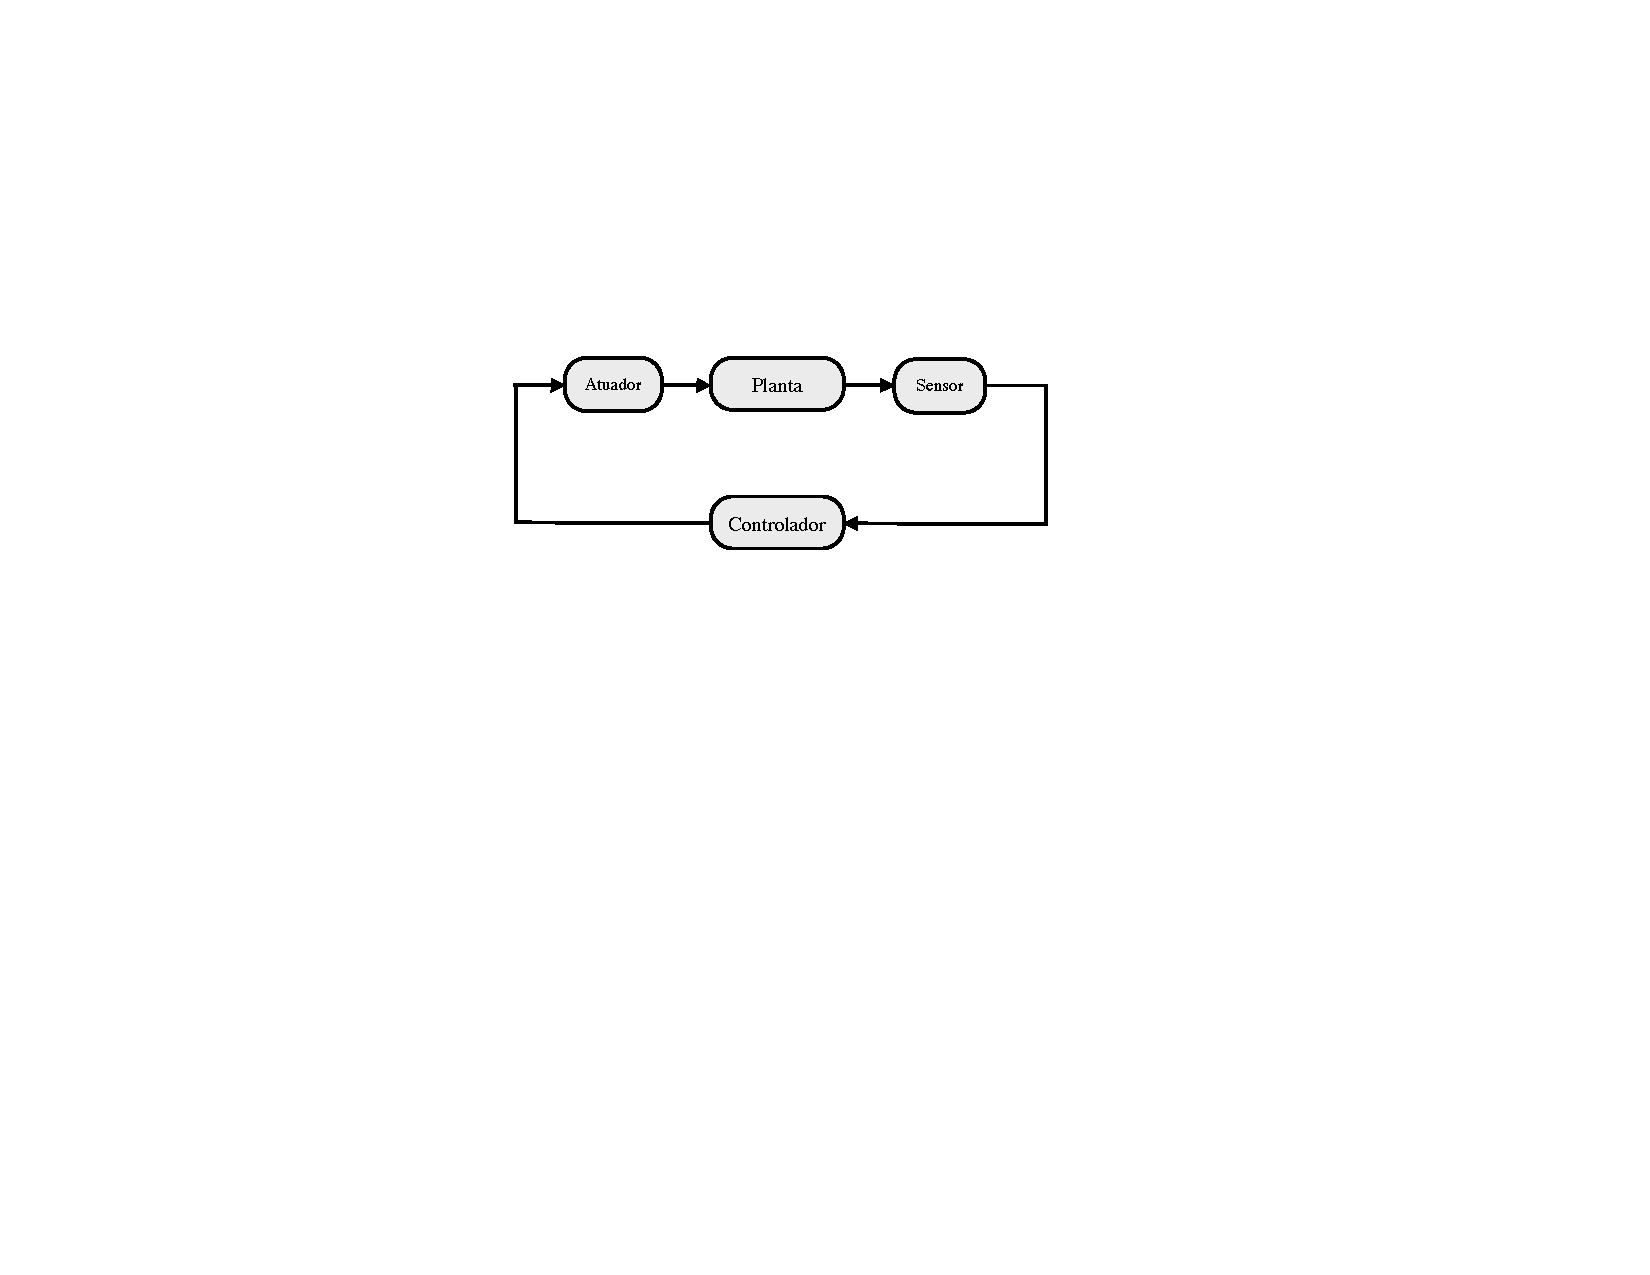
\includegraphics{DescricaoProcesso/Figuras/FiguraProcesso.pdf}}
  \caption{Aqui escrevemos \textbf{toda} informação pertinente à figura. Ou seja, este texto deve ser uma descrição auto-contida da figura, não sendo necessário recorrer ao corpo de texto para saber detalhes sobre a mesma. \emph{Fonte:} Citar fonte se figura 	não for elaborada pelo autor e \textbf{pedir permissão para usar!}}
  \label{fig:processo}
\end{figure}


\section{Situação Atual/Estado da Arte/Revisão da Literatura}
\label{sec:revisão}

Este é o espaço para uma revisão detalhada do enquadramento do problema. Isso inclui descrever a situação atual do processo, aquilo que foi feito até então dentro da empresa/laboratório, e aquilo que se pode chamar de ``Estado da Arte'', ou seja, uma apresentação do conhecimento preexistente
sobre o tema do projeto.

A elaboração desta seção tipicamente demanda uma boa revisão da literatura. Deve haver, quando aplicável uma análise das soluções potencialmente concorrentes, elencando vantagens e desvantagens.

\subsection{Como Elaborar uma Revisão da Literatura}

Ao selecionar referências, devem-se preferir referências de veículos confiáveis, que tenham por exemplo processo de revisão por pares. Portanto, dá-se preferência a artigos em periódicos e livros, em seguida teses e dissertações, artigos em anais de congresso e por fim relatórios. Evitar citar páginas da internet por oferecem menor garantia da informação nelas contida. 

Pesquise sua bibliografia em bases confiáveis como o \textsf{Web of Science}, \textsf{Scopus}, ou o \textsf{Google Scholar}. \textbf{Não use uma ferramenta de busca comum!} (elas não foram feitas pensando no \emph{ranking} de textos científicos) Use o número de citações de uma dada referência como um indicador de sua qualidade. Explore os artigos que citam a referência estudada bem como os artigos que ela cita.

Prefira as referências mais recentes quando se tratar de um assunto na fronteira do conhecimento ou de tecnologia de ponta. Quando se tratar de um assunto já consolidado, prefira citar livros ou artigos com muitas citações. 

Evite citar informações de segunda-mão e procure na medida do possível rastrear a fonte original. Contudo, em situações em que a fonte original é de acesso mais difícil, seja por ter tido publicação limitada como no caso de relatórios ou por não ser em língua inglesa ou portuguesa, é preferível a citação de segunda-mão em um veículo mais acessível.

Para gerenciar suas referências, use uma ferramenta de software como o \textsf{Mendeley}, que permite gerar arquivos .bib para uso em {\LaTeX} ou simplesmente gerar a lista de referências para uso direto em editores de texto. Em \LaTeX, mais especificamente Bib\TeX, a lista de referências é criada a partir de um arquivo .bib, que é uma espécie de banco de informações bibliográficas em que cada entrada é uma referência associada a uma chave para citação. A lista criada incluirá apenas as referências citadas ao longo do texto, mesmo que haja mais referências no arquivo .bib. As informações bibliográficas no formato Bib\TeX também podem ser obtidas para cada referência em ferramentas como o \textsf{Google Scholar} e então coladas no arquivo .bib.

Na Seção \ref{sec:comocitar} discutiremos como e quando as citações devem ser usadas.

\section{Resumo do Capítulo}

Tente não terminar de forma abrupta. Se for escrever algo aqui, não seja genérico!


\clearpage

\chapter{Metodologia}
\label{chap:metodologia}

\section{A modelagem 3D}
\label{sec:modelagem3d}

Para a realização da modelagem matemática, primeiro foi feito um modelo 3D do robô no software OnShape. As peças modeladas formam o corpo do robô. As rodas, os motores e a esfera não foram impressos em 3D, mas são representados no modelo, como é mostrado na imagem a seguir:

\begin{figure}[H]
    \centering
    \begin{subfigure}[b]{1.0\textwidth}
        \centering
        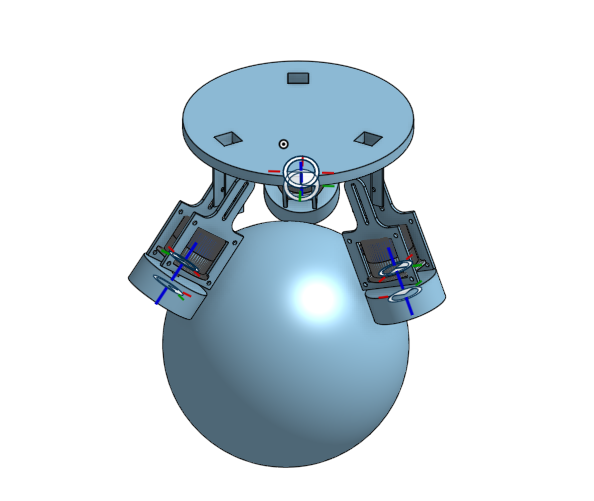
\includegraphics[width=\linewidth]{Metodologia/Figuras/ballbot.png}
        \caption{Modelo 3D}
        \label{fig:modelo_3D}
    \end{subfigure}
\end{figure}

O corpo do robô é um pequeno cilindro, onde são fixados os componentes eletrônicos. Além disso, possui partes que podem se mover para variar o ângulo das rodas e facilitar a acomodação. Essas partes também envolvem a fixação dos motores ao corpo.

\section{A modelagem matemática}
\label{sec:modelagemmatematica}

Para o projeto de controle, fez-se necessário realizar a modelagem mecânica do robô. A etapa seguinte relata como isso foi feito por meio da separação em planos 2D e obtenção das equações de movimento pelo cálculo do Lagrangiano e aplicação das equações de Euler-Lagrange. O passo a passo para realizar os cálculos foi semelhante ao presente no artigo \cite{phdthesis} e adaptado ao modelo projetado.

\subsection{Descrição do modelo}

O robô projetado foi um sistema tridimensional complexo formado por uma esfera, três rodas omnidirecionais e um corpo. Para a representação matemática simplificada, esse modelo foi dividido em três modelos planos independentes (Fig: \ref{fig:modelos_planos}).

\begin{figure}[H]
    \centering
    \begin{subfigure}[b]{0.4\textwidth}
        \centering
        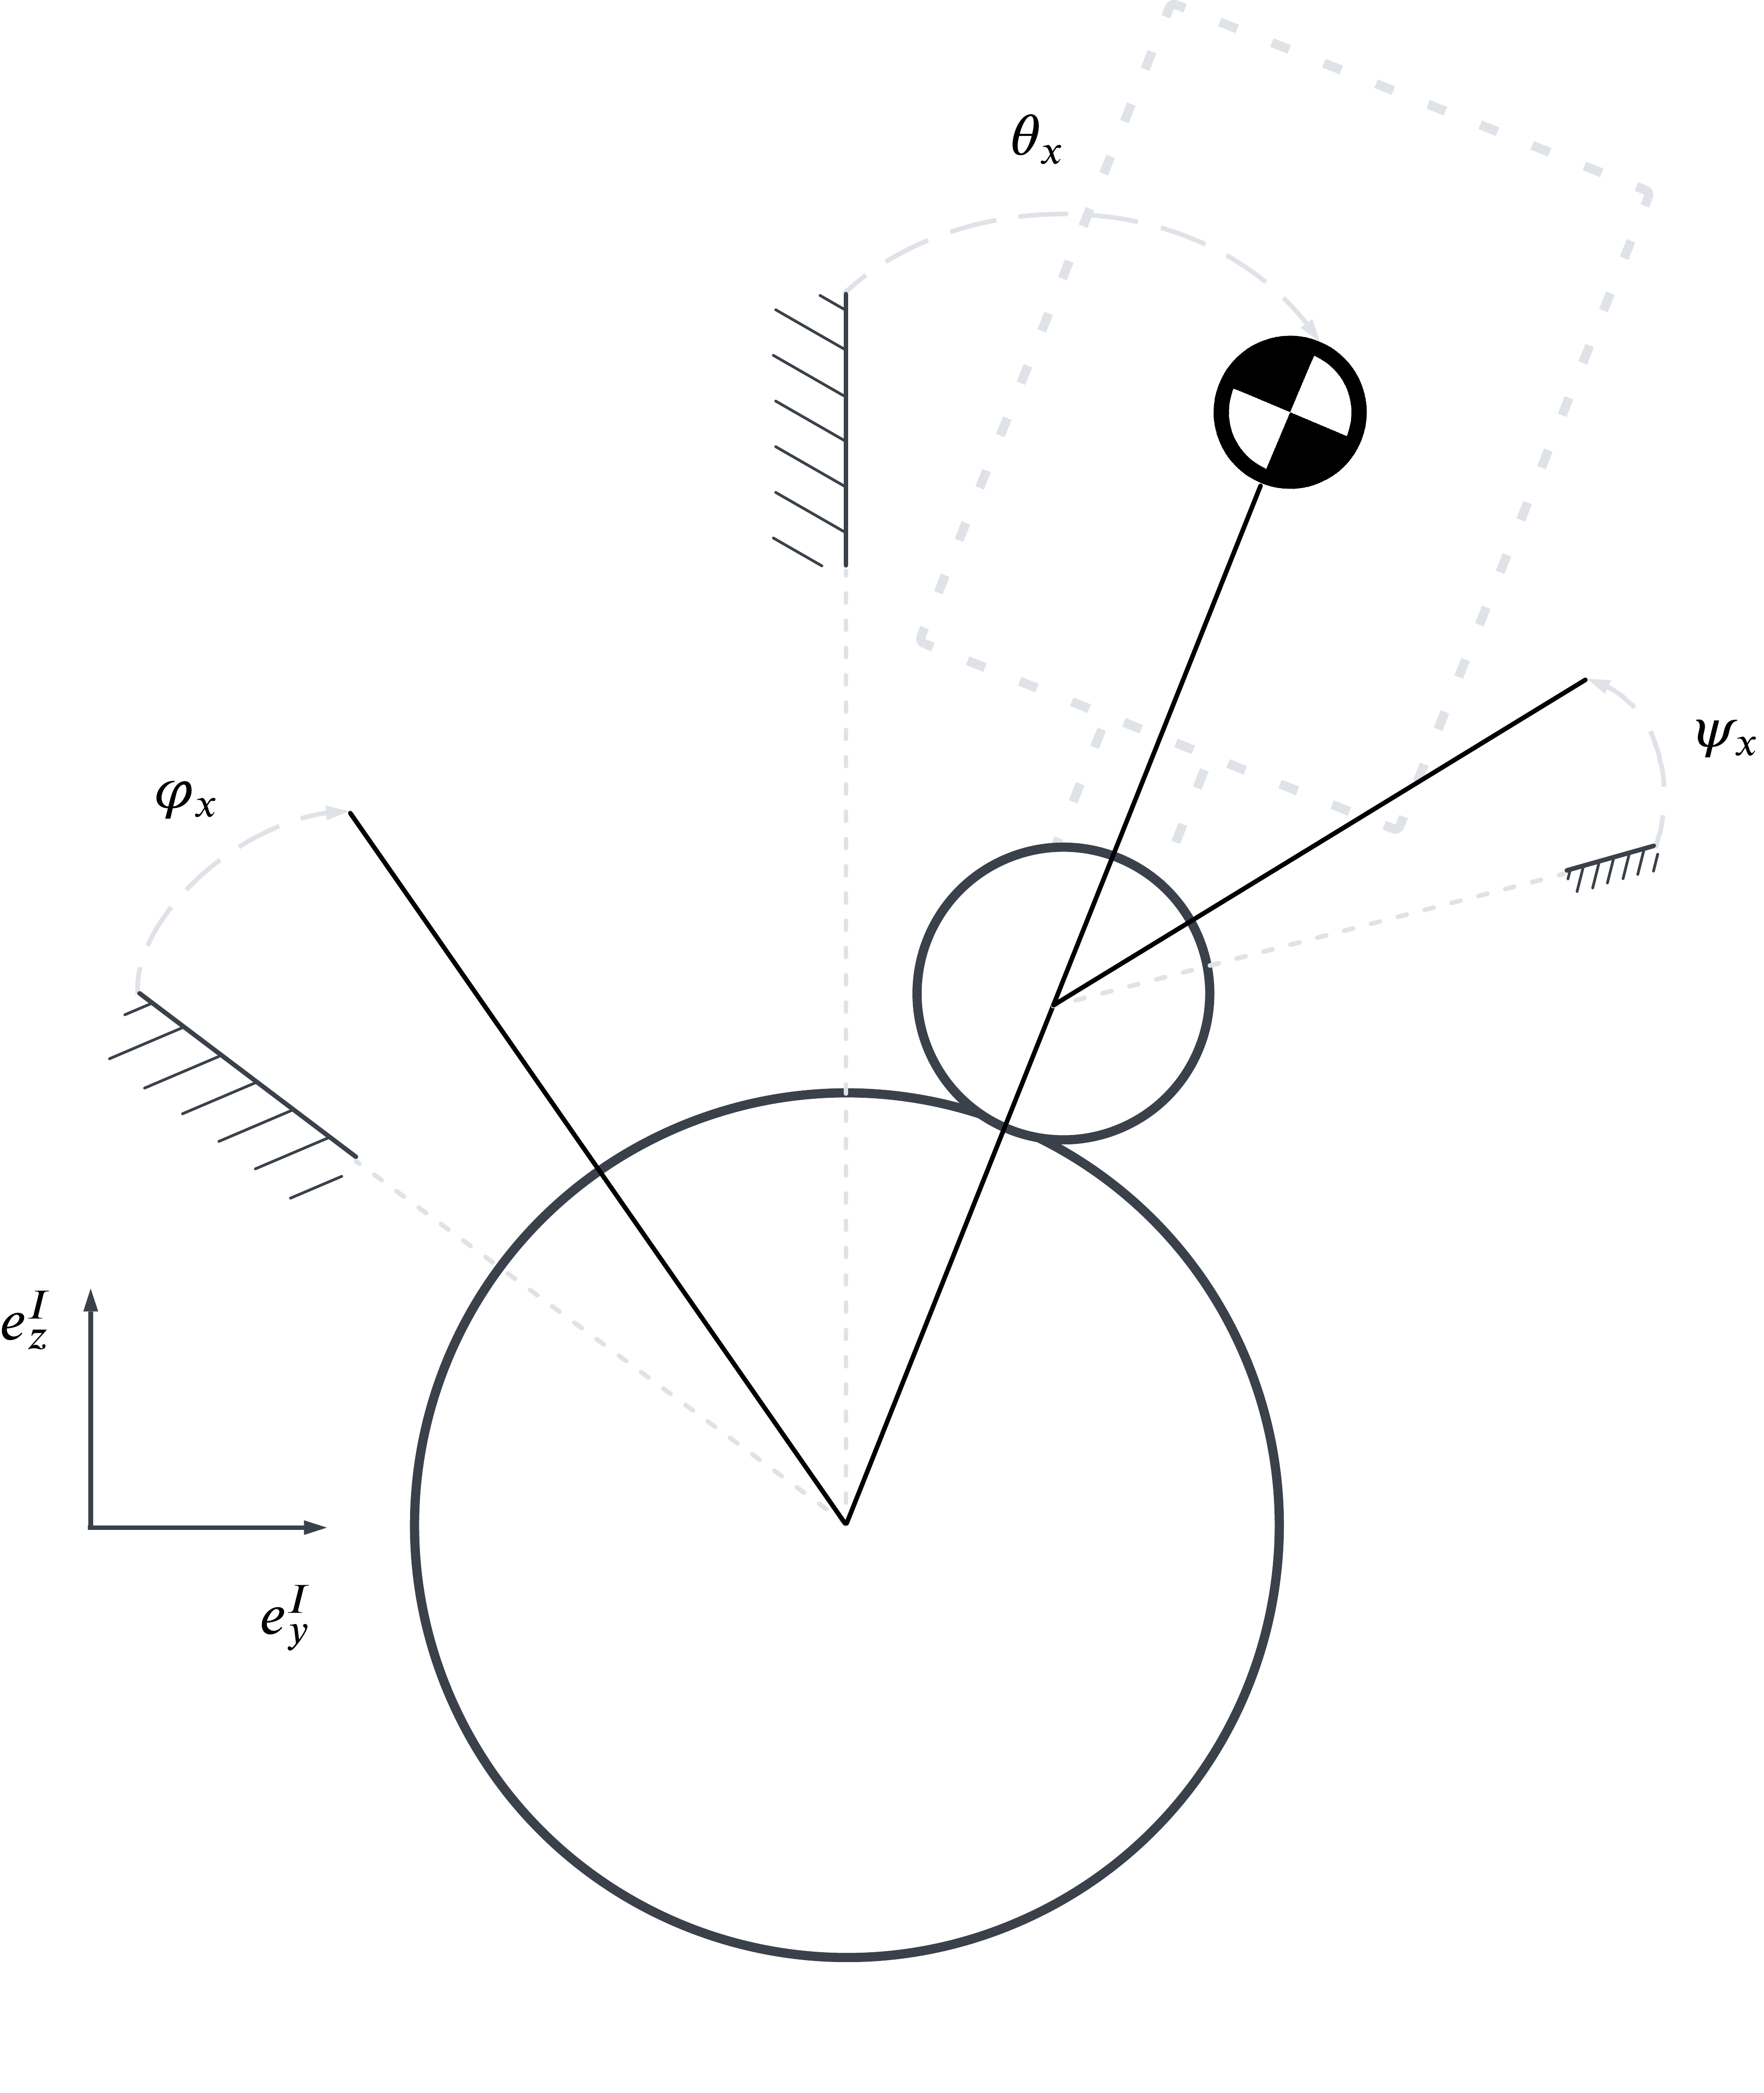
\includegraphics[width=\linewidth]{Metodologia/Figuras/modelo_plano_yz.png}
        \caption{Modelo no plano y-z}
        \label{fig:modelo_yz}
    \end{subfigure}
    \hfill
    \begin{subfigure}[b]{0.4\textwidth}
        \centering
        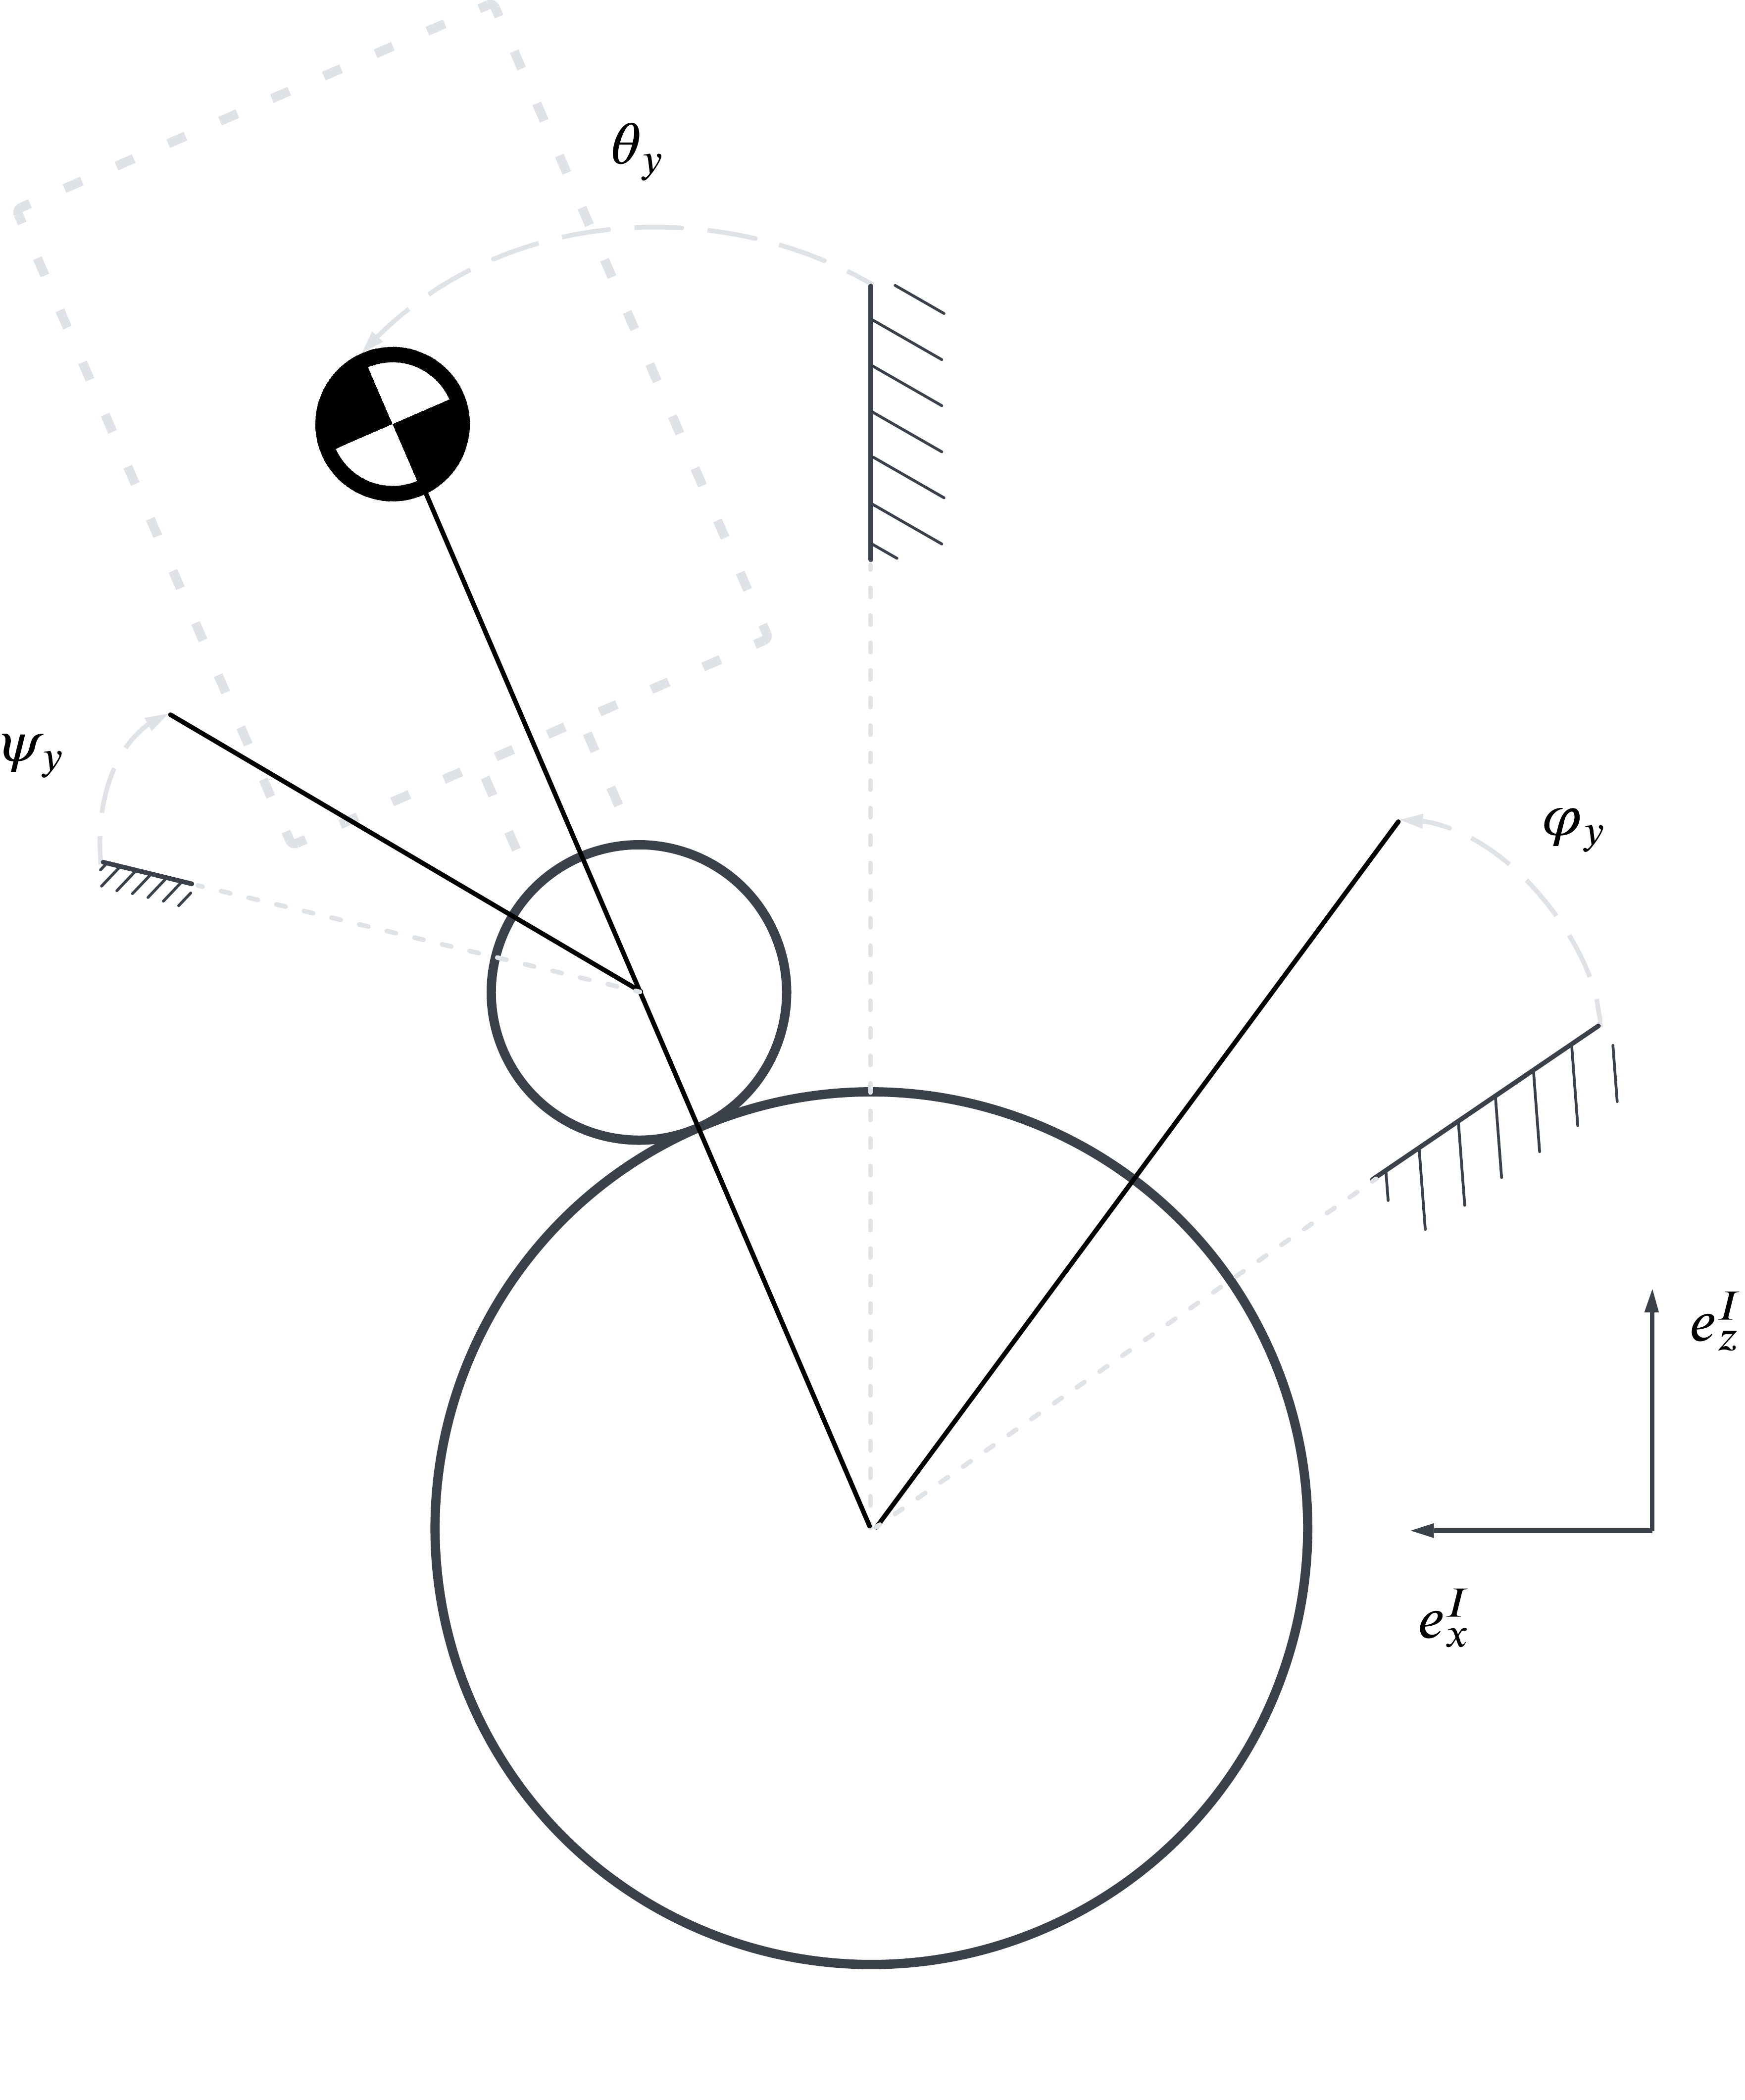
\includegraphics[width=\linewidth]{Metodologia/Figuras/modelo_plano_xz.png}
        \caption{Modelo no plano x-z}
        \label{fig:modelo_xz}
    \end{subfigure}
    \hfill
    \begin{subfigure}[b]{0.4\textwidth}
        \centering
        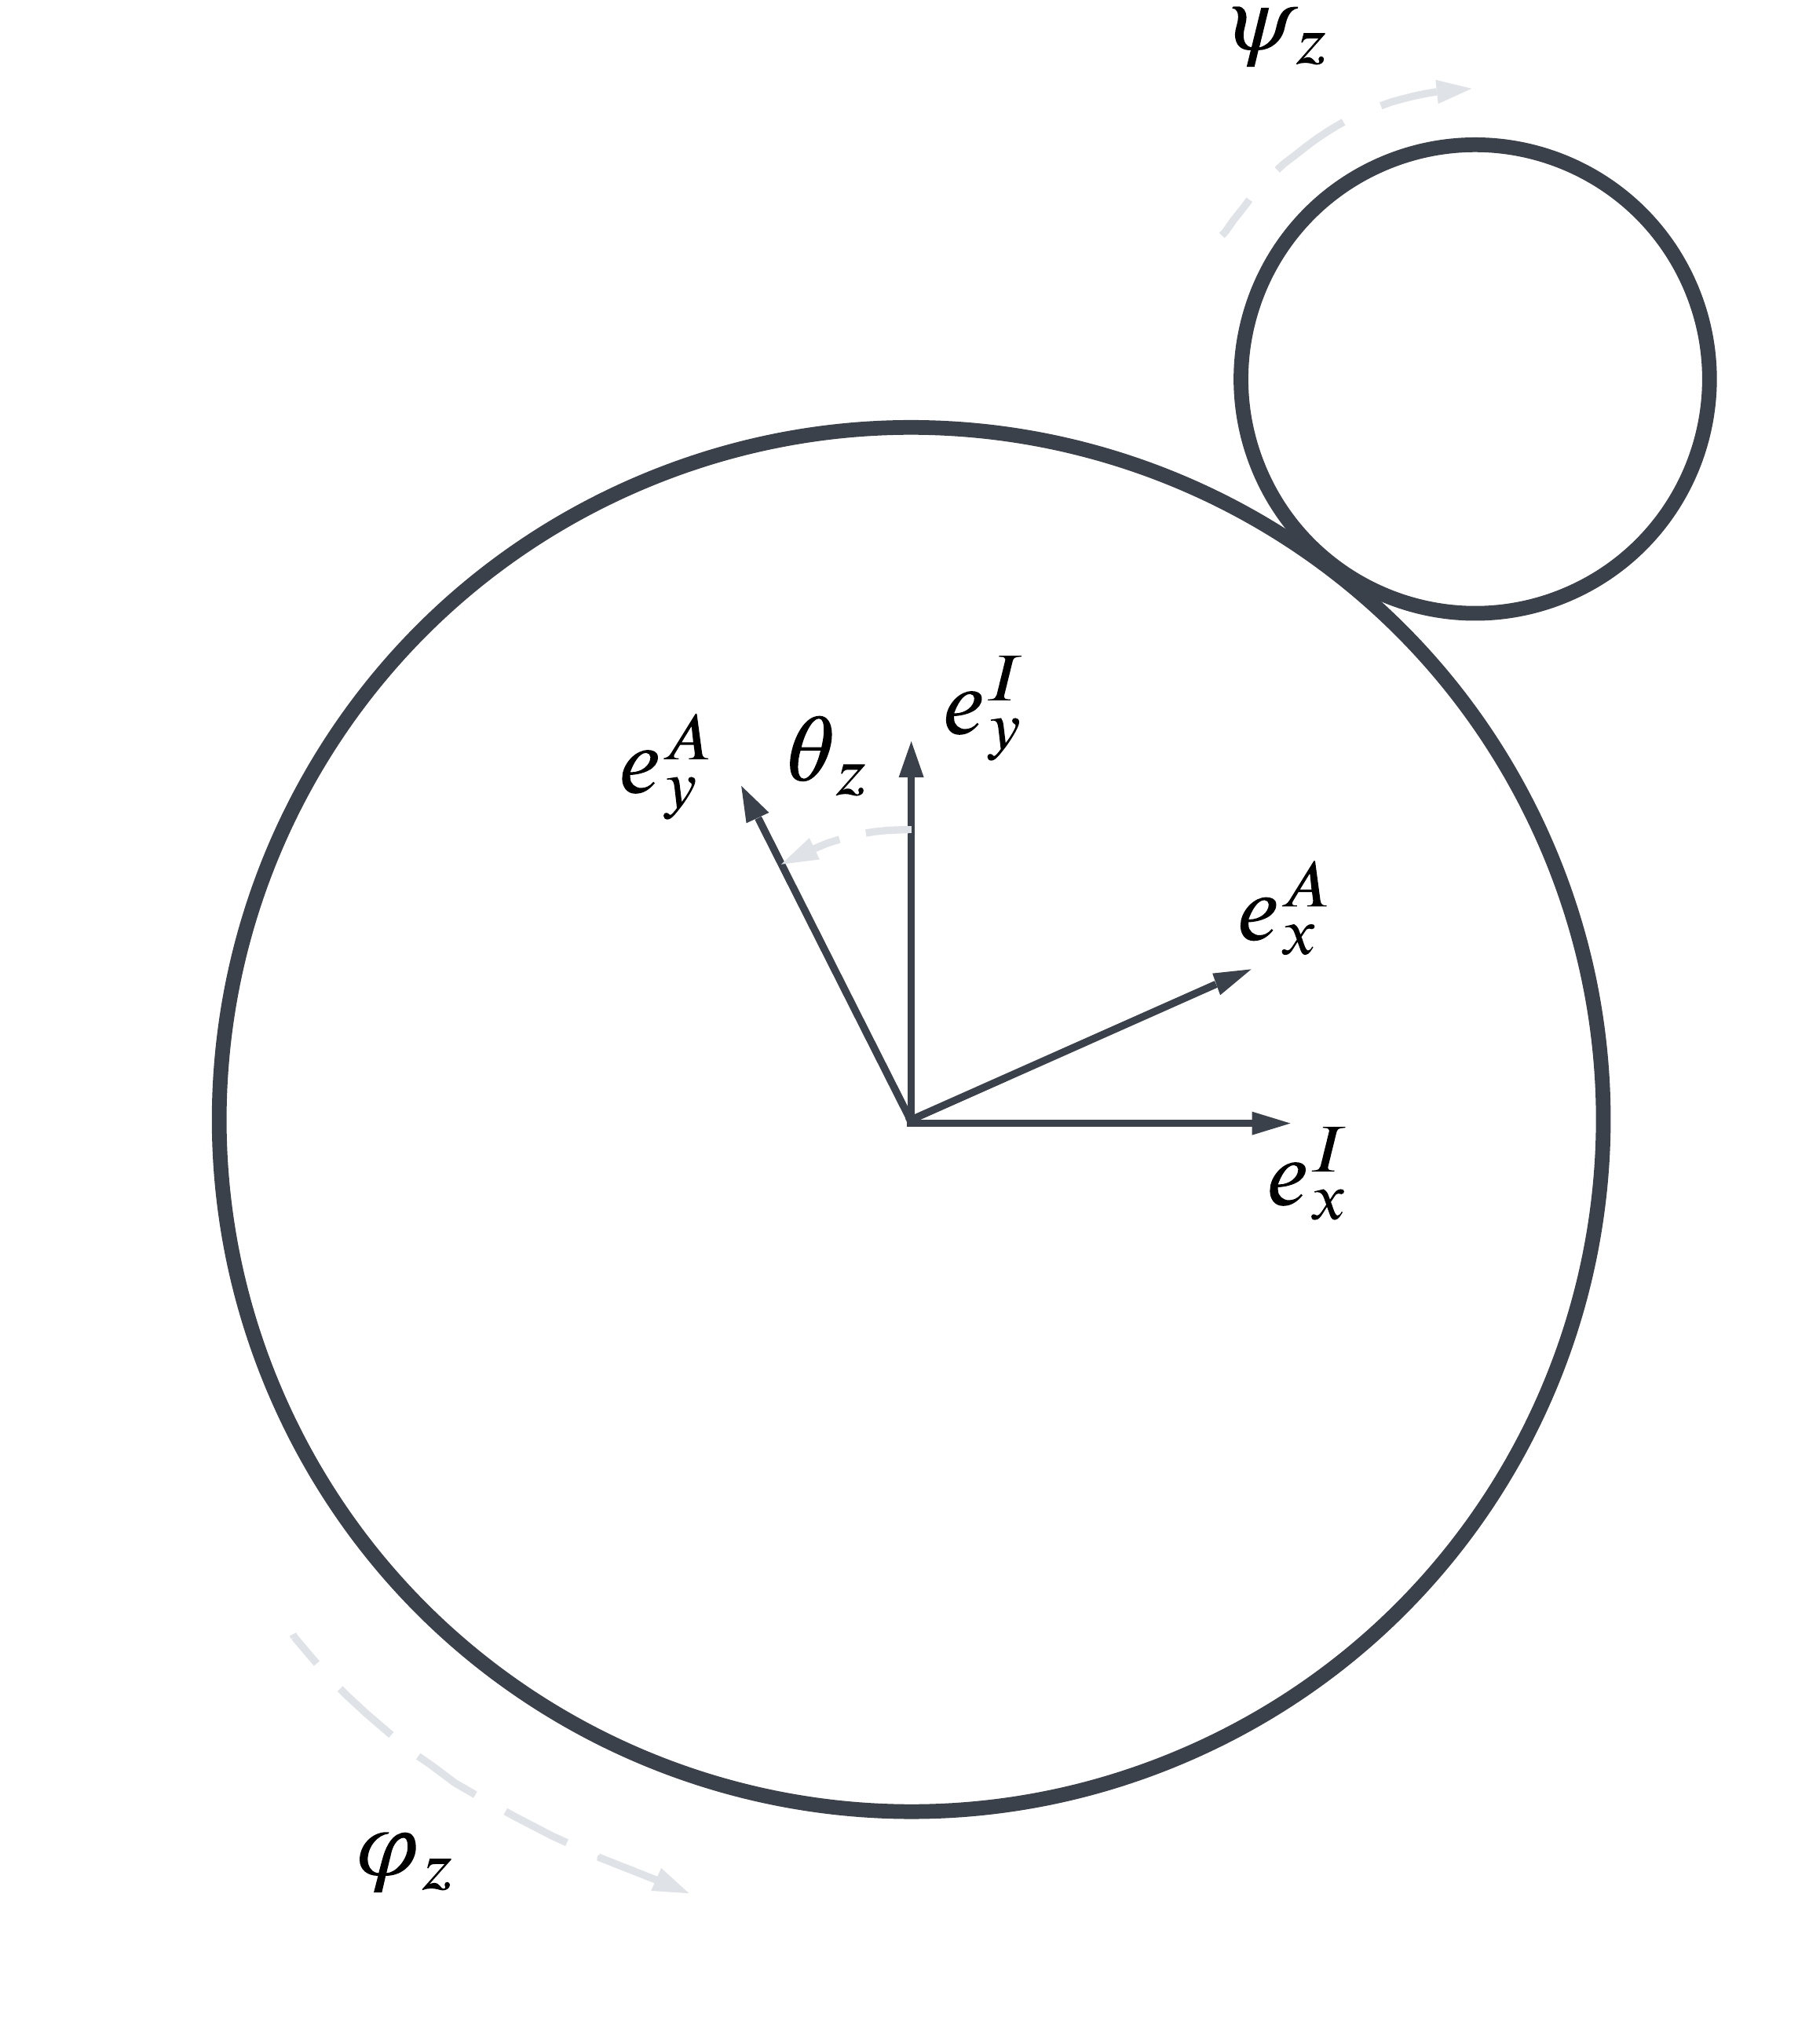
\includegraphics[width=\linewidth]{Metodologia/Figuras/modelo_plano_xy.png}
        \caption{Modelo no plano x-y}
        \label{fig:modelo_xy}
    \end{subfigure}
    \caption{Modelos nos diferentes planos}
    \label{fig:modelos_planos}
\end{figure}

Dessa forma, as três rodas omnidirecionais, que tinham o papel de movimentar o robô, foram transformadas em rodas virtuais, e cada uma foi representada em um modelo. Por causa dessa simplificação, posteriormente foram feitos cálculos para a conversão de posições e velocidades das rodas virtuais para as rodas reais.

\subsection{Suposições}

Os três modelos foram gerados a partir da subdivisão em planos do modelo tridimensional. Consequentemente, os efeitos de acoplamento entre eles foram desconsiderados. Nesse contexto, assumiu-se que o modelo representado no plano $y$-$z$ e o modelo representado no plano $x$-$z$ eram figuras espelhadas uma da outra. Por outro lado, o terceiro modelo, representado no plano $x$-$y$, tinha uma visão única, e apenas descrevia a rotação em torno do eixo \( z \) no sistema de coordenadas fixo do corpo (Fig: \ref{fig:modelo_xy}).

Ademais, com o intuito de simplificar ainda mais os cálculos e garantir a viabilidade do modelo matemático, foram adotadas as seguintes suposições:

\begin{itemize}
    \item Não há deslizamento entre a esfera e a superfície em que o robô está posicionado, assim como entre a esfera e as rodas omnidirecionais.
    \item Apenas o atrito em torno do eixo $z$, entre a esfera e a superfície, foi considerado. Todas as demais forças de atrito foram desconsideradas por serem consideradas irrelevantes.
    \item As interações entre os pontos de contato do robô são idealizadas, ou seja, não há deformações em nenhum desses pontos.
    \item A dinâmica dos motores é significativamente mais rápida do que a dinâmica de estabilização do robô, permitindo que a primeira seja tratada como praticamente instantânea em relação à segunda.
    \item A esfera está restrita a movimentos no plano horizontal, eliminando quaisquer componentes verticais.
\end{itemize}

\subsection{Parâmetros}

O robô possui alguns parâmetros estruturais que foram medidos e estão dispostos na tabela a seguir:

\begin{table}[H]
\centering
\begin{tabular}{|m{6cm}|c|c|c|}
\hline
Parâmetro & Símbolo  & Valor & Unidade de medida \\ \hline
Massa da esfera & $m_K$  & - & $kg$ \\ \hline
Massa da roda & $m_W$  & - & $kg$ \\ \hline
Massa do corpo & $m_A$  & - & $kg$ \\ \hline
Raio da esfera & $r_K$  & - & $m$ \\ \hline
Raio da roda & $r_W$  & - & $m$ \\ \hline
Distância entre o centro da esfera e o centro de massa do corpo & $l$ & - & $m$ \\ \hline
Momento de inércia da esfera & $\Theta_K$  & - & $kg \cdot m^2$ \\ \hline
Momento de inércia da roda nos planos $x$-$z$ e $y$-$z$ & $\Theta_W$  & - & $kg \cdot m^2$ \\ \hline
Momento de inércia da roda no plano $x$-$y$ & $\Theta_{W,xy}$  & - & $kg \cdot m^2$ \\ \hline
Momento de inércia do corpo & $\Theta_{A}$  & - & $kg \cdot m^2$ \\ \hline
Momento de inércia do corpo no plano $x$-$y$ & $\Theta_{A,xy}$  & - & $kg \cdot m^2$ \\ \hline
Ângulo entre o ponto de contato das rodas e o eixo z do sistema de coordenadas da esfera & $\alpha$  & - & $graus$ \\ \hline
Aceleração da gravidade & $g$  & $9,8$ & $\frac{m}{s^2}$ \\ \hline
\end{tabular}
\caption{Parâmetros estruturais}
\label{tab:tabela1}
\end{table}

\subsection{Coordenadas}

Cada um dos modelos foi completamente descrito utilizando os seguintes vetores de coordenadas mínimas:

\begin{equation}
\label{eq:1}
\begin{array}{ccc}
\vec{q_{xy}} =
\begin{bmatrix}
\varphi_z \\
\theta_z
\end{bmatrix}
& 
\vec{q_{yz}} =
\begin{bmatrix}
\varphi_x \\
\theta_x
\end{bmatrix}
& 
\vec{q_{xz}} =
\begin{bmatrix}
\varphi_y \\
\theta_y
\end{bmatrix}
\end{array}
\end{equation}

Onde:

\begin{itemize}
    \item $\varphi_{x,y,z}$: São as orientações da esfera;
    \item $\theta_{x,y,z}$: São as orientações do corpo;
    \item $\psi_{x,y,z}$: São os ângulos das rodas vituais.
\end{itemize}

\subsection{Equações de ligação}

Todas as coordenadas foram expressas utilizando os vetores de coordenadas mínimas e considerando a condição de rolamento sem deslizamento. Para um objeto circular que rola sem deslizar, o deslocamento linear do centro é diretamente proporcional à sua rotação angular, e pode ser calculado pela fórmula:

\begin{equation*}
    \begin{aligned}
        S = r \cdot \theta
    \end{aligned}
\end{equation*}

onde:

\begin{itemize}
    \item \( S \): Deslocamento linear do objeto, medido ao longo do caminho percorrido;
    \item \( r \): Raio do objeto circular;
    \item \( \theta \): Ângulo de rotação do objeto.
\end{itemize}

As coordenadas da esfera, da roda virtual e do centro de massa do corpo no plano $x$-$z$ foram definidas como:

\paragraph{Esfera:}

\begin{equation}
    \label{eq:2}
    \begin{aligned}
        x_K = r_K \cdot \varphi_y,
    \end{aligned}
\end{equation}

\begin{equation}
    \label{eq:3}
    \begin{aligned}
        z_K = 0.
    \end{aligned}
\end{equation}

\paragraph{Roda virtual:}

\begin{equation}
    \label{eq:4}
    \begin{aligned}
        x_W = (r_K \cdot \varphi_y) + (r_K + r_W) \cdot \sin{(\theta_y)},
    \end{aligned}
\end{equation}

\begin{equation}
    \label{eq:5}
    \begin{aligned}
        z_W = (r_K + r_W) \cdot \cos{(\theta_y)}.
    \end{aligned}
\end{equation}

\paragraph{Centro de massa do corpo:}

\begin{equation}
    \label{eq:6}
    \begin{aligned}
        x_A = (r_K \cdot \varphi_y) + l \cdot \sin{(\theta_y)},
    \end{aligned}
\end{equation}

\begin{equation}
    \label{eq:7}
    \begin{aligned}
        z_A = l \cdot \cos{(\theta_y)}.
    \end{aligned}
\end{equation}

Analogamente, foram encontradas as coordenadas no plano $y$-$z$:

\paragraph{Esfera:}

\begin{equation}
    \label{eq:8}
    \begin{aligned}
        y_K = r_K \cdot \varphi_x,
    \end{aligned}
\end{equation}

\begin{equation}
    \label{eq:9}
    \begin{aligned}
        z_K = 0.
    \end{aligned}
\end{equation}

\paragraph{Roda virtual:}

\begin{equation}
    \label{eq:10}
    \begin{aligned}
        y_W = (r_K \cdot \varphi_x) + (r_K + r_W) \cdot \sin{(\theta_x)},
    \end{aligned}
\end{equation}

\begin{equation}
    \label{eq:11}
    \begin{aligned}
        z_W = (r_K + r_W) \cdot \cos{(\theta_x)}.
    \end{aligned}
\end{equation}

\paragraph{Centro de massa do corpo:}

\begin{equation}
    \label{eq:12}
    \begin{aligned}
        y_A = (r_K \cdot \varphi_x) + l \cdot \sin{(\theta_x)},
    \end{aligned}
\end{equation}

\begin{equation}
    \label{eq:13}
    \begin{aligned}
        z_A = l \cdot \cos{(\theta_x)}.
    \end{aligned}
\end{equation}

No modelo do plano $x$-$z$, o ponto $A$ foi definido como o ponto de contato localizado na superfície da esfera, enquanto o ponto $B$ foi definido como o ponto de contato localizado na superfície da roda virtual. Suas velocidades, \( V_A \) e \( V_B \), foram assumidas iguais devido à condição de não deslizamento:

\begin{equation*}
    V_A = V_B \implies 
    \begin{bmatrix}
    V_{Ax} \\
    V_{Az}
    \end{bmatrix} = 
    \begin{bmatrix}
    V_{Bx} \\
    V_{Bz}
    \end{bmatrix}.
\end{equation*}

Substituindo-se os valores chegou-se em:

\begin{equation*}
    \begin{aligned}
        \begin{bmatrix}
        \dot x_K + \dot \varphi_y \cdot r_k \cdot \cos(\theta_y) \\
        \dot \varphi_y \cdot r_K \cdot \sin(\theta_y)
        \end{bmatrix}=
        \begin{bmatrix}
        \dot x_K + (r_K + r_W) \cdot \cos(\theta_y) \cdot \dot \theta_y + \dot \psi_y \cdot r_W \cdot \cos(\theta_y) \\
        - (r_K + r_W) \cdot \sin(\theta_y) \cdot \dot \theta_y + \dot \psi_y \cdot r_W \cdot \sin(\theta_y)
        \end{bmatrix}.
    \end{aligned}
\end{equation*}

Ao se isolar $\dot \psi_y$, obteve-se:

\begin{equation}
    \label{eq:14}
    \begin{aligned}
        \dot \psi_y = \frac{r_K}{r_W} \cdot (\dot \varphi_y - \dot \theta_y) - \dot \theta_y
    \end{aligned}.
\end{equation}

Analogamente, no plano $y$-$z$, foi obtido:

\begin{equation}
    \label{eq:15}
    \begin{aligned}
        \dot \psi_x = \frac{r_K}{r_W} \cdot (\dot \varphi_x - \dot \theta_x) - \dot \theta_x
    \end{aligned}.
\end{equation}

Por fim, utilizando-se o modelo no plano $x$-$y$, as velocidades \( V_A \) e \( V_B \) foram definidas como:

\begin{equation*}
    V_A = 
    \begin{bmatrix}
    V_{Ax} \\
    V_{Ay}
    \end{bmatrix}, \quad 
    V_B = 
    \begin{bmatrix}
    V_{Bx} \\
    V_{By}
    \end{bmatrix}.
\end{equation*}

Assumiu-se novamente \( V_A = V_B \) e se substituíram os valores, obtendo-se:

\begin{equation*}
    \begin{aligned}
        \begin{bmatrix}
        r_K \cdot \sin(\alpha) \cdot \dot \varphi_z \cdot \cos(\theta_z) \\
        r_K \cdot \sin(\alpha) \cdot \dot \varphi_z \cdot \sin(\theta_z)
        \end{bmatrix}=
        \begin{bmatrix}
        r_K \cdot \sin(\alpha) \cdot \dot \theta_z \cdot \cos(\theta_z) + r_W \cdot \dot \psi_z \cdot \cos(\theta_z)\\
        r_K \cdot \sin(\alpha) \cdot \dot \theta_z \cdot \sin(\theta_z) + r_W \cdot \dot \psi_z \cdot \sin(\theta_z)
        \end{bmatrix}.
    \end{aligned}
\end{equation*}

Isolando \( \dot{\psi}_z \), foi obtido:

\begin{equation}
    \label{eq:16}
    \begin{aligned}
        \dot \psi_z = \frac{r_K}{r_W} \cdot \sin(\alpha) \cdot (\dot \varphi_z - \dot \theta_z)
    \end{aligned}.
\end{equation}

\subsection{Energias}

O cálculo das energias potenciais e cinéticas é essencial para a modelagem utilizando o método de Euler-Lagrange. Portanto, para cada modelo planar, esses valores foram calculados como demonstrado a seguir.

\subsubsection{Plano y-z}

\paragraph{Esfera: Energia potencial}

O referencial escolhido se localizava no centro da esfera, logo, a energia potencial nessa situação era nula:

\begin{equation*}
    \begin{aligned}
        V_{K,yz} = 0
    \end{aligned}
\end{equation*}

\paragraph{Esfera: Energia cinética}

A energia cinética foi obtida por meio da soma da parte translacional e da parte rotacional:

\begin{equation*}
    \begin{aligned}
        T_{K,yz} & =\frac{1}{2} \cdot m_K \cdot (r_K \cdot \dot\varphi_x)^2 + \frac{1}{2} \cdot \Theta_K \cdot \dot\varphi_x^2
    \end{aligned}
\end{equation*}

\paragraph{Roda: Energia potencial}

\begin{equation*}
    \begin{aligned}
        V_{W,yz} & = m_W \cdot g \cdot (r_K + r_W) \cdot \cos{(\theta_x)}
    \end{aligned}
\end{equation*}

\paragraph{Roda: Energia cinética}

\begin{equation*}
    \begin{aligned}
        T_{W,yz} & = \frac{1}{2} \cdot m_W \cdot 
        \begin{bmatrix}
            \dot x_W \\
            \dot y_W \\
            \dot z_W
        \end{bmatrix}^T
        \cdot
        \begin{bmatrix}
            \dot x_W \\
            \dot y_W \\
            \dot z_W
        \end{bmatrix}
        +
        \frac{1}{2} \cdot \Theta_W \cdot \dot {\psi_x}^2
    \end{aligned}
\end{equation*}

Os valores de $x_W$, $y_W$ e $z_W$ são:

\begin{equation*}
\scalebox{0.85}{$
    \begin{aligned}
        \begin{bmatrix}
            x_W \\
            y_W \\
            z_W
        \end{bmatrix} 
        & =
        \begin{bmatrix}
            0 \\
            (\varphi_x \cdot r_K ) + (r_K + r_W) \cdot \sin(\theta_x) \\
            (r_K + r_W) \cdot \cos(\theta_x)
        \end{bmatrix}
        \implies
        \begin{bmatrix}
            \dot x_W \\
            \dot y_W \\
            \dot z_W
        \end{bmatrix}
        & =
        \begin{bmatrix}
            0 \\
            (\dot \varphi_x \cdot r_K ) + (r_K + r_W) \cdot \cos({\theta_x}) \cdot \dot \theta_x \\
            - (r_K + r_W) \cdot \sin({\theta_x}) \cdot \dot \theta_x
        \end{bmatrix}.
    \end{aligned}
    $}
\end{equation*}.

Ao substituir esse resultado na equação anterior, obteve-se:

\begin{equation*}
    \scalebox{0.65}{$
        \begin{aligned}
            T_{W,yz} = \frac{1}{2} \cdot m_W \cdot \Big[ (\dot{\varphi}_x \cdot r_K)^2 + 2 \cdot (\dot{\varphi}_x \cdot r_K) \cdot (r_K + r_W) \cdot \cos(\theta_x) \cdot \dot{\theta}_x + (r_K + r_W)^2 \cdot \dot{\theta}_x^2 \Big] + \frac{1}{2} \cdot \Theta_W \cdot \bigg(\frac{r_K}{r_W} \cdot (\dot{\varphi}_x - \dot{\theta}_x) - \dot{\theta}_x \bigg)^2
        \end{aligned}
    $}
\end{equation*}


\paragraph{Corpo: Energia potencial}

\begin{equation*}
    \begin{aligned}
        V_{A,yz} & = m_A \cdot g \cdot l \cdot \cos{(\theta_x)}
    \end{aligned}
\end{equation*}

\paragraph{Corpo: Energia cinética}

\begin{equation*}
    \begin{aligned}
        T_{A,yz} & = \frac{1}{2} \cdot m_A \cdot 
        \begin{bmatrix}
            \dot x_A \\
            \dot y_A \\
            \dot z_A
        \end{bmatrix}^T
        \cdot
        \begin{bmatrix}
            \dot x_A \\
            \dot y_A \\
            \dot z_A
        \end{bmatrix}
        +
        \frac{1}{2} \cdot \Theta_A \cdot \dot {\theta_x}^2
    \end{aligned}
\end{equation*}

Os valores de $x_A$, $y_A$ e $z_A$ são:

\begin{equation*}
    \begin{aligned}
        \begin{bmatrix}
            x_A \\
            y_A \\
            z_A
        \end{bmatrix} 
        & =
        \begin{bmatrix}
            0 \\
            (\varphi_x \cdot r_K ) + l \cdot \sin(\theta_x) \\
            l \cdot \cos(\theta_x)
        \end{bmatrix}
        \implies
        \begin{bmatrix}
            \dot x_A \\
            \dot y_A \\
            \dot z_A
        \end{bmatrix}
        & =
        \begin{bmatrix}
            0 \\
            (\dot \varphi_x \cdot r_K ) + l \cdot \cos({\theta_x}) \cdot \dot \theta_x \\
            - l \cdot \sin({\theta_x}) \cdot \dot \theta_x
        \end{bmatrix}.
    \end{aligned}
\end{equation*}.

Ao substituir esse resultado na equação anterior, foi obtido:

\begin{equation*}
    \begin{aligned}
        T_{A,yz} = \frac{1}{2} \cdot m_A \cdot \Big[ (\dot{\varphi}_x \cdot r_K)^2 + 2 \cdot (\dot{\varphi}_x \cdot r_K) \cdot l \cdot \cos(\theta_x) \cdot \dot{\theta}_x + l^2 \cdot \dot{\theta}_x^2 \Big] + \frac{1}{2} \cdot \Theta_A \cdot \dot \theta_x^2
    \end{aligned}
\end{equation*}

\subsubsection{Plano x-z}

As equações do plano x-z são análogas às equações do plano y-z.

\paragraph{Esfera: Energia potencial}

\begin{equation*}
    \begin{aligned}
        V_{K,xz} = 0
    \end{aligned}
\end{equation*}

\paragraph{Esfera: Energia cinética}

\begin{equation*}
    \begin{aligned}
        T_{K,xz} & = \frac{1}{2} \cdot m_K \cdot (r_K \cdot \dot\theta_y)^2 + \frac{1}{2} \cdot \Theta_K \cdot \dot\theta_y^2
    \end{aligned}
\end{equation*}

\paragraph{Roda: Energia potencial}

\begin{equation*}
    \begin{aligned}
        V_{W,xz} & = m_W \cdot g \cdot (r_K + r_W) \cdot \cos{(\theta_y)}
    \end{aligned}
\end{equation*}

\paragraph{Roda: Energia cinética}

\begin{equation*}
    \scalebox{0.65}{$
    \begin{aligned}
        T_{W,xz} = \frac{1}{2} \cdot m_W \cdot \Big[ (\dot{\varphi}_y \cdot r_K)^2 
        + 2 \cdot (\dot{\varphi}_y \cdot r_K) \cdot (r_K + r_W) \cdot \cos(\theta_y) \cdot \dot{\theta}_y + (r_K + r_W)^2 \cdot \dot{\theta}_y^2 \Big] + \frac{1}{2} \cdot \Theta_W \cdot \bigg(\frac{r_K}{r_W} \cdot (\dot{\varphi}_y - \dot{\theta}_y) - \dot{\theta}_y \bigg)^2
    \end{aligned}
    $}
\end{equation*}

\paragraph{Corpo: Energia potencial}

\begin{equation*}
    \begin{aligned}
        V_{A,xz} & = m_A \cdot g \cdot l \cdot \cos{(\theta_y)}
    \end{aligned}
\end{equation*}

\paragraph{Corpo: Energia cinética}

\begin{equation*}
    \begin{aligned}
        T_{A,xz} = \frac{1}{2} \cdot m_A \cdot \Big[ (\dot{\varphi}_y \cdot r_K)^2 + 2 \cdot (\dot{\varphi}_y \cdot r_K) \cdot l \cdot \cos(\theta_y) \cdot \dot{\theta}_y + l^2 \cdot \dot{\theta}_y^2 \Big] + \frac{1}{2} \cdot \Theta_A \cdot \dot \theta_y^2
    \end{aligned}
\end{equation*}

\subsubsection{Plano x-y}

\paragraph{Esfera: Energia cinética}

\begin{equation*}
    \begin{aligned}
        T_{K,xy} & = \frac{1}{2} \cdot \Theta_K \cdot \dot {\varphi_z}^2 
    \end{aligned}
\end{equation*}

\paragraph{Roda: Energia cinética}

\begin{equation*}
    \begin{aligned}
        T_{W,xy} & = \frac{1}{2} \cdot \Theta_{W,xy} \cdot \dot {\psi_z}^2 
    \end{aligned}
\end{equation*}

\paragraph{Corpo: Energia cinética}

\begin{equation*}
    \begin{aligned}
        T_{A,xy} & = \frac{1}{2} \cdot \Theta_{A,xy} \cdot \dot {\theta_z}^2 
    \end{aligned}
\end{equation*}

\subsection{Torques externos}

As forças não-potenciais \( \vec{f}_{NP} \) representam as forças externas atuando em um sistema. Neste caso, o torque do motor \( T_x \), ou seja, a entrada do sistema, é uma força não potencial. O torque do motor afeta diretamente a coordenada \( \psi_x \). Usando a equação \ref{eq:15}, o efeito do torque do motor nas coordenadas mínimas pode ser expresso como:

\begin{equation}
\label{eq:17}
\vec{f}_{NP,yz1} = 
\begin{bmatrix}
\frac{r_K}{r_W} \cdot T_x \\
-\left(1 + \frac{r_K}{r_W}\right) T_x
\end{bmatrix}
\end{equation}

O torque oposto que atua na coordenada \( \vartheta_x \) do corpo é expresso como:

\begin{equation}
\label{eq:18}
\vec{f}_{NP,yz2} =
\begin{bmatrix}
0 \\
T_x
\end{bmatrix}
\end{equation}

A força total não potencial é então a soma de \( \vec{f}_{NP,yz1} \) e \( \vec{f}_{NP,yz2} \). Um procedimento semelhante é aplicado no plano \( x \)-\( y \). Neste modelo, uma força adicional de atrito \( T_f \) atua em \( \varphi_z \), assim como na rotação da bola:

\begin{equation}
\label{eq:19}
\vec{f}_{NP,xy} =
\begin{bmatrix}
-T_f + \frac{r_K}{r_W} \sin{\alpha} \cdot T_z \\
-\frac{r_K}{r_W} \sin{\alpha} \cdot T_z + T_z
\end{bmatrix}
\end{equation}

\subsection{Equações de movimento}

\begin{equation*}
    \frac{d}{dt} \left( \frac{\partial T}{\partial \dot{\vec{q}}} \right)^T - \left( \frac{\partial T}{\partial \vec{q}} \right)^T + \left( \frac{\partial V}{\partial \vec{q}} \right)^T - \vec{f}_{NP} = 0.
\end{equation*}

$T$ e $V$ são, respectivamente, as energias cinéticas e as energias potenciais.

\begin{equation*}
    T = T_K + T_W + T_A
\end{equation*}
\begin{equation*}
    V = V_K + V_W + V_A
\end{equation*}

As equações de movimento do plano $y$-$z$ podem ser escritas na forma matricial.

\begin{equation*}
M_x(\vec{q}, \dot{\vec{q}}) \ddot{\vec{q}} + C_x(\vec{q}, \dot{\vec{q}}) + G_x(\vec{q}) = f_{NP}
\end{equation*}

As matrizes de inércia, $M_x$, de forças de Coriolis, $C_x$, e de forças gravitacionais, $G_x$, são:

\begin{equation*}
    \begin{aligned}
    M_x &= 
    \begin{bmatrix}
    m_{\text{tot}} r_K^2 + \Theta_K + \left( \frac{r_K}{r_W} \right)^2 \Theta_W & -\frac{r_K}{r_W^2} r_{\text{tot}} \Theta_W + \gamma r_K \cos \vartheta_x \\
    -\frac{r_K}{r_W^2} r_{\text{tot}} \Theta_W + \gamma r_K \cos \vartheta_x & \frac{r_{\text{tot}}^2}{r_W^2} \Theta_W + \Theta_A + m_A l^2 + m_W r_{\text{tot}}^2
    \end{bmatrix}
    \\
    C_x &= 
    \begin{bmatrix}
    -r_K \gamma \sin \vartheta_x \dot{\vartheta}_x^2 \\
    0
    \end{bmatrix}
    \\
    G_x &= 
    \begin{bmatrix}
    0 \\
    -g \sin \vartheta_x \gamma
    \end{bmatrix}
    \end{aligned}
\end{equation*}

Onde:

\begin{equation*}
    \begin{aligned}
        m_{\text{tot}} &= m_K + m_A + m_W \\
        r_{\text{tot}} &= r_K + r_W \\
        \gamma &= l \cdot m_A + (r_K + r_W) m_W
    \end{aligned}
\end{equation*}

A resolução das equações de Lagrange no plano $x$-$y$ para as coordenadas $\ddot{\varphi}_z$ e $\ddot{\vartheta}_z$ produziu:

\begin{equation}
    \label{eq:17}
    \begin{aligned}
    \ddot{\varphi}_z &= 
    -\frac{
    \left( r_W^2 \Theta_{A,xy} + r_K^2 \Theta_{W,xy} \sin^2 \alpha \right) \cdot T_f + r_K r_W \Theta_{A,xy} \sin \alpha \cdot T_z
    }{
    r_W^2 \Theta_{A,xy} \Theta_K + r_K^2 \left( \Theta_{A,xy} + \Theta_K \right) \Theta_{W,xy} \sin^2 \alpha
    }
    \end{aligned}
\end{equation}

\begin{equation}
    \label{eq:18}
    \begin{aligned}
    \ddot{\vartheta}_z &= 
    -\frac{
    r_K \sin \alpha \left( r_K \Theta_{W,xy} \sin \alpha \cdot T_f + r_W \Theta_K \cdot T_z \right)
    }{
    r_W^2 \Theta_{A,xy} \Theta_K + r_K^2 \left( \Theta_{A,xy} + \Theta_K \right) \Theta_{W,xy} \sin^2 \alpha
    }
    \end{aligned}
\end{equation}

Para determinar a força de atrito, considerou-se que a bola permanece constantemente aderida ao solo, satisfazendo a condição de aderência $\ddot\varphi=0$. Assim, com base na equação \ref{eq:17}, $T_f$ foi expresso da seguinte maneira:

\begin{equation*}
    T_f = \frac{r_K r_W \Theta_{A,xy} \sin \alpha \cdot T_z}{r_W^2 \Theta_{A,xy} + r_K^2 \Theta_{W,xy} \sin^2 \alpha}
\end{equation*}

\subsection{Conversão de torques}

Os modelos planares utilizam uma roda virtual para atuar no sistema. O sistema real possui uma estrutura de atuação que difere significativamente daquela assumida no modelo planar. Como um controlador projetado para o modelo planar será implementado no sistema real, é necessário calcular conversões. Para que seja possível controlar o sistema real, os torques nos motores virtuais devem ser convertidos nos torques dos motores reais.

A visão lateral e a visão superior do modelo real estão definidas nas figuras abaixo:

\begin{figure}[H]
    \centering
    \begin{subfigure}[b]{0.4\textwidth}
        \centering
        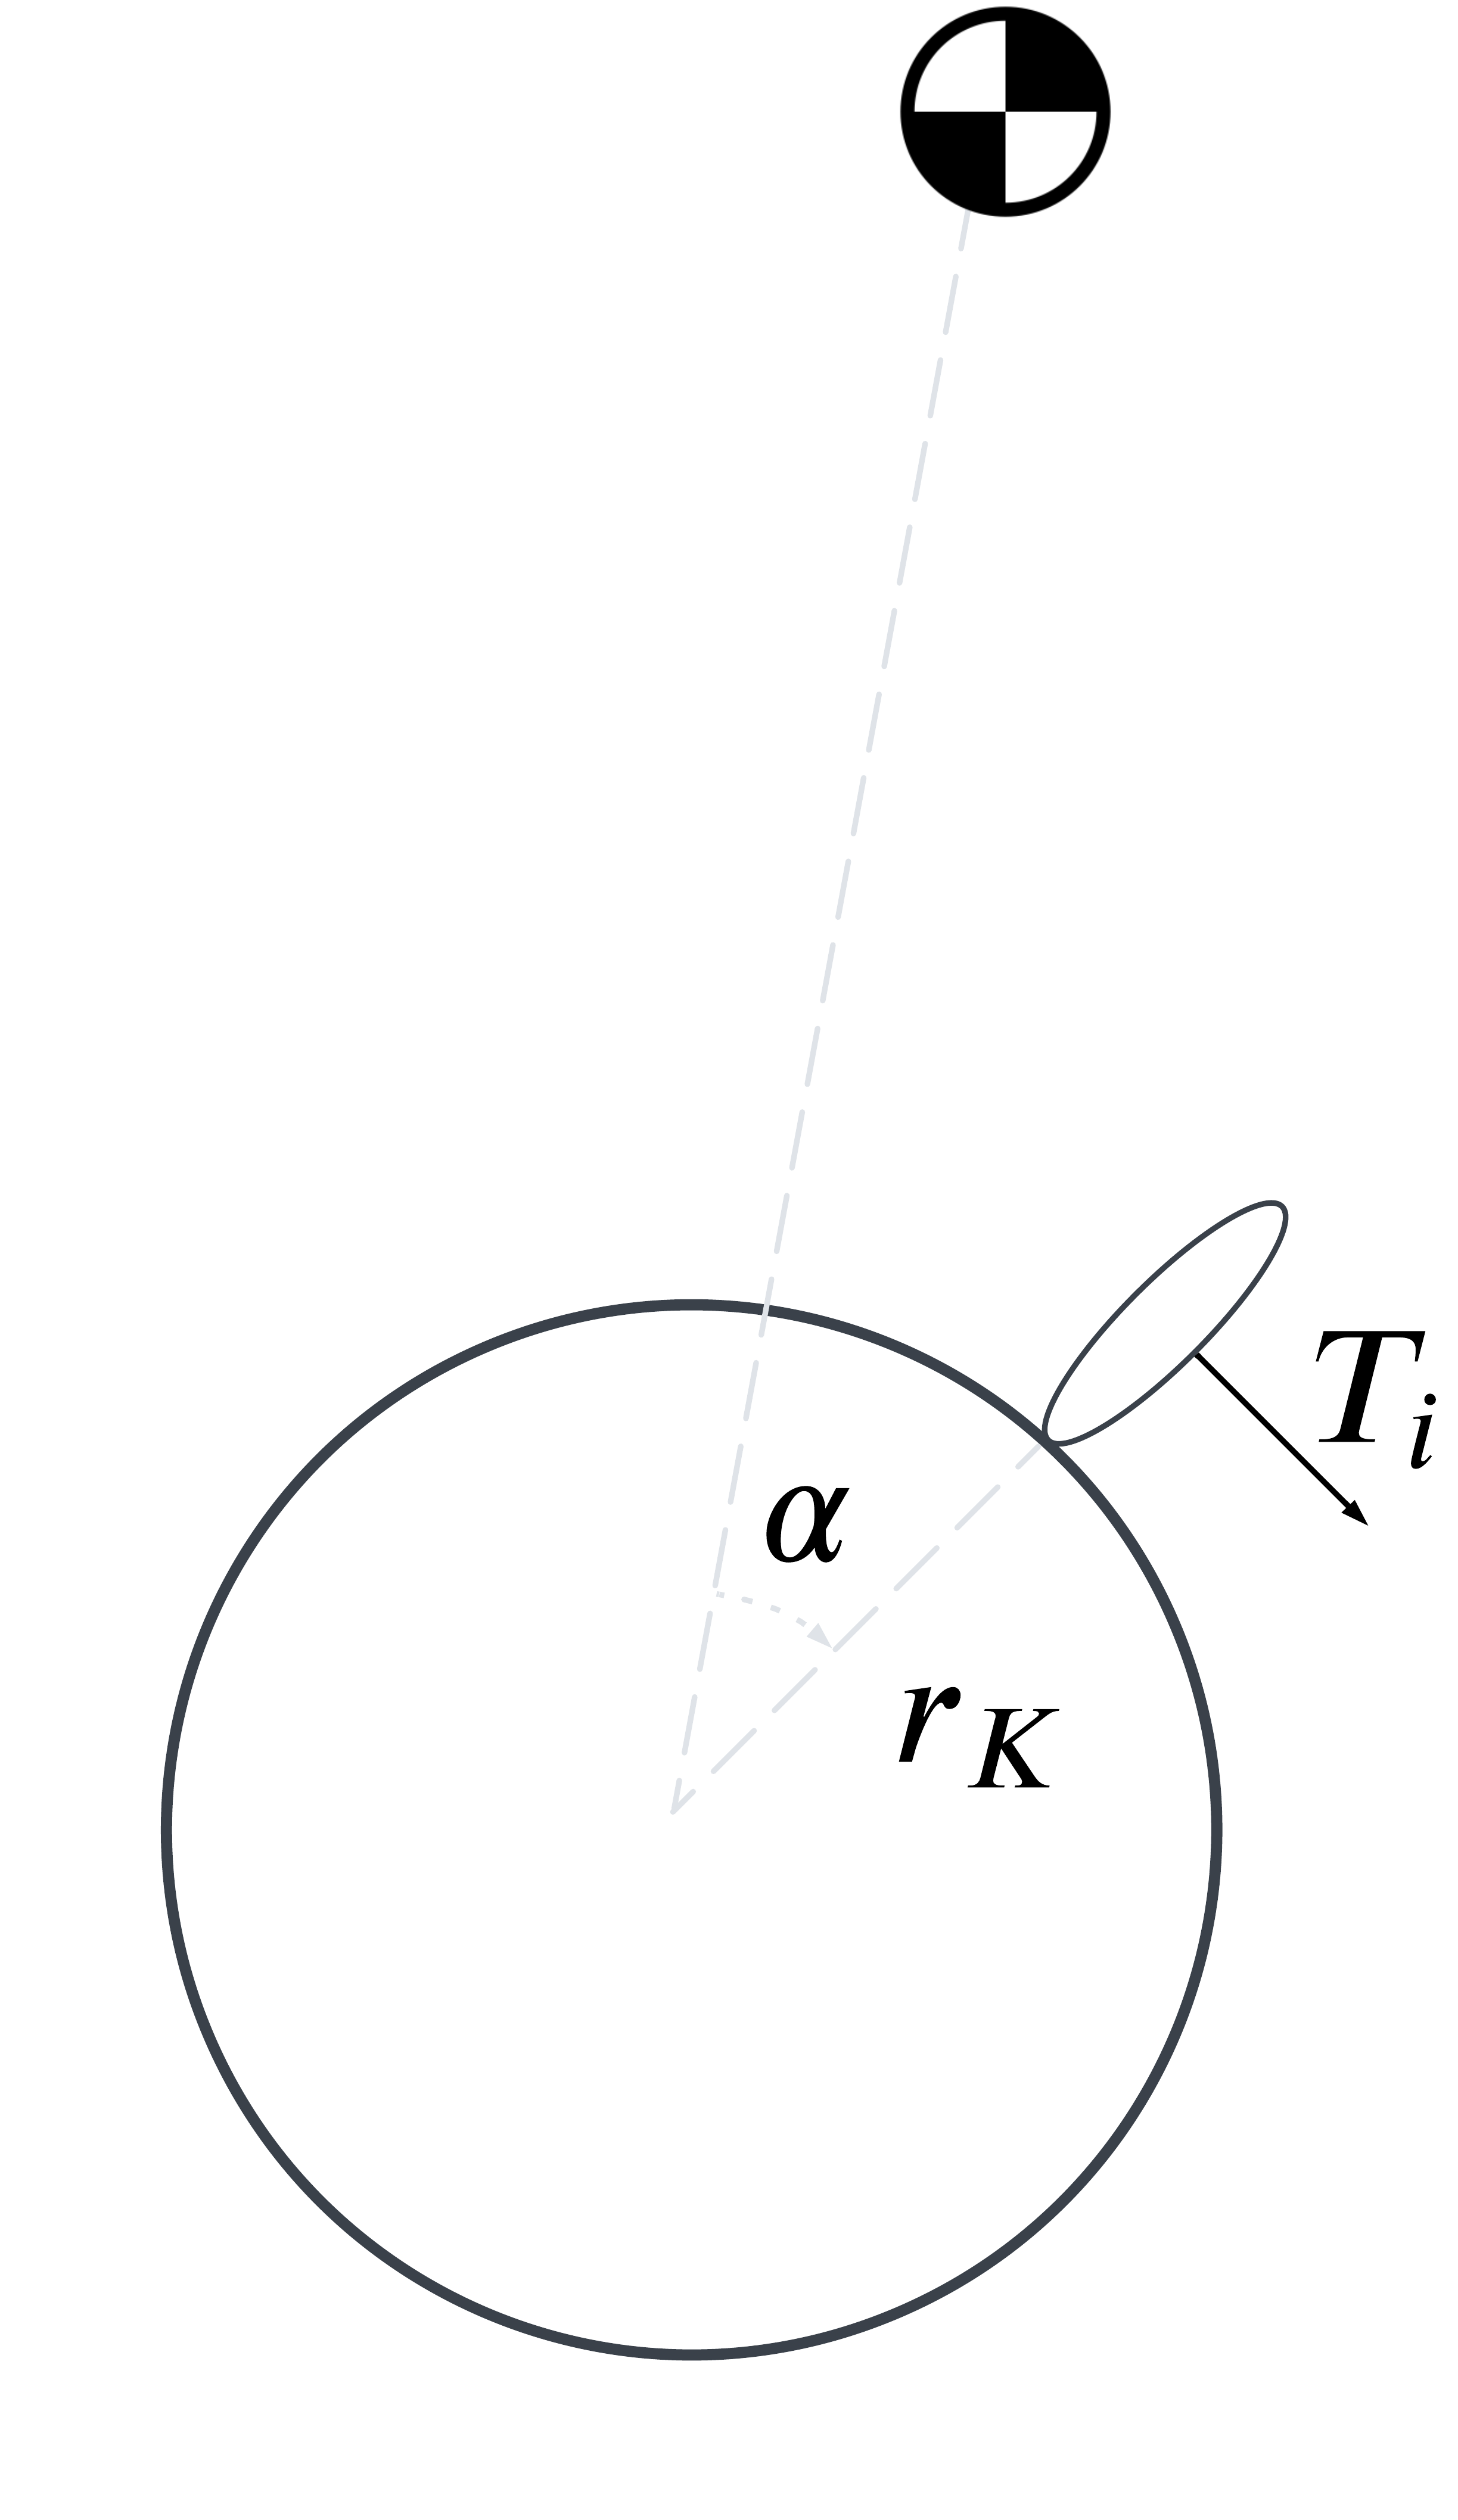
\includegraphics[width=\linewidth]{Metodologia/Figuras/torque_side.png}
        \caption{Modelo real visto de lado}
        \label{fig:torques_lado}
    \end{subfigure}
    \hfill
    \begin{subfigure}[b]{0.4\textwidth}
        \centering
        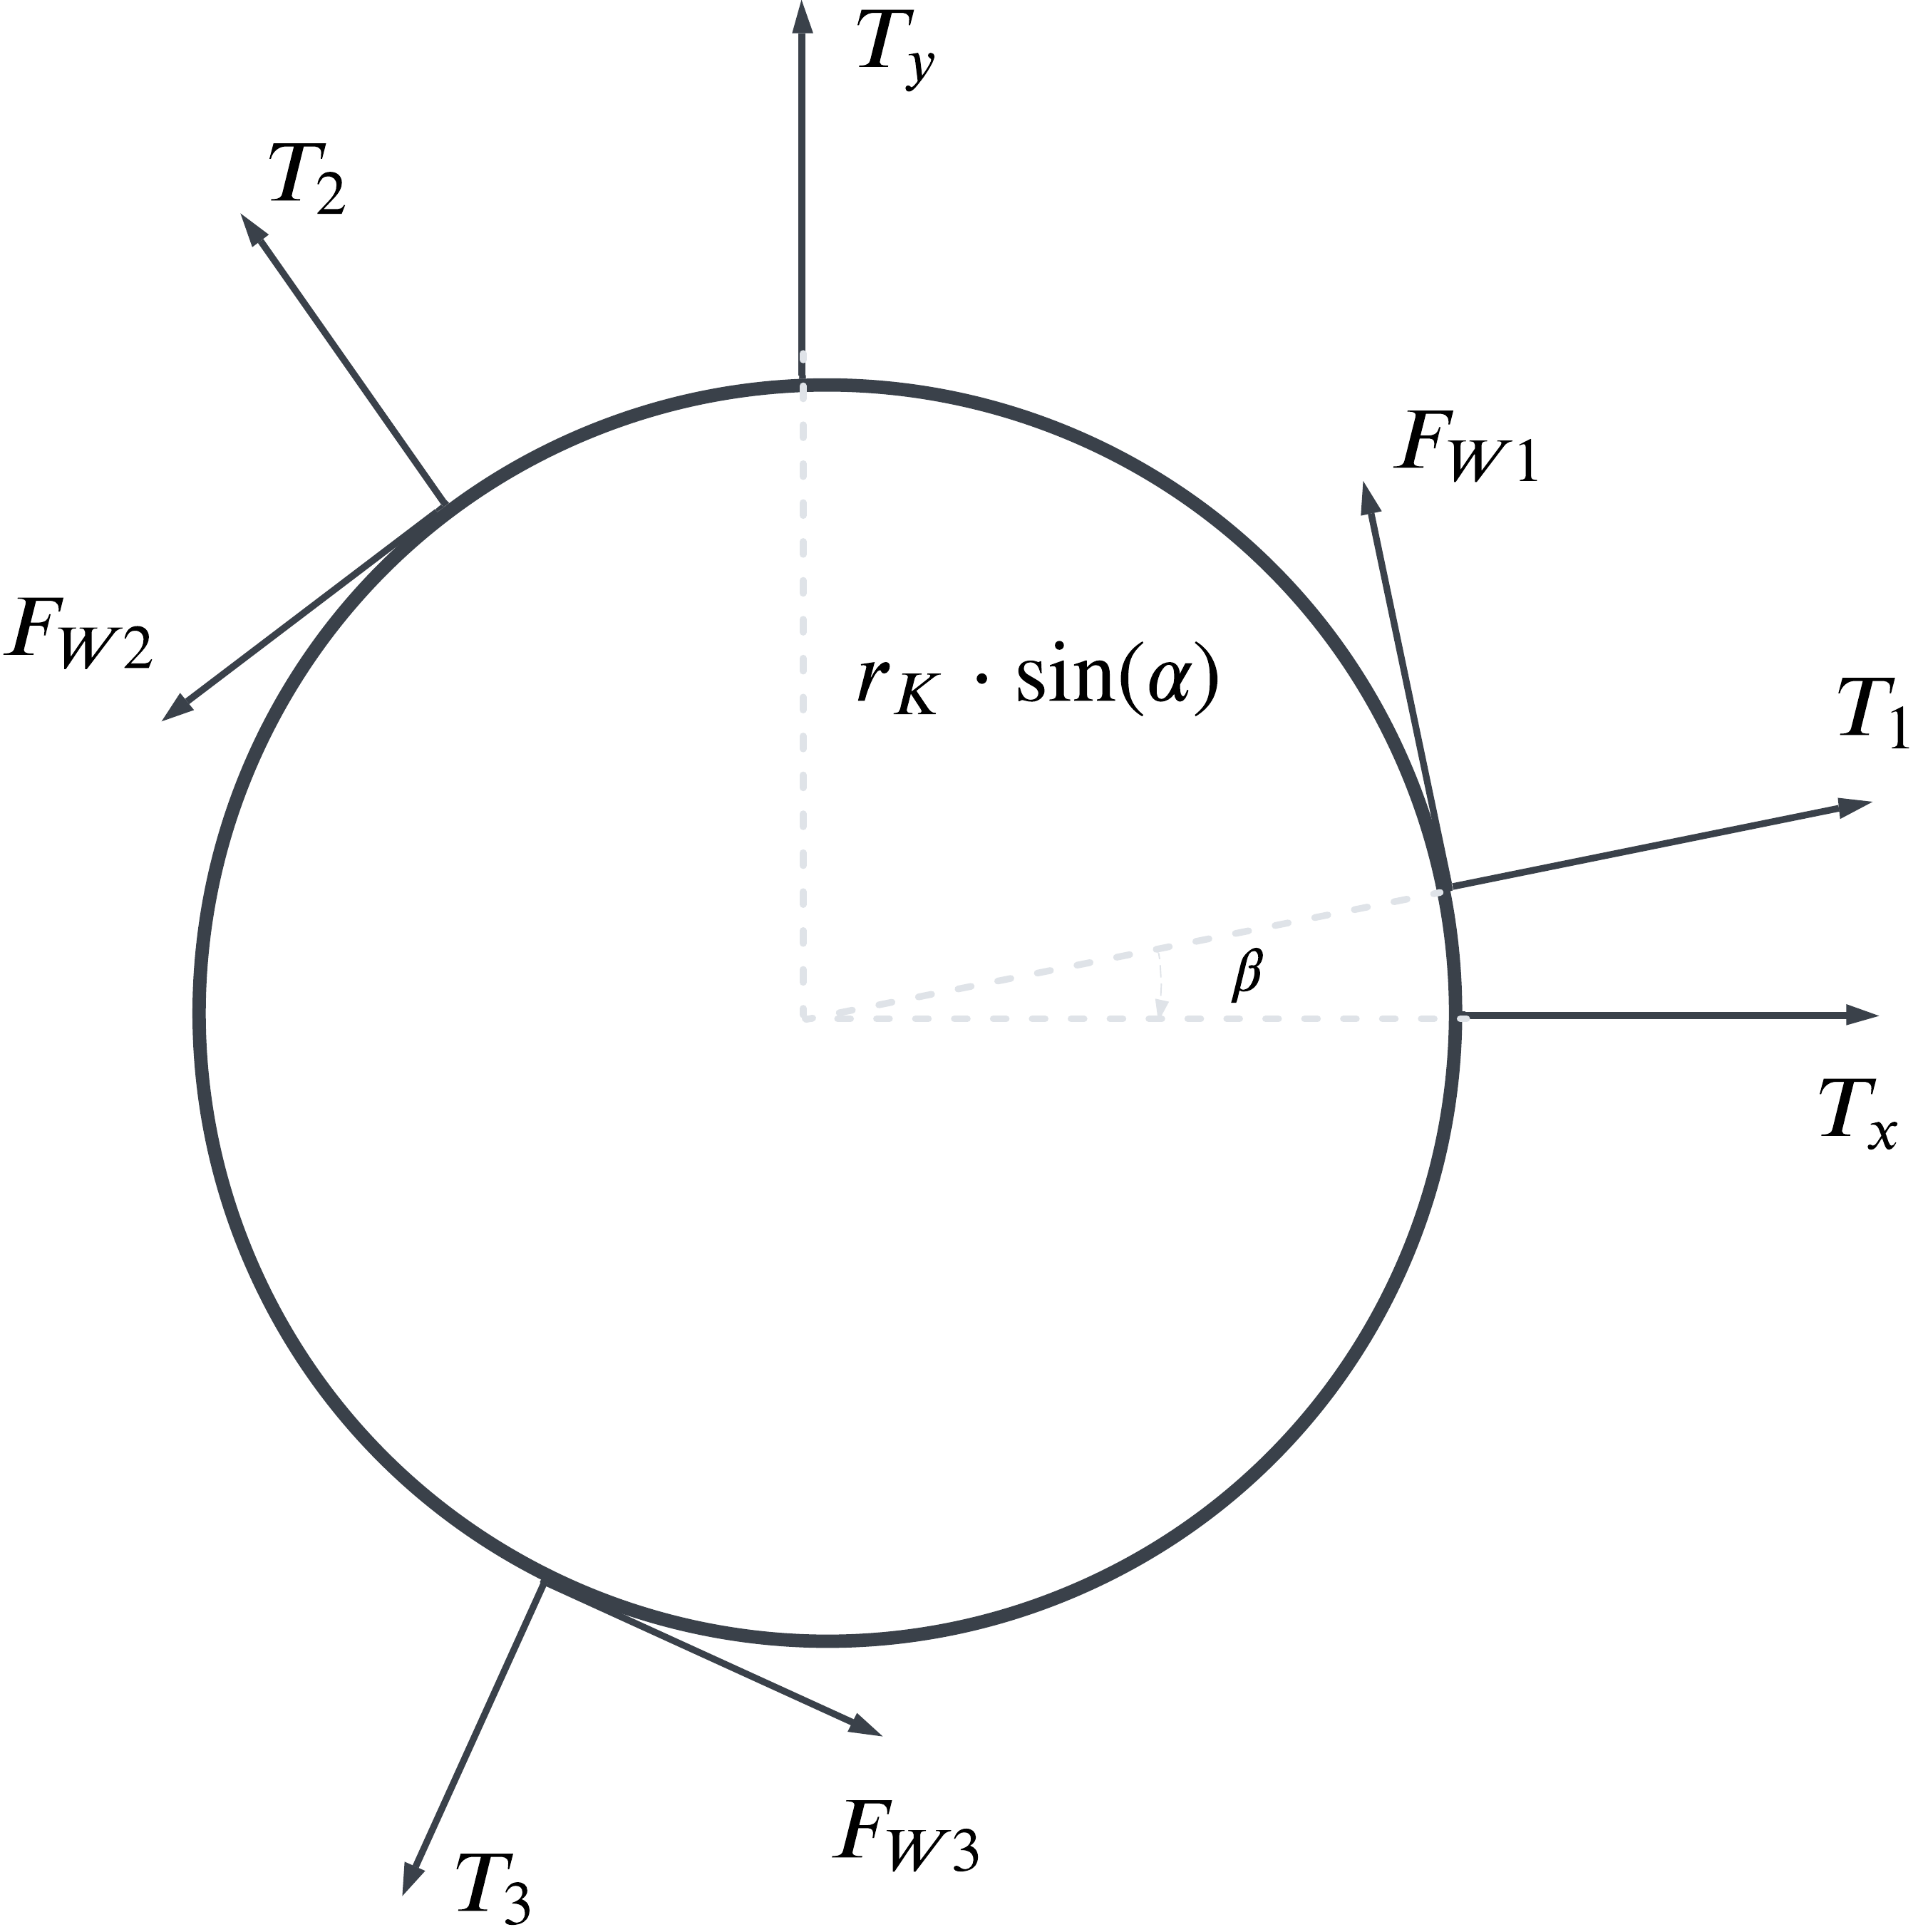
\includegraphics[width=\linewidth]{Metodologia/Figuras/torque_up.png}
        \caption{Modelo real visto de cima}
        \label{fig:torques_cima}
    \end{subfigure}
\end{figure}

Usando esses modelos, obteve-se as forças tangentes provocadas pelo torque dos motores:

\begin{equation}
    \begin{aligned}
    F_{W,1} &= \frac{T_1}{r_W} 
    \begin{bmatrix}
    -\sin \beta \\
    \cos \beta \\
    0
    \end{bmatrix}, \\
    F_{W,2} &= \frac{T_2}{r_W} 
    \begin{bmatrix}
    -\sin \left( \beta + \frac{2}{3}\pi \right) \\
    \cos \left( \beta + \frac{2}{3}\pi \right) \\
    0
    \end{bmatrix}, \\
    F_{W,3} &= \frac{T_3}{r_W} 
    \begin{bmatrix}
    -\sin \left( \beta - \frac{2}{3}\pi \right) \\
    \cos \left( \beta - \frac{2}{3}\pi \right) \\
    0
    \end{bmatrix}.
    \end{aligned}
\end{equation}

Os braços de alavanca também foram obtidos:

\begin{equation}
    \begin{aligned}
        r_{KW,1} &= r_K \cdot 
        \begin{bmatrix}
        \cos \beta \sin \alpha \\
        \sin \beta \sin \alpha \\
        \cos \alpha
        \end{bmatrix}, \\
        r_{KW,2} &= r_K \cdot 
        \begin{bmatrix}
        \cos \left( \beta + \frac{2}{3}\pi \right) \sin \alpha \\
        \sin \left( \beta + \frac{2}{3}\pi \right) \sin \alpha \\
        \cos \alpha
        \end{bmatrix}, \\
        r_{KW,3} &= r_K \cdot 
        \begin{bmatrix}
        \cos \left( \beta - \frac{2}{3}\pi \right) \sin \alpha \\
        \sin \left( \beta - \frac{2}{3}\pi \right) \sin \alpha \\
        \cos \alpha
        \end{bmatrix}.
    \end{aligned}
\end{equation}

Ainda, obteve-se as forças tangentes nos modelos planares e seus braços de alavanca:

\begin{equation}
    \begin{aligned}
    F_{W,x} &= \frac{T_x}{r_W} \cdot 
    \begin{bmatrix}
    0 \\ 
    1 \\ 
    0
    \end{bmatrix}, \\
    F_{W,y} &= \frac{T_y}{r_W} \cdot 
    \begin{bmatrix}
    1 \\ 
    0 \\ 
    0
    \end{bmatrix}, \\
    F_{W,z} &= \frac{T_z}{r_W} \cdot 
    \begin{bmatrix}
    -\sin \beta \\ 
    \cos \beta \\ 
    0
    \end{bmatrix}, \\
    r_{KW,x} = r_{KW,y} &= r_K \cdot 
    \begin{bmatrix}
    0 \\ 
    0 \\ 
    1
    \end{bmatrix}, \\
    r_{KW,z} &= r_K \cdot 
    \begin{bmatrix}
    \cos \beta \cdot \sin \alpha \\ 
    \sin \beta \cdot \sin \alpha \\ 
    0
    \end{bmatrix}.
    \end{aligned}
\end{equation}

Portanto, os torques na bola no modelo real e nos modelos planares são:

\begin{equation}
    \begin{aligned}
    T_{KW,i} &= r_{KW,i} \times F_{W,i} \quad \text{para } i = 1, 2, 3, \\
    T_{KW,j} &= r_{KW,j} \times F_{W,j} \quad \text{para } j = x, y, z.
    \end{aligned}
\end{equation}

Como o torque total deve ser conservado, usou-se a equação

\begin{equation}
    T_{KW,1} + T_{KW,2} + T_{KW,3} = T_{KW,x} + T_{KW,y} + T_{KW,z}
\end{equation}

para calcular o torque dos motores reais e o torque dos motores virtuais:

\begin{align*}
T_1 &= \frac{1}{3} \left( T_z + \frac{2}{\cos \alpha} \cdot \left( T_x \cdot \cos \beta - T_y \cdot \sin \beta \right) \right) \\
T_2 &= \frac{1}{3} \left( T_z + \frac{1}{\cos \alpha} \cdot \left( \sin \beta \cdot \left( -\sqrt{3} T_x + T_y \right) - \cos \beta \cdot \left( T_x + \sqrt{3} T_y \right) \right) \right) \\
T_3 &= \frac{1}{3} \left( T_z + \frac{1}{\cos \alpha} \cdot \left( \sin \beta \cdot \left( \sqrt{3} T_x + T_y \right) + \cos \beta \cdot \left( -T_x + \sqrt{3} T_y \right) \right) \right)
\end{align*}

\begin{align*}
T_x &= \cos \alpha \cdot \left( T_1 \cdot \cos \beta - T_2 \cdot \sin \left( \beta + \frac{\pi}{6} \right) + T_3 \cdot \sin \left( \beta - \frac{\pi}{6} \right) \right) \\
T_y &= \cos \alpha \cdot \left( -T_1 \cdot \sin \beta - T_2 \cdot \cos \left( \beta + \frac{\pi}{6} \right) + T_3 \cdot \cos \left( \beta - \frac{\pi}{6} \right) \right) \\
T_z &= T_1 + T_2 + T_3
\end{align*}

\subsection{Cálculos de inércia}

A inércia da bola foi aproximada por uma esfera oca, 

\begin{equation*}
    \Theta_K = \frac{2}{3} \cdot m_K \cdot r_K^2,
\end{equation*}

enquanto o corpo foi aproximado por um cilindro:

\begin{equation*}
    \Theta_A = \frac{1}{4} \cdot m_A \cdot r_A^2 + \frac{1}{2} \cdot m_A \cdot h^2 + m_A \cdot l^2,
\end{equation*}

\begin{equation*}
    \Theta_{A,xy} = \frac{1}{2} \cdot (m_A + m_W) \cdot r_A^2.
\end{equation*}

Dado o momento de inércia do motor, $\Theta_M$, e o momento de inércia da roda omnidirecional,

\begin{equation}
    \Theta_{OW} = \frac{1}{2} \cdot m_{OW} \cdot r_W^2
\end{equation},

onde $m_{OW}$ é a massa da roda omnidirecional.

Ainda, há o momento de inércia das rodas virtuais, que foi obtido comparando a energia rotacional em torno de um eixo no sistema virtual com a energia rotacional em torno do mesmo eixo no sistema real.

As velocidades angulares da rodas na direção $y$ são:

\begin{align*}
\omega_{OW,1} &= \omega_{W,x} \cos \alpha \\
\omega_{OW,2/3} &= -\frac{1}{2} \omega_{W,x} \cos \alpha
\end{align*}

Enquanto na direção $x$ são:

\begin{align*}
\omega_{OW,1} &= 0 \\
\omega_{OW,2} &= -\frac{\sqrt{3}}{2} \omega_{W,y} \cos \alpha \\
\omega_{OW,3} &= \frac{\sqrt{3}}{2} \omega_{W,y} \cos \alpha
\end{align*}

Por fim, na direção z:

\begin{equation*}
    \omega_{OW,1/2/3} = \omega_{W,z} \sin \alpha
\end{equation*}.

Fazendo o quilibrio energético na direção y,
\begin{align*}
\frac{1}{2} \Theta_{W,x} \dot{\psi}_x^2 &= \frac{1}{2} \Theta_{OW} (\dot{\psi}_x \cos \alpha)^2 + \frac{1}{2} \Theta_M (\dot{\psi}_x \cos \alpha)^2 \\
&\quad + \frac{1}{2} \cdot 2 \left( \Theta_{OW} \left(-\frac{1}{2} \dot{\psi}_x \cos \alpha \right)^2 + \Theta_M \left(-\frac{1}{2} \cdot \dot{\psi}_x \cos \alpha \right)^2 \right) \\
\Theta_{W,x} &= \cos^2(\alpha) \left( \Theta_{OW} + \Theta_M + \frac{1}{2} \left( \Theta_{OW} + \Theta_M \right) \right) \\
&= \frac{3}{2} \cos^2(\alpha) \left( \Theta_{OW} + \Theta_M \right)
\end{align*},

e na direção x,
\begin{align*}
\frac{1}{2} \Theta_{W,y} \dot{\psi}_y^2 &= \frac{1}{2} \cdot 2 \left( \Theta_{OW} \left(\frac{\sqrt{3}}{2} \dot{\psi}_y \cos \alpha \right)^2 + \Theta_M \left(-\frac{\sqrt{3}}{2} \cdot \dot{\psi}_x \cos \alpha \right)^2 \right) \\
\Theta_{W,y} &= \frac{3}{2} \cos^2(\alpha) (\Theta_{OW} + \Theta_M),
\end{align*}

usando a notação.

\begin{align*}
\dot{\psi}_x &= \omega_{W,x} \\
\dot{\psi}_y &= \omega_{W,y} \\
\dot{\psi}_1 &= \omega_{OW,1} \\
\dot{\psi}_2 &= \omega_{OW,2} \\
\dot{\psi}_3 &= \omega_{OW,3}.
\end{align*}

tem-se, portanto,

\begin{align*}
\Theta_{W} = \Theta_{W,x} = \Theta_{W,y} = \frac{3}{2} \cos^2(\alpha) (\Theta_{OW} + \Theta_M).
\end{align*}

Seguindo-se o mesmo procedimento para o plano $x$-$y$ obteve-se:

\begin{align*}
    \Theta_{W,xy} = 3 \cdot (\Theta_{OW} + i^2 \cdot \Theta_M).
\end{align*}


\section{Projeto de controladores}
\label{sec:projetocontroladores}

\clearpage
\chapter{Resultados}

Para a execução do projeto, algumas etapas de desenvolvimento tiveram de ser seguidas: familiarização com o sistema, estudo dos módulos envolvidos, leitura dos requisitos, elaboração de documento descrevendo todo o processo de implementação e relacionamento com os diversos módulos, implementação e testes.


\section{Atividades do Projeto}
\label{metodo3}

\section {Requisitos do Sistema}
\label{req}


\section{Desenvolvimeto e Implementação}

A Tabela \ref{tab:tabela} apresenta as atividades executadas.

\begin{table}
\centering
%Note os alinhamentos diferentes em cada coluna
\begin{tabular}{|c|r|l|}\hline
		Atividade 1 & aa  & ab  \\ 
					 & a & b \\ \hline
		Ativ. 2  & aa & ab \\			
					 &  a & b \\ \hline
		\end{tabular}
	\caption{Exemplo de tabela - Coloque toda informação sobre a tabela aqui}
	\label{tab:tabela}
\end{table}

\section{Testes}

\section{Análise dos Resultados}

Apresente os resultados sem adulterações e faça análises objetivas. Pense na melhor maneira de apresentar os resultados graficamente. Se os gráficos são difíceis de interpretar, talvez tabelas sejam uma forma melhor de apresentar resultados. Não apresente dados (gráficos e tabelas) se não há uma conclusão interessante a ser tirada. Lembre-se de ser conciso.

\emph{Não se esqueça das unidades!} Pense que \emph{a priori} todo número deve ter uma unidade. Não escreva as unidades em itálico (no ambiente matemático) e tome cuidado para diferenciar maiúsculas e minúsculas. Um exemplo é escrever $22$ [kN] e não $22 KN$ (Kelvin vezes Newton!).

Ao apresentar resultados experimentais, tome o cuidado para também apresentar o cálculo das incertezas sempre que forem significativas. Ao fazer conclusões, sempre considere se o tamanho da sua amostra é grande o suficiente do ponto de vista estatístico. Lembre que a média empírica $\hat{\mu}_X$ de $N$ observações independentes da variável $X_i$ possui variância
\[
\hat{\sigma}_{\mu}^2 = \frac{1}{N(N-1)} \sum_{i=1}^N (X_i-\hat{\mu}_X)^2
\enspace,
\]
onde se assume que as variáveis $X_i$ possuem uma mesma ditribuição e que essa distribuição possui segundo momento finito.


\section{Resumo do Capítulo}
\label{sec:resumoo4}
Tente não terminar de forma abrupta. Se for escrever algo aqui, não seja genérico!

\section{Formato, expressões matemáticas e o \LaTeX}

\subsection{O \LaTeX}

O {\LaTeX}  é o método preferencial de preparação de documentos para textos técnicos nas ciências exatas. O {\LaTeX} permite não só lidar com equações de uma forma mais prática que em editores de texto, mas também facilita a formatação de documentos e tem um desempenho marcadamente superior a editores de texto na preparação de documentos longos como monografias. 

Documentos em {\LaTeX} são escritos em um ou mais arquivos de texto com extensão .tex. Após a escrita, o .tex é \emph{compilado} para gerar arquivos nos formatos .pdf, .dvi ou .ps. Hoje há duas distribuições padrão para o \LaTeX. Sistemas Windows usam o {Mik\TeX} e sistemas Unix usam o \TeX Live. Além das distribuições, muitos usuários utilizam \emph{front-ends} que facilitam a edição do texto, a compilação e a instalação de pacotes. 

Os pacotes necessários para compilar o presente documento devem ser encontrados numa instalação completa dessas distribuições. Se tiver dificuldades com os pacotes, você pode instalá-los manualmente ou tentar alterar o código para usar versões antigas dos mesmos.

A compilação pode ser feita pelos comandos \textsf{latex} ou \textsf{pdflatex}, invocados pela linha de comando ou pelo \emph{front-end}. Note que será necessário empregar o comando \textbf{mais de uma vez} para que as referências cruzadas saiam corretas.

Como discutido na Seção \ref{sec:revisão}, uma ferramenta útil para gerenciar as citações em {\LaTeX} é o Bib\TeX. Para gerar uma lista bibliográfica a partir do arquivo .bib, este arquivo deve ser indicado no arquivo .tex. Em seguida devem-se executar os comandos \textsf{pdflatex}, \textsf{bibtex} e \textsf{pdflatex} novamente sempre usando o .tex como argumento. Note que os comandos são executados nesta ordem e de forma repetida para que as referências cruzadas sejam geradas corretamente.

Nesta seção você deve encontrar exemplos dos comandos mais usados em \LaTeX. Outros exemplos e manuais podem ser encontrados na internet com facilidade.

\subsection{Expressões Matemáticas}

Ao escrever expressões matemáticas, defina todas as variáveis antes de usá-las ou imediatamente depois da expressão. Deixar de fazê-lo torna seu texto \textbf{ilegível}. Segue um exemplo.

Seja o par $(a_1,a_2)\in \mathbb{R}^2$. Para $s\in\mathbb{C}$, definimos a função $f(s)$ como
\[%cria equações sem numeração
f(s)\triangleq \frac{a_1 s+a_2}{s^2+2\zeta\omega_n s+\omega_n^2}
\enspace,
\]
onde os escalares $\zeta,\omega_n>0$ são constantes.

Note que não foi necessário atribuir valores às variáveis neste momento. Repare também como devemos \textbf{usar pontuação} (vírgula) nas equações, tratando-as como parte da frase. Usamos o símbolo $\triangleq$ ou $:=$ para deixar explícito que se trata de uma definição. Ser claro nesse aspecto facilita o entendimento do leitor.

A equação acima não foi numerada porque não será citada no texto. Vejamos um exemplo com numeração.

A função $f(\cdot)$ possui um zero em $-a_2/a_1$ (ou $-\frac{a_2}{a_1}$) e, para $\zeta<1$, possui polos complexos $p_{1,2}$ dados por
\begin{equation}
\label{eq:polos}
p_{1,2}=\omega_n \left(-\zeta\pm j\sqrt{1-\zeta^2}\right)
\enspace.
\end{equation}
Agora podemos citar os polos dados pela Equação (\ref{eq:polos}) (aqui adotamos a convenção de citar sempre com o número entre parênteses precedido da palavra Equação). Note como usamos um comando especial na Equação \ref{eq:polos} para garantir o ajuste automático do tamanho dos parênteses.

Vejamos agora como criar equações alinhadas. Considere o sistema dinâmico dado pelas equações diferenciais:

\begin{align}
\dot{x}_1 & = \cos(x_2)\cdot\ln(1/x_1)+\tan(u) \label{eq:x1dot} \\
\dot{x}_2 & = e^{-x_1-x_2} \nonumber \\
& y  = \min\{x_1,x_2\}  \label{eq:saida}
\enspace,
\end{align}
onde $x(t)=[x_1(t) ~ x_2(t)]'$, $t>0$, é a variável de estado do sistema, $u(t)$ é o sinal de entrada e $y(t)$ é o sinal de saída do sistema. Note no .tex que o caracter de tabulação \textsf{\&} foi usado para indicar o ponto de alinhamento horizontal das equações. Além disso, para ilustrar o uso do \LaTeX, retiramos a numeração da segunda equação e citamos as equações separadamente.

Nas Equações (\ref{eq:x1dot}) e (\ref{eq:saida}), aparecem operadores como $\min$, $\ln$, $\cos$ e $\tan$. A convenção aqui é que \textbf{variáveis devem ser escritas em itálico e operadores não}. Por essa razão todas as expressões matemáticas devem ser escritas no ambiente matemático (entre cifrão) mesmo quando for possível usar texto comum. Isso garante a consistência das fontes utilizadas (nem sempre a fonte do ambiente matemático é a mesma fonte do texto). 

Para escrever matrizes, podemos fazer por exemplo:
\[
\sum_{n=0}^{\infty}z^{-n}\left[\begin{array}{cc}
\lambda & 1 \\
0 & \lambda
\end{array}\right]^n=
\left[\begin{array}{cc}
\frac{z}{z-\lambda} & \frac{z}{(z-\lambda)^2} \\
0 & \frac{z}{z-\lambda}
\end{array}\right]
,~\forall \lambda<|z|
\enspace.
\]

Para escrever uma expressão com múltiplos casos, podemos fazer, para um inteiro $N$ positivo,
\[
g[n]=
\left\{
\begin{array}{ll}
0,& \mbox{se }~ n\leq 0 \\
n,& \mbox{se }~ n=1,2,\ldots,N-1 \\
N,& \mbox{se }~ n\mod N = 0 \\
0,& \mbox{caso contrário}\enspace.
\end{array}
\right.
\]

\textbf{Nunca reaproveite símbolos} matemáticos, isto é, nunca use o mesmo símbolo para designar variáveis diferentes.

Para um exemplo com múltiplas linhas de expressão matemática: tem-se que, para $a\neq 0$,

\begin{equation}
\begin{split}
ax^2+bx+c &= 0 \\
& \Rightarrow a(x^2+bx/a+c/a) =0 \Rightarrow a((x+b/(2a))^2+c/a-b^2/(4a^2))=0  \\
& \Rightarrow (x+b/(2a))^2=(b^2-4ac)/(4a^2) \\
& \Rightarrow (x+b/(2a))=\pm\sqrt{b^2-4ac}/(2a) \\
& \Rightarrow x=\frac{-b\pm\sqrt{b^2-4ac}}{2a}
\enspace.
\end{split}
\end{equation}

Note a argumentação lógica aqui. Não estamos dizendo que o valor de $x$ é dado pela última linha. Estamos dizendo que a hipótese da primeira linha juntamente com a hipótese $a\neq 0$ implicam os referidos valores de $x$. \textbf{Um erro comum dos alunos ao escrever é não distinguir a veracidade das implicações com a veracidade das hipóteses}.

\clearpage
\chapter{Conclusões}

Novamente, este será um dos trechos que o leitor experiente lerá antes de decidir se vale a pena ler o texto integral. Seja convincente.

\section{Considerações Finais}

Reitere o que de mais importante foi feito, qual era o objetivo inicial e qual o resultado obtido. Se houve requisitos ou especificações de projeto, discuta se foram atingidos. Se os resultados não foram conclusivos ou contrariam o que se esperava, seja honesto e diga-o explicitamente. Busque explicar os insucessos com argumentos sólidos e plausíveis. 

\section{Propostas de Continuidade}

Se houve questões ainda não respondidas ou resultados insatisfatórios, aponte direções de continuação.

\clearpage


\addcontentsline{toc}{chapter}{Referências Bibliográficas}
\renewcommand{\bibname}{Referências Bibliográficas}

%\bibliographystyle{abntex2-alf} %para norma ABNT no sistema autor-data
\bibliographystyle{abntex2-num}
\begin{small}
\bibliography{ListadeReferencias}%,library}
%% Monografia para Projeto de Fim de Curso - Exemplo no LaTeX
%-----------------------------------------------------------


%---------------Inicialização de pacotes--------------------

\documentclass[12pt,a4paper,notitlepage,twoside]{book}


\usepackage{graphicx}
\usepackage[utf8]{inputenc}
%\usepackage[latin1]{inputenc} %%pode ser necessário trocar a codificação em sistemas Windows
\usepackage[brazil]{babel}		%%pode ser necessário trocar o pacote de línguas em algumas distribuições LateX
%\usepackage[portuguese]{babel}
\usepackage[T1]{fontenc}
\usepackage{amsmath,amssymb}
\usepackage{amsthm,amsfonts}
\usepackage{color}
\usepackage[colorlinks]{hyperref}
\usepackage{abntex2abrev}
%\usepackage[alf]{abntex2cite} %se você quiser seguir as normas ABNT no sistema autor-data
%\usepackage[num]{abntex2cite} %se você quiser seguir as normas ABNT no sistema numérico
\usepackage{setspace}
\usepackage[toc,page]{appendix}

%Definindo fonte Times (Use os pacotes obsoletos se não conseguir instalar os atualizados)
%\usepackage{times}     %Pacote de fontes obsoleto, apenas texto
%usepackage{mathptmx}  %Pacote de fontes obsoleto, texto e símbolos matemáticos
%\usepackage{newtxtext,newtxmath}  %Pacotes de fontes mais recentes

\usepackage[a4paper,top=30mm,bottom=30mm,inner=30mm,outer=25mm,headheight=7mm,headsep=6mm,footskip=7mm]{geometry}
\usepackage{enumerate}
\usepackage{tabularx}
\usepackage{array} % Necessário para o alinhamento vertical
\usepackage{makecell} % Para controle uniforme da altura das linhas
\usepackage{float}    % Para fixar a tabela no local desejado
\usepackage{subcaption} % Alinhar imagens lado a lado
\usepackage{graphicx} % Reduzir tamanho da fonte de uma equação

\makeindex

%\singlespacing   %%espaçamento simples
%\onehalfspacing
%\setstretch{1.03} %%um pouco melhor que espaçamento simples
\linespread{1.25} %corresponde ao espaçamento 1.5 do MS Word

%---------------Início do documento-------------------------

\begin{document}

\setlength{\extrarowheight}{4pt} % Define uma altura extra para as linhas

\begin{titlepage}
\begin{center}
{\large Universidade Federal de Minas Gerais\\
Escola de Engenharia \\
Curso de Graduação em Engenharia de Controle e Automação\\}

\vspace{6cm}
{\bf\Large Construção, modelagem, projeto de controlador e implementação em hardware para um pêndulo invertido sobre uma esfera\vspace{0.2cm}}
\vspace{4cm}

%\hspace{0.3\textwidth} \parbox{0.65\textwidth}
{\large Samuel Soares do Patrocínio}
\vspace{2cm}  
   
\vspace{2cm}          
%\hspace{0.3\textwidth} 
{\large Orientador: Prof. Fernando de Oliveira Souza}\\
%{\large Supervisor: Eng. Cicrano}

\vfill
%\hspace{0.3\textwidth} 
{\large Belo Horizonte, Novembro de 2024 }
\end{center}

\end{titlepage}

\newpage
\clearpage
\thispagestyle{empty}


\begin{titlepage}

\centering
\textbf{Monografia}\\
\vspace{2cm}
\centering
\textbf{Construção, modelagem, projeto de controlador e implementação em hardware para um pêndulo invertido sobre uma esfera}\\
\vspace{5cm} 

\parbox{1.0\textwidth} 
{\large 
Monografia submetida à banca examinadora
designada pelo Colegiado Didático do Curso de
Graduação em Engenharia de Controle e
Automação da Universidade Federal de Minas
Gerais, como parte dos requisitos para aprovação na
atividade Projeto Final de Curso II.}

\vspace{7cm} 
\centering
Belo Horizonte, Julho de 2014

\end{titlepage}


\pagenumbering{roman}
\addcontentsline{toc}{chapter}{Resumo}

\begin{center}
\huge{{\bf Resumo}}
\vspace{2cm}
\end{center}

No Resumo, em uma única página, em no máximo dois parágrafos, você explicita os seguintes itens: objetivos do projeto e descrição sucinta do local onde ele foi desenvolvido; metodologia utilizada; e resultados alcançados. Leitores experientes decidem se prosseguirão para a leitura do texto completo após lerem o resumo, a conclusão e a introdução. Por isso nestes lugares você deve colocar um esforço maior de convencimento. Além disso, a linguagem utilizada deve ser acessível a leitores com pouca familiaridade com a área, limitando-se o uso de jargões.
 
\begin{sloppypar}
Este novo parágrafo serve para mostrar que ao pular uma ou mais linhas no texto do arquivo .tex, o \TeX\ entende que você está iniciando outro parágrafo. O comando \textsf{sloppypar} força o texto a não ultrapassar as margens. Só deve ser usado se este problema ocorrer.
\end{sloppypar}

 
\clearpage
\thispagestyle{empty}
\cleardoublepage


\addcontentsline{toc}{chapter}{Abstract}

\begin{center}
\huge{{\bf Abstract}}
\vspace{2cm}
\end{center}

Write a version of your ``resumo'' in English. Beware of literal translations and double check the translation of technical terms.
 

 
\clearpage
\thispagestyle{empty}
\cleardoublepage


\addcontentsline{toc}{chapter}{Agradecimentos}

\begin{center}
\huge{{\bf Agradecimentos}}
\vspace{4cm}
\end{center}

Aqui vai o texto dos agradecimentos.
 
\clearpage
\thispagestyle{empty}
\cleardoublepage
\tableofcontents
%\markboth{Conteúdo}{Conteúdo}

\clearpage
%\thispagestyle{empty}
%\cleardoublepage

% Normalmente, este arquivo só contém isto.
\listoffigures
\addcontentsline{toc}{chapter}{Lista de Figuras}
%\markboth{Lista de Figuras}{Lista de Figuras}

\clearpage
%\thispagestyle{empty}
%\cleardoublepage

% Normalmente, este arquivo só contém isto.
\listoftables
\addcontentsline{toc}{chapter}{Lista de Tabelas}
%\markboth{Lista de Tabelas}{Lista de Tabelas}

\clearpage
%\thispagestyle{empty}
%\cleardoublepage

% Normalmente, este arquivo só contém isto.

\pagenumbering{arabic}
\setcounter{page}{1}
\chapter{Introdução}
\label{chap:intro} %este label será usado para referenciar este capítulo

%As primeiras frases têm a missão de prender a atenção do leitor e por isso são as mais importantes do texto. Diga o quanto antes o que você fez e quais são os resultados alcançados. Ao terminar de ler a introdução o leitor tomará uma nova decisão de se vale a pena ou não continuar lendo o texto. Capte a atenção do leitor bem aqui.

%A comunicação escrita é considerada umas das cinco habilidades mais importantes por profissionais de engenharia e um engenheiro passa em média mais de $25$\% do seu tempo escrevendo \cite{eggert2002response,spretnak1982survey}. Uma quantidade similar de tempo é gasta na escrita de correspondência e de relatórios técnicos \cite{cunningham2012perceptions}. Dessa forma, encare a escrita do seu projeto como um treinamento nessa importante habilidade.

%Neste texto você encontrará não apenas uma estrutura para escrever seu trabalho em \LaTeX, mas também um pequeno manual de boas práticas na escrita técnica. Leia com atenção e coloque as sugestões em prática à medida que preenche o texto com o conteúdo do seu próprio projeto. Também será apresentado um número de vícios de escrita comumente encontrados nas monografias de alunos. 

%A seguir está a estrutura de organização sugerida pelo colegiado do curso. Note que ela não é necessariamente a melhor para contar a história do seu projeto. Você pode por exemplo preferir usar títulos mais pertinentes ao seu contexto. Contudo, o seu texto deve conter cada um dos pontos a seguir.

\section{Motivação e Justificativa}
\label{sec:motivacao}

O avanço contínuo na área de controle e automação exige que os futuros engenheiros dominem técnicas práticas e teóricas para solucionar problemas reais de engenharia. No contexto do curso de Engenharia de Controle e Automação, é essencial que os alunos tenham acesso a plataformas de aprendizagem que unam teoria e prática de maneira dinâmica e interativa. Nesse cenário, o desenvolvimento de sistemas experimentais versáteis e acessíveis é uma abordagem eficiente para consolidar o aprendizado e despertar o interesse por sistemas de controle complexos.

O projeto proposto consiste na construção de um robô que se equilibra sobre uma esfera, uma aplicação concreta do conceito de pêndulo invertido. Esse sistema é amplamente utilizado no ensino de técnicas de controle devido à sua natureza desafiadora e suas características dinâmicas, que exigem uma compreensão aprofundada de modelagem, análise e implementação de controladores.

A utilização de modelagem 3D e impressão em impressoras 3D para a construção do robô garante um custo reduzido, acessível tanto para o laboratório quanto para alunos interessados em replicar o projeto. Essa abordagem também assegura que eventuais danos à planta possam ser facilmente reparados, incentivando o uso contínuo e livre do sistema pelos discentes. Dessa forma, o projeto atende a dois objetivos principais: a oferta de um sistema dinâmico e interessante para o estudo de controle e a promoção de um ambiente de aprendizagem prático e sustentável.

%Argumente sobre a importância do projeto desenvolvido usando uma visão de alto nível, sem entrar em detalhes. Contextualize seu projeto dentro do local de execução ou da literatura e explique como ele é necessário ou inovador. É possível fazer uma breve revisão bibliográfica, confrontando seu trabalho com outras referências bibliográficas para mostrar a sua contribuição. No quesito contribuição, é muito importante deixar claro o tempo todo que partes do projetos foram executadas por outros e que partes foram executadas por você. Caso contrário, corre-se o risco de inadvertidademente tomar crédito pelo trabalho de outrem, o que pode ter implicações legais. 

\section{Objetivos do Projeto}
\label{sec:objetivos}

Tendo em vista o exposto acima, este projeto tem por objetivos:

\begin{enumerate}[a)]
\item  Projetar e construir um robô do tipo pêndulo invertido que se equilibra sobre uma esfera, utilizando conceitos aprendidos ao longo do curso de Engenharia de Controle e Automação;
\item Tornar a construção viável e replicável por meio da utilização de impressão 3D, proporcionando durabilidade e acessibilidade; 
\item Implementar e validar técnicas de controle avançadas para garantir a estabilidade do sistema e seu funcionamento eficiente.

Esses objetivos foram estabelecidos com a finalidade de integrar o conhecimento teórico adquirido ao longo do curso com aplicações práticas relevantes, contribuindo para a formação de engenheiros mais preparados para lidar com desafios reais.
\end{enumerate}

%O conteúdo desta seção pode se sobrepor um pouco com o da seção anterior, podendo ela ser um sumário dos pontos expostos anteriormente. A escolha do título da seção talvez seja mais apropriada para a fase de proposta do projeto. Afinal, nesta fase se conhecem os objetivos e não os resultados. Por outro lado, fará pouco sentido discutir objetivos quando o projeto está finalizado, especialmente se tais objetivos não foram alcançados. 


\section{Local de Realização}
\label{sec:empresa}

O desenvolvimento do projeto será realizado no Laboratório de Controle da Escola de Engenharia da Universidade Federal de Minas Gerais (UFMG). A impressão das peças será viabilizada por meio de uma impressora 3D disponibilizada pelo professor Fernando de Oliveira Souza, que também supervisionará as etapas práticas e fornecerá o suporte técnico necessário.


\section{Estrutura da Monografia}
\label{sec:organizacao}

Esta monografia está organizada em quatro capítulos, além desta introdução. O Capítulo 1 apresenta uma visão geral do projeto, incluindo sua motivação, objetivos e local de execução. O Capítulo 2 explora os princípios fundamentais relacionados ao pêndulo invertido, detalhando conceitos essenciais para o entendimento do sistema e do controle aplicado. O Capítulo 3 descreve a metodologia adotada no projeto, abrangendo as etapas de modelagem 3D, construção da planta física, modelagem matemática e projeto dos controladores. Por fim, o Capítulo 4 apresenta as conclusões obtidas, as contribuições do projeto e sugestões para trabalhos futuros, além de relatar os principais desafios enfrentados.


\clearpage
\chapter[Descrição do Processo]{Descrição do Problema/Processo ou O Processo de Fazer Alguma Coisa}
\label{chap:descricaoproblema}
%Note que, como nome do capítulo é muito longo, fornecemos um nome abreviado uso no cabeçalho

Se desejar, uma visão geral do capítulo pode ser colocada antes da primeira seção. Este é o capítulo de descrição do processo e formulação do problema. Tendo em vista que se trata de uma monografia de engenharia de controle e automação, em muitos casos será fundamental a apresentação dos sensores e atuadores do processo.


\section{Processo de Fazer Alguma Coisa}
\label{sec:hist}

Cada seção inicia pela descrição do seu conteúdo e pode terminar com um parágrafo de conexão com a seção seguinte. 

Antes de formular o problema, \textbf{não se esqueça de fazer todas as definições necessárias}. Também devem-se detalhar os aspectos complementares da abordagem: se estamos estudando um aspeto particular do problema, se a resposta encontrada é universal ou dependente de simplificações e hipóteses prévias.


\section{Instrumentação do Processo}
\label{sec:instrumentação}

Descreva a aparelhagem e o equipamento utilizados bem como a ligação entre os diversos componentes. Nesta seção e, ao longo de todo o texto, você deve dar detalhes suficientes para que qualquer pessoa consiga reproduzir seus experimentos.

Contudo, \textbf{não disperse o leitor com detalhes irrelevantes} ou aspectos
demasiado técnicos ou formais. Reserve tais detalhes para um
apêndice.

Como uma imagem vale mais que mil palavras, e como usar mil palavras prejudicaria a clareza do texto, ilustramos o processo com a Figura \ref{fig:processo}. Lembrar que toda figura deve ser comentada no texto, você nunca deve colocar figuras que fiquem ``soltas'' no texto.  

\begin{figure}[thpb]
  \centering
  \resizebox{120mm}{!}{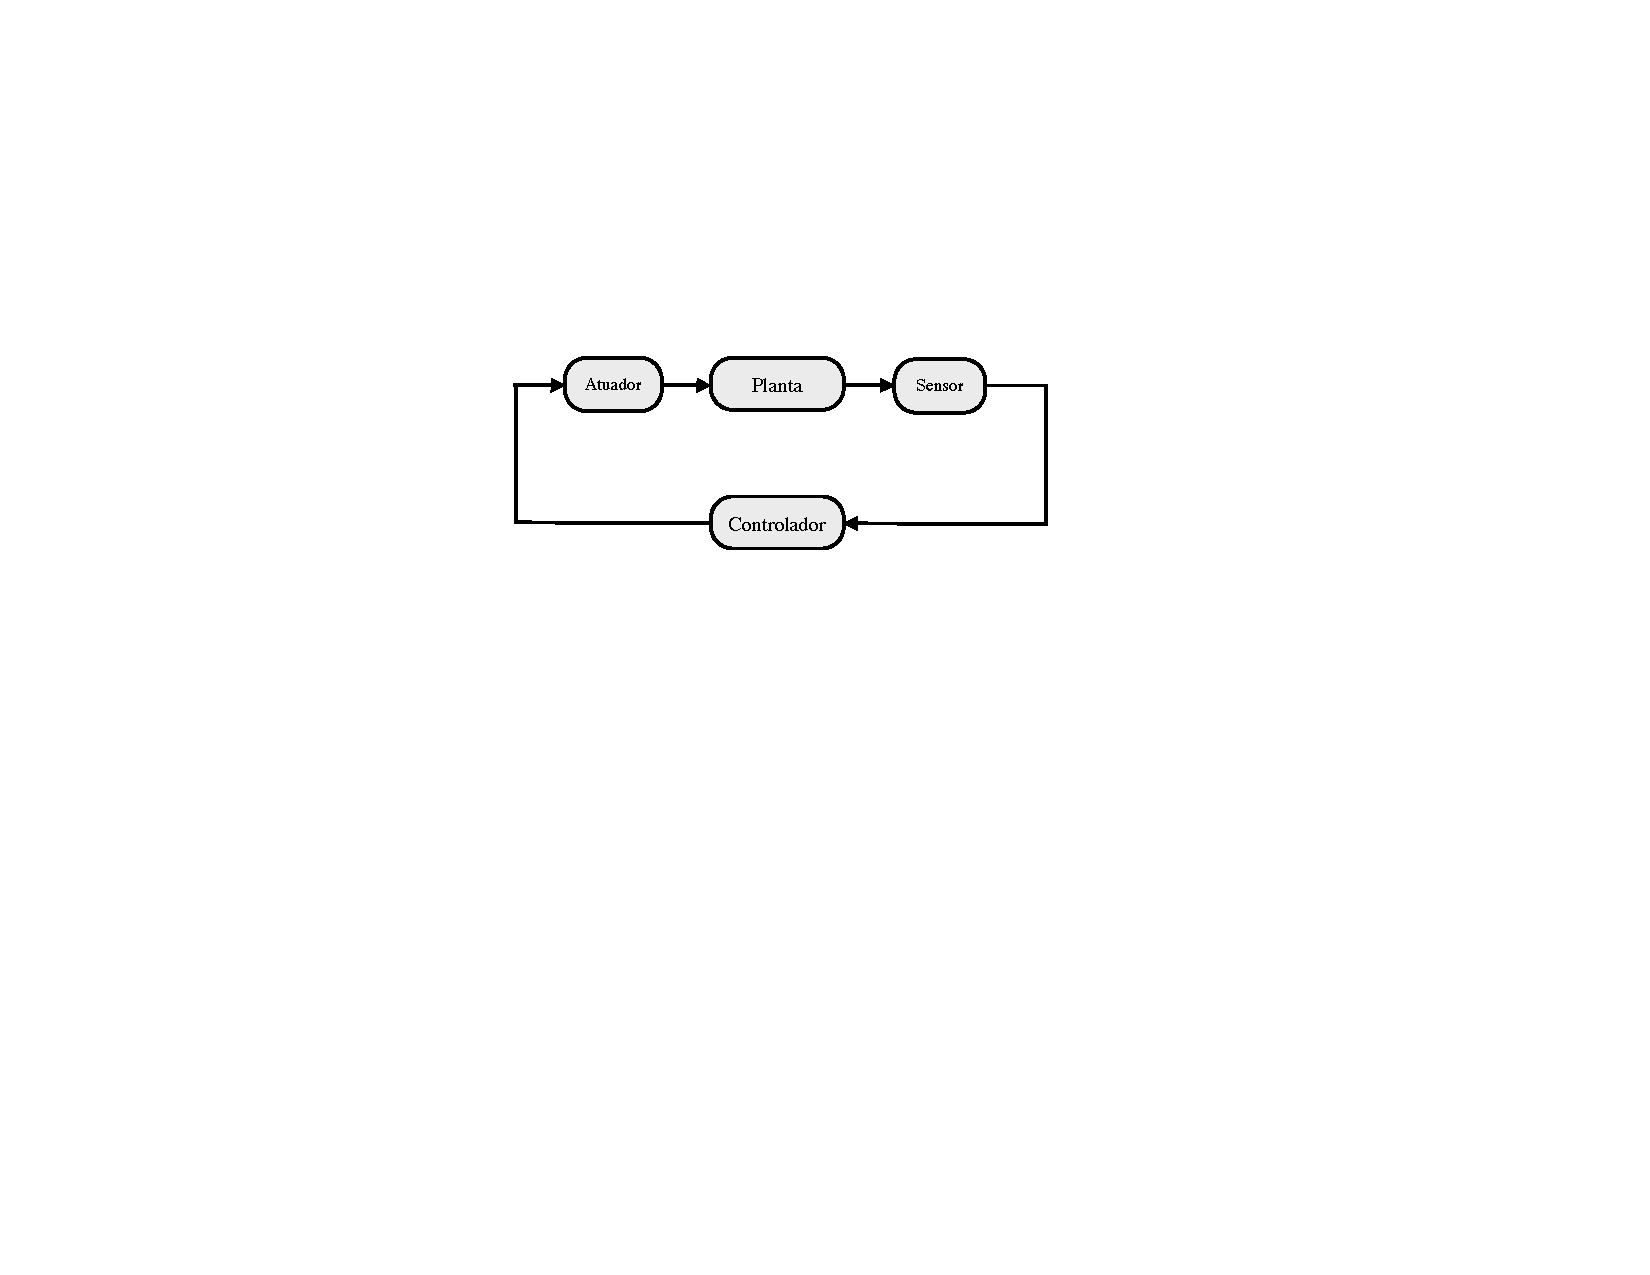
\includegraphics{DescricaoProcesso/Figuras/FiguraProcesso.pdf}}
  \caption{Aqui escrevemos \textbf{toda} informação pertinente à figura. Ou seja, este texto deve ser uma descrição auto-contida da figura, não sendo necessário recorrer ao corpo de texto para saber detalhes sobre a mesma. \emph{Fonte:} Citar fonte se figura 	não for elaborada pelo autor e \textbf{pedir permissão para usar!}}
  \label{fig:processo}
\end{figure}


\section{Situação Atual/Estado da Arte/Revisão da Literatura}
\label{sec:revisão}

Este é o espaço para uma revisão detalhada do enquadramento do problema. Isso inclui descrever a situação atual do processo, aquilo que foi feito até então dentro da empresa/laboratório, e aquilo que se pode chamar de ``Estado da Arte'', ou seja, uma apresentação do conhecimento preexistente
sobre o tema do projeto.

A elaboração desta seção tipicamente demanda uma boa revisão da literatura. Deve haver, quando aplicável uma análise das soluções potencialmente concorrentes, elencando vantagens e desvantagens.

\subsection{Como Elaborar uma Revisão da Literatura}

Ao selecionar referências, devem-se preferir referências de veículos confiáveis, que tenham por exemplo processo de revisão por pares. Portanto, dá-se preferência a artigos em periódicos e livros, em seguida teses e dissertações, artigos em anais de congresso e por fim relatórios. Evitar citar páginas da internet por oferecem menor garantia da informação nelas contida. 

Pesquise sua bibliografia em bases confiáveis como o \textsf{Web of Science}, \textsf{Scopus}, ou o \textsf{Google Scholar}. \textbf{Não use uma ferramenta de busca comum!} (elas não foram feitas pensando no \emph{ranking} de textos científicos) Use o número de citações de uma dada referência como um indicador de sua qualidade. Explore os artigos que citam a referência estudada bem como os artigos que ela cita.

Prefira as referências mais recentes quando se tratar de um assunto na fronteira do conhecimento ou de tecnologia de ponta. Quando se tratar de um assunto já consolidado, prefira citar livros ou artigos com muitas citações. 

Evite citar informações de segunda-mão e procure na medida do possível rastrear a fonte original. Contudo, em situações em que a fonte original é de acesso mais difícil, seja por ter tido publicação limitada como no caso de relatórios ou por não ser em língua inglesa ou portuguesa, é preferível a citação de segunda-mão em um veículo mais acessível.

Para gerenciar suas referências, use uma ferramenta de software como o \textsf{Mendeley}, que permite gerar arquivos .bib para uso em {\LaTeX} ou simplesmente gerar a lista de referências para uso direto em editores de texto. Em \LaTeX, mais especificamente Bib\TeX, a lista de referências é criada a partir de um arquivo .bib, que é uma espécie de banco de informações bibliográficas em que cada entrada é uma referência associada a uma chave para citação. A lista criada incluirá apenas as referências citadas ao longo do texto, mesmo que haja mais referências no arquivo .bib. As informações bibliográficas no formato Bib\TeX também podem ser obtidas para cada referência em ferramentas como o \textsf{Google Scholar} e então coladas no arquivo .bib.

Na Seção \ref{sec:comocitar} discutiremos como e quando as citações devem ser usadas.

\section{Resumo do Capítulo}

Tente não terminar de forma abrupta. Se for escrever algo aqui, não seja genérico!


\clearpage

\chapter{Metodologia}
\label{chap:metodologia}

\section{A modelagem 3D}
\label{sec:modelagem3d}

Para a realização da modelagem matemática, primeiro foi feito um modelo 3D do robô no software OnShape. As peças modeladas formam o corpo do robô. As rodas, os motores e a esfera não foram impressos em 3D, mas são representados no modelo, como é mostrado na imagem a seguir:

\begin{figure}[H]
    \centering
    \begin{subfigure}[b]{1.0\textwidth}
        \centering
        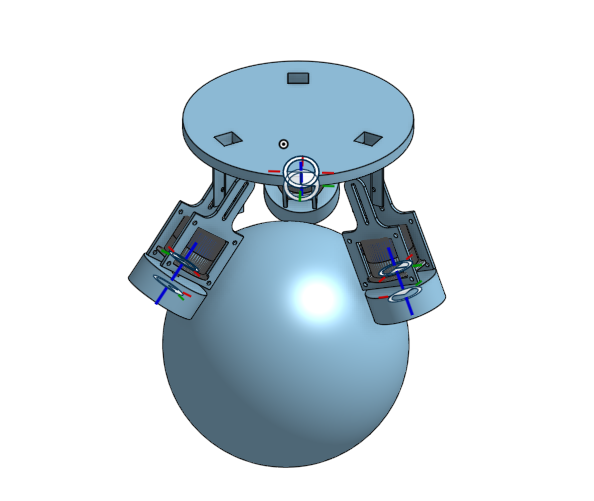
\includegraphics[width=\linewidth]{Metodologia/Figuras/ballbot.png}
        \caption{Modelo 3D}
        \label{fig:modelo_3D}
    \end{subfigure}
\end{figure}

O corpo do robô é um pequeno cilindro, onde são fixados os componentes eletrônicos. Além disso, possui partes que podem se mover para variar o ângulo das rodas e facilitar a acomodação. Essas partes também envolvem a fixação dos motores ao corpo.

\section{A modelagem matemática}
\label{sec:modelagemmatematica}

Para o projeto de controle, fez-se necessário realizar a modelagem mecânica do robô. A etapa seguinte relata como isso foi feito por meio da separação em planos 2D e obtenção das equações de movimento pelo cálculo do Lagrangiano e aplicação das equações de Euler-Lagrange. O passo a passo para realizar os cálculos foi semelhante ao presente no artigo \cite{phdthesis} e adaptado ao modelo projetado.

\subsection{Descrição do modelo}

O robô projetado foi um sistema tridimensional complexo formado por uma esfera, três rodas omnidirecionais e um corpo. Para a representação matemática simplificada, esse modelo foi dividido em três modelos planos independentes (Fig: \ref{fig:modelos_planos}).

\begin{figure}[H]
    \centering
    \begin{subfigure}[b]{0.4\textwidth}
        \centering
        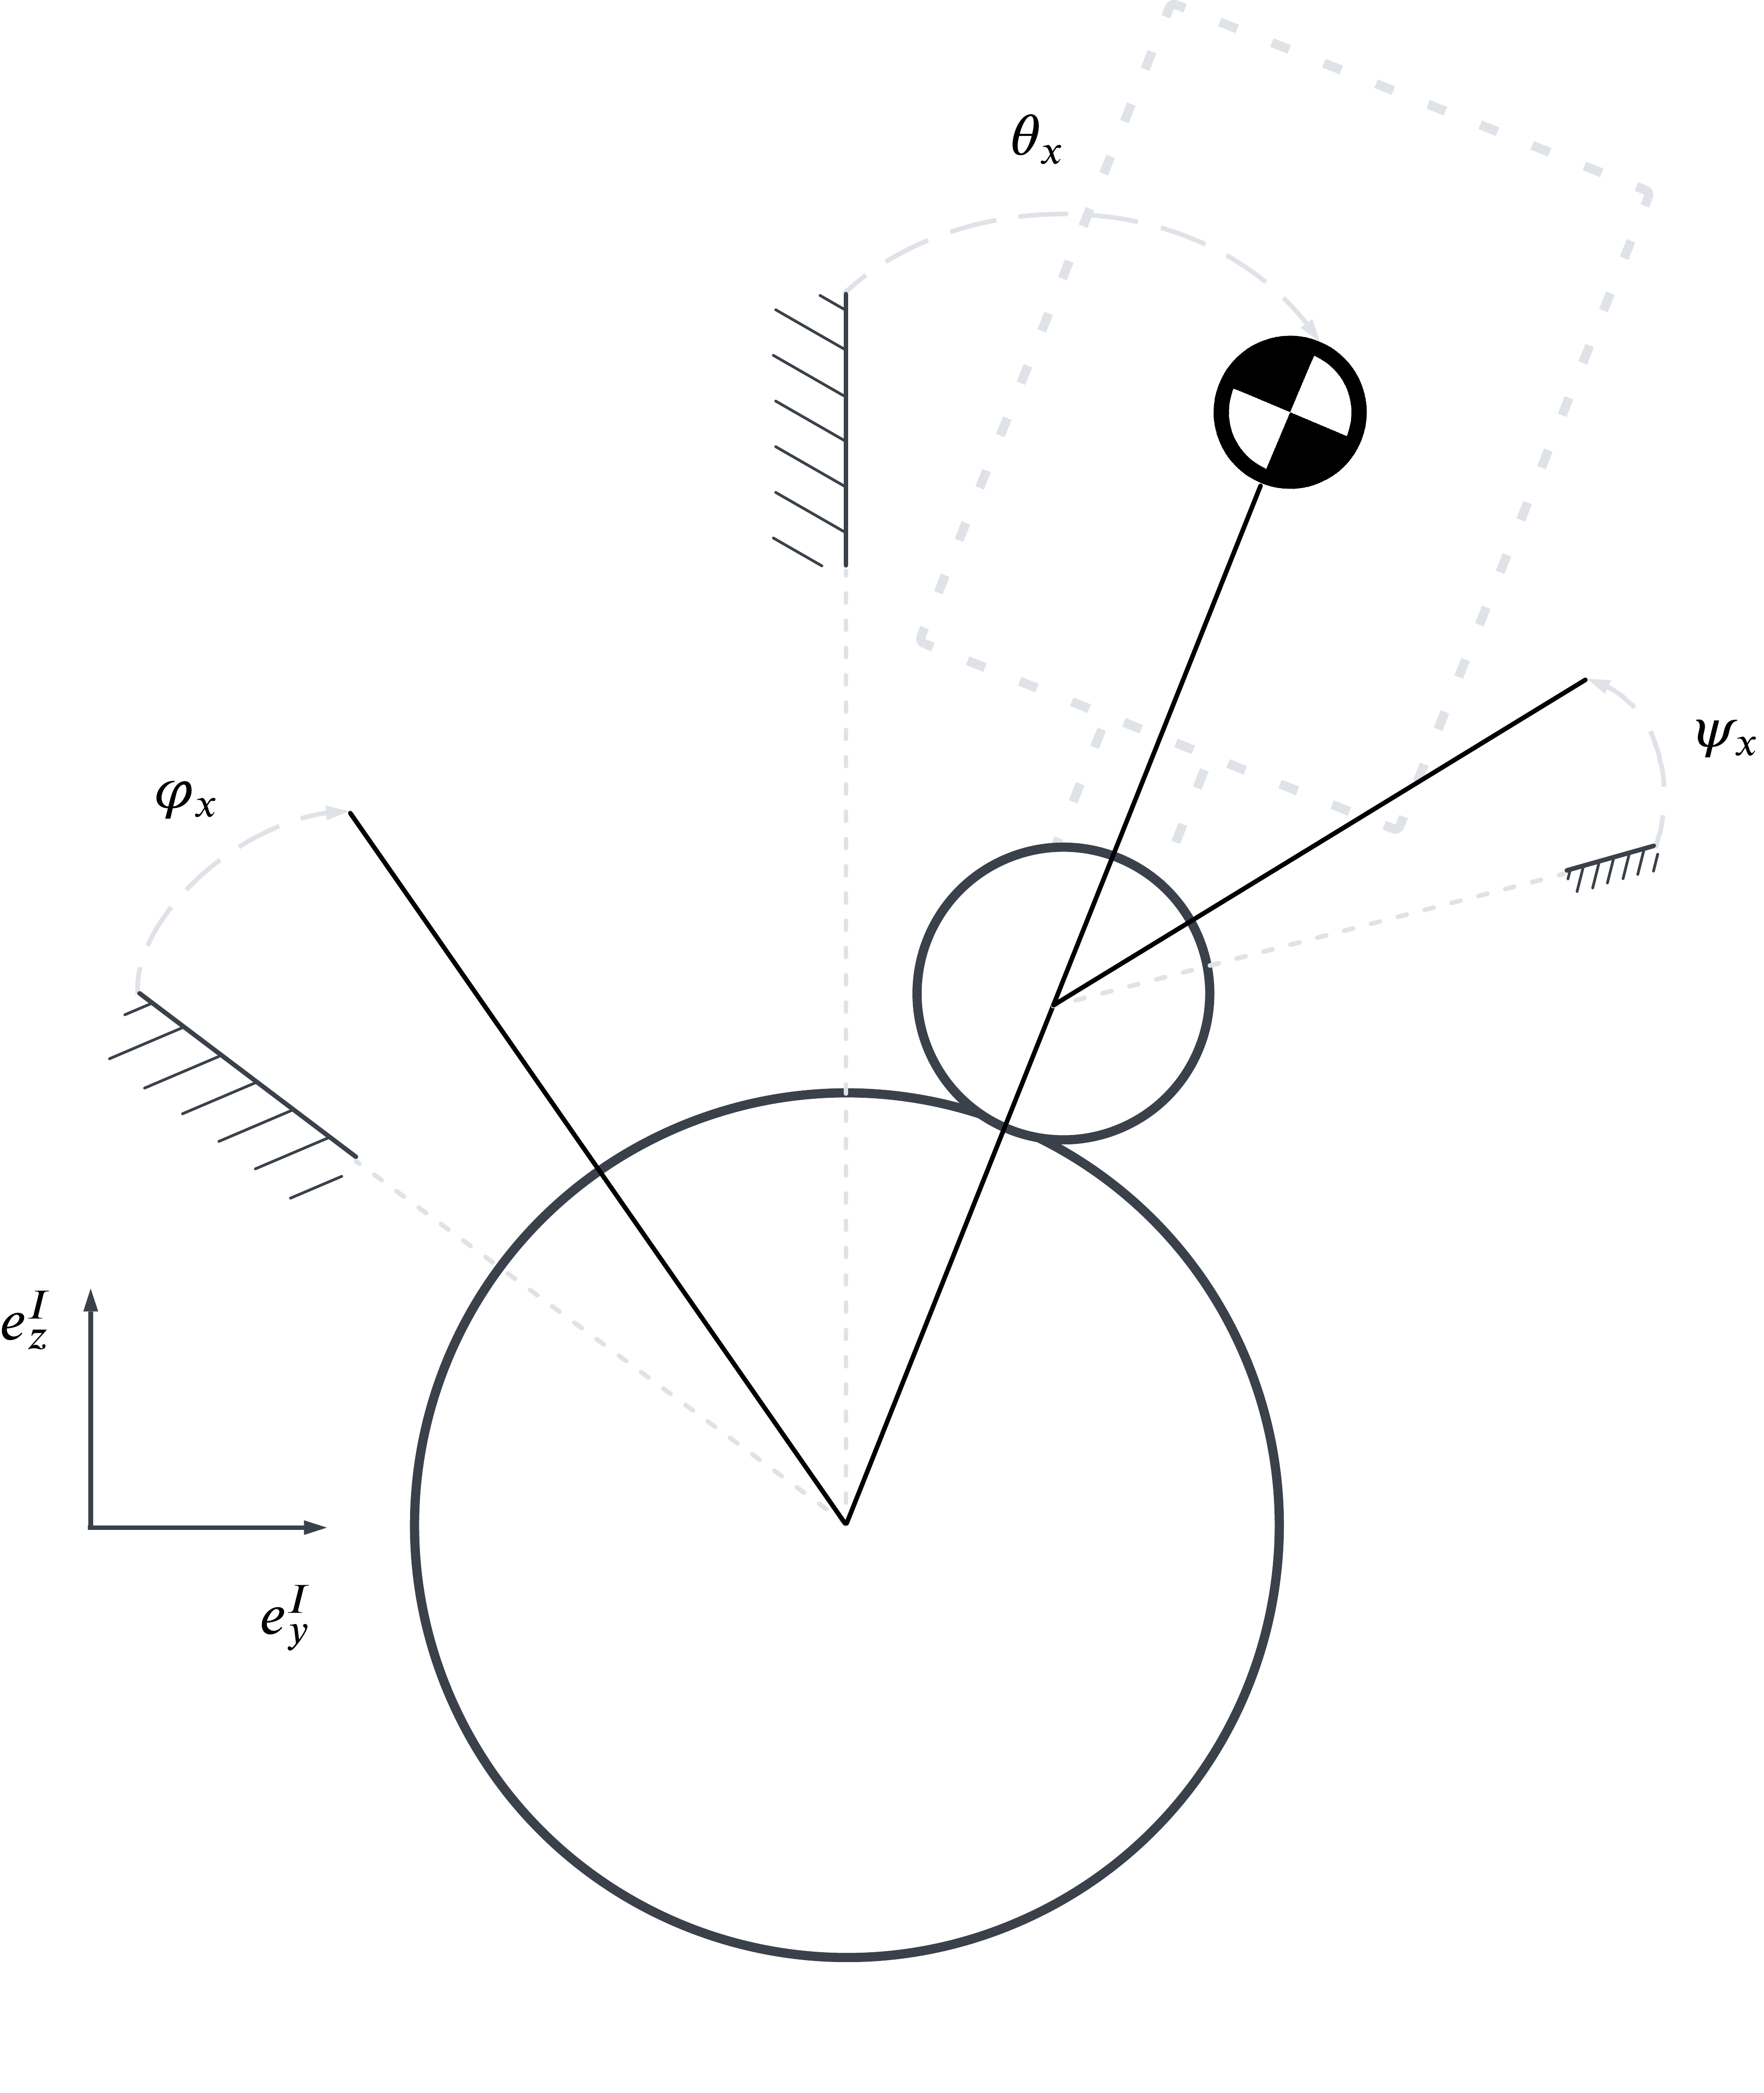
\includegraphics[width=\linewidth]{Metodologia/Figuras/modelo_plano_yz.png}
        \caption{Modelo no plano y-z}
        \label{fig:modelo_yz}
    \end{subfigure}
    \hfill
    \begin{subfigure}[b]{0.4\textwidth}
        \centering
        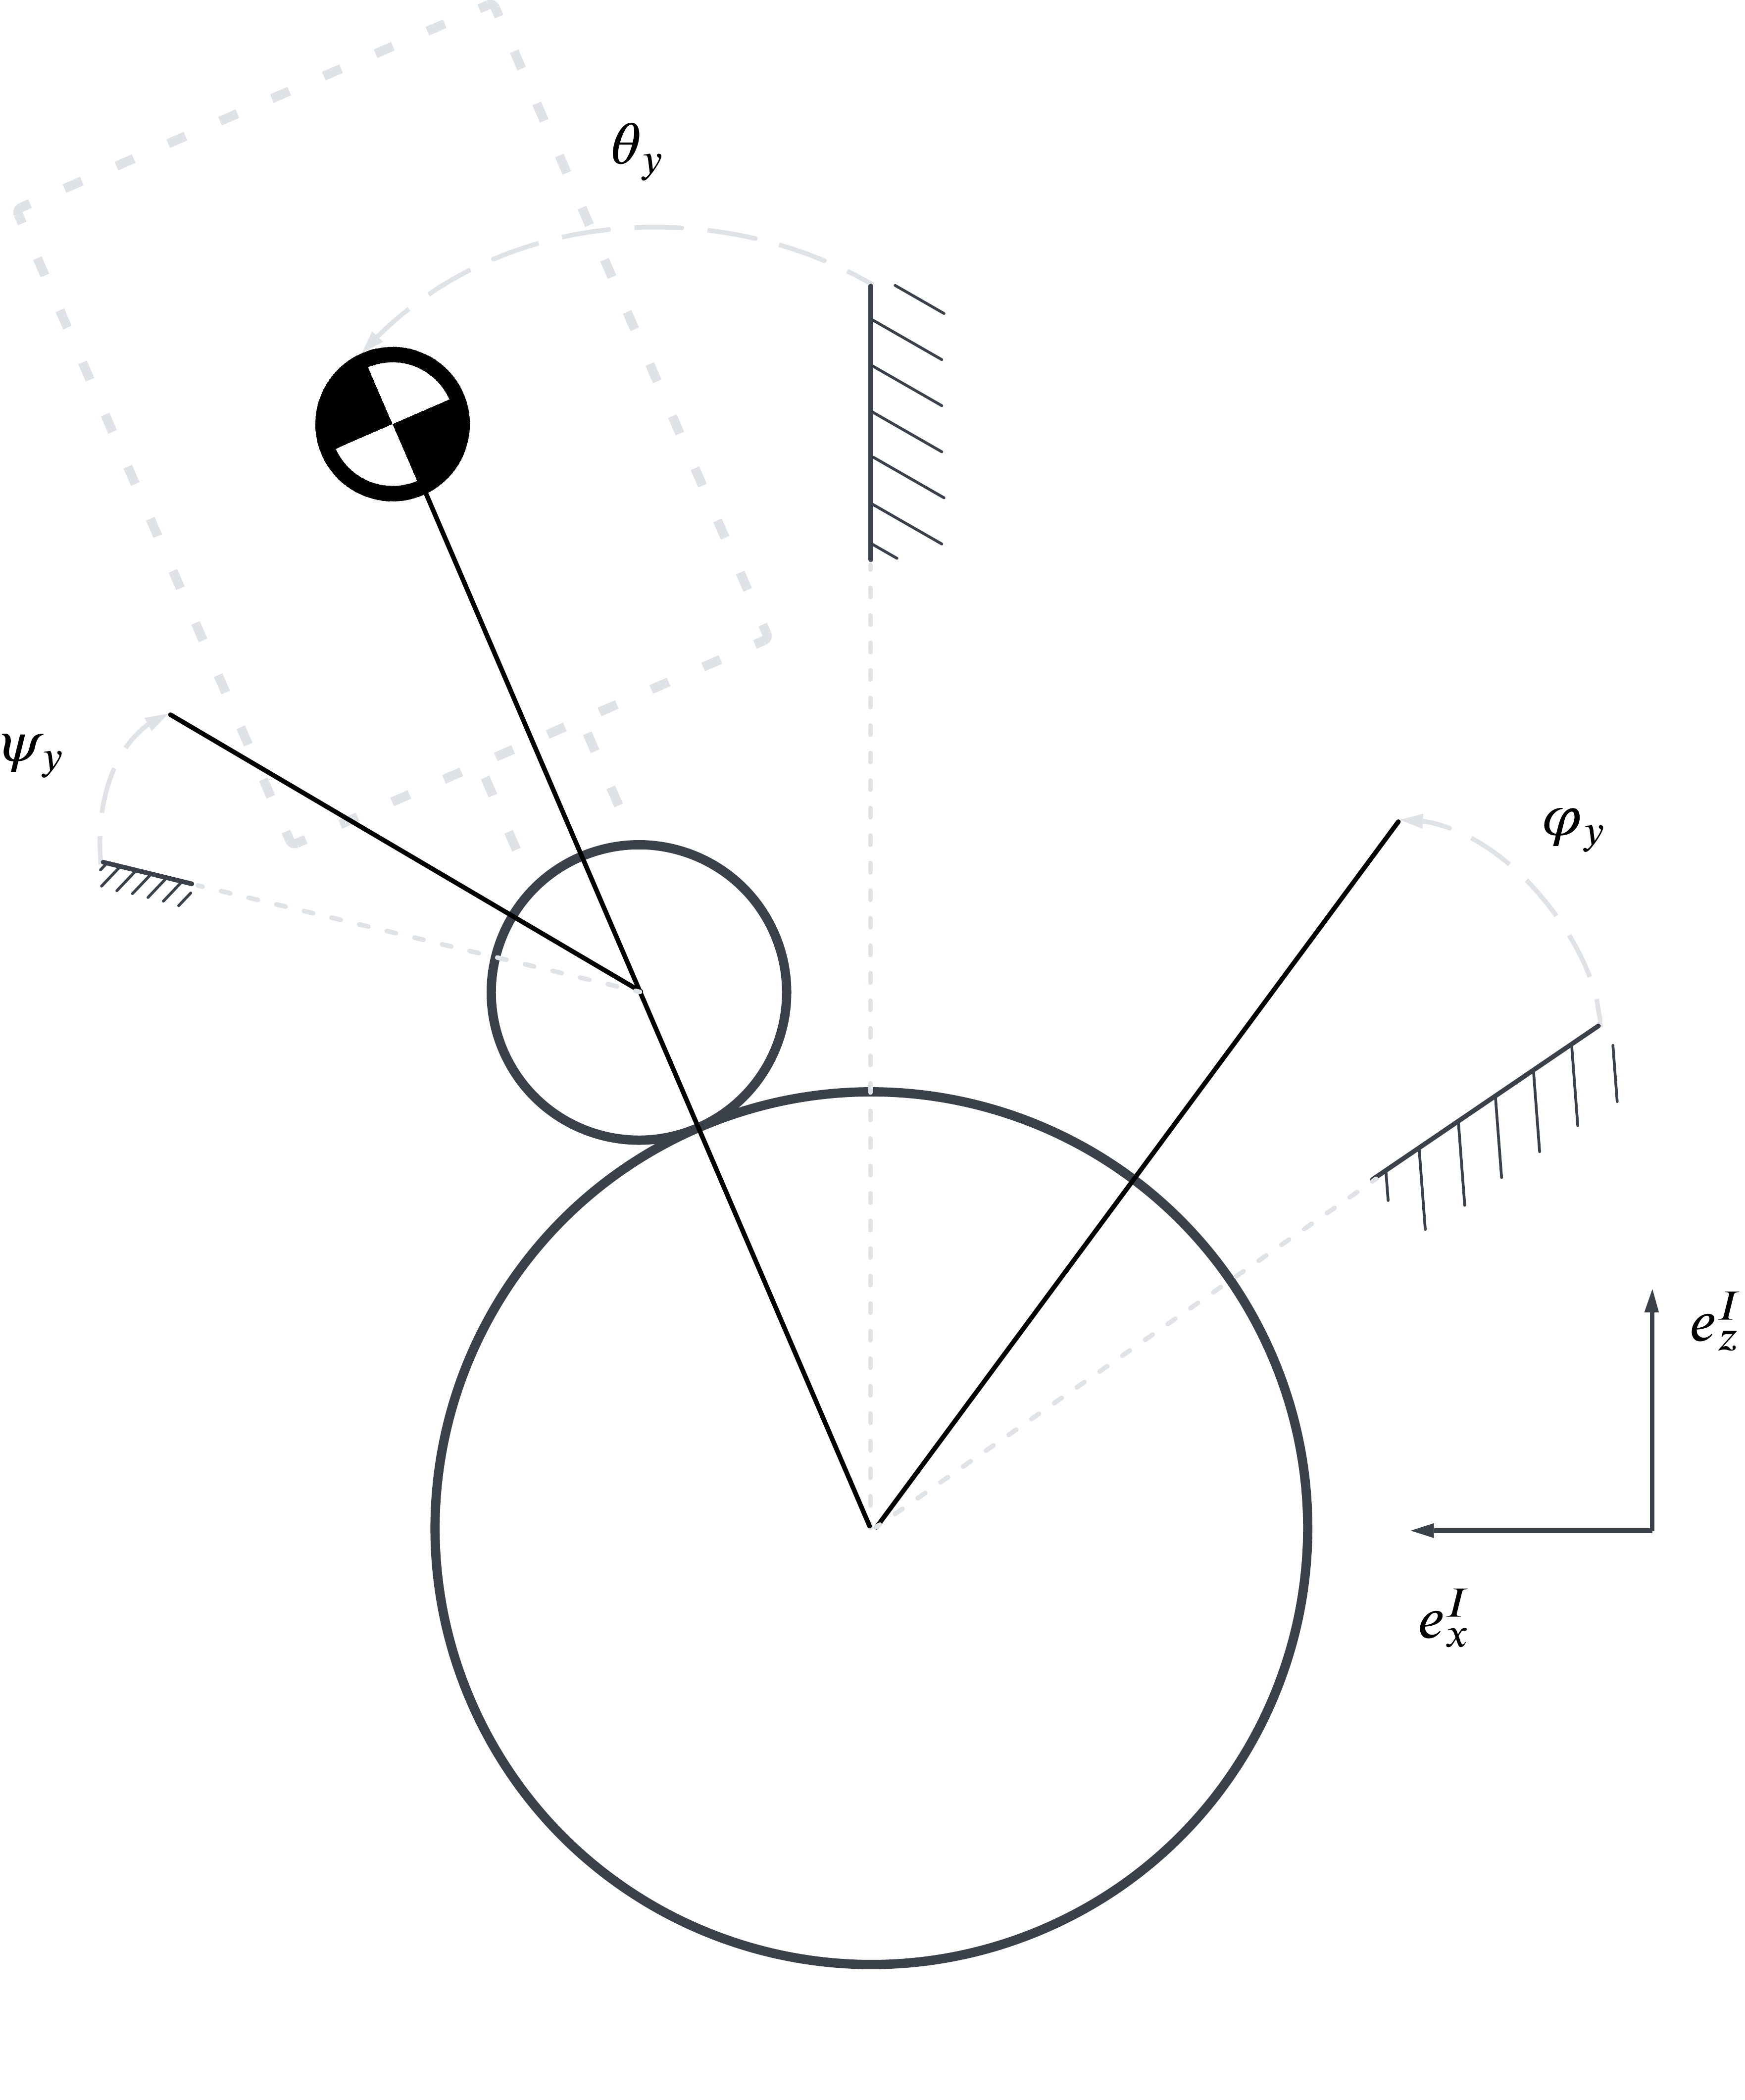
\includegraphics[width=\linewidth]{Metodologia/Figuras/modelo_plano_xz.png}
        \caption{Modelo no plano x-z}
        \label{fig:modelo_xz}
    \end{subfigure}
    \hfill
    \begin{subfigure}[b]{0.4\textwidth}
        \centering
        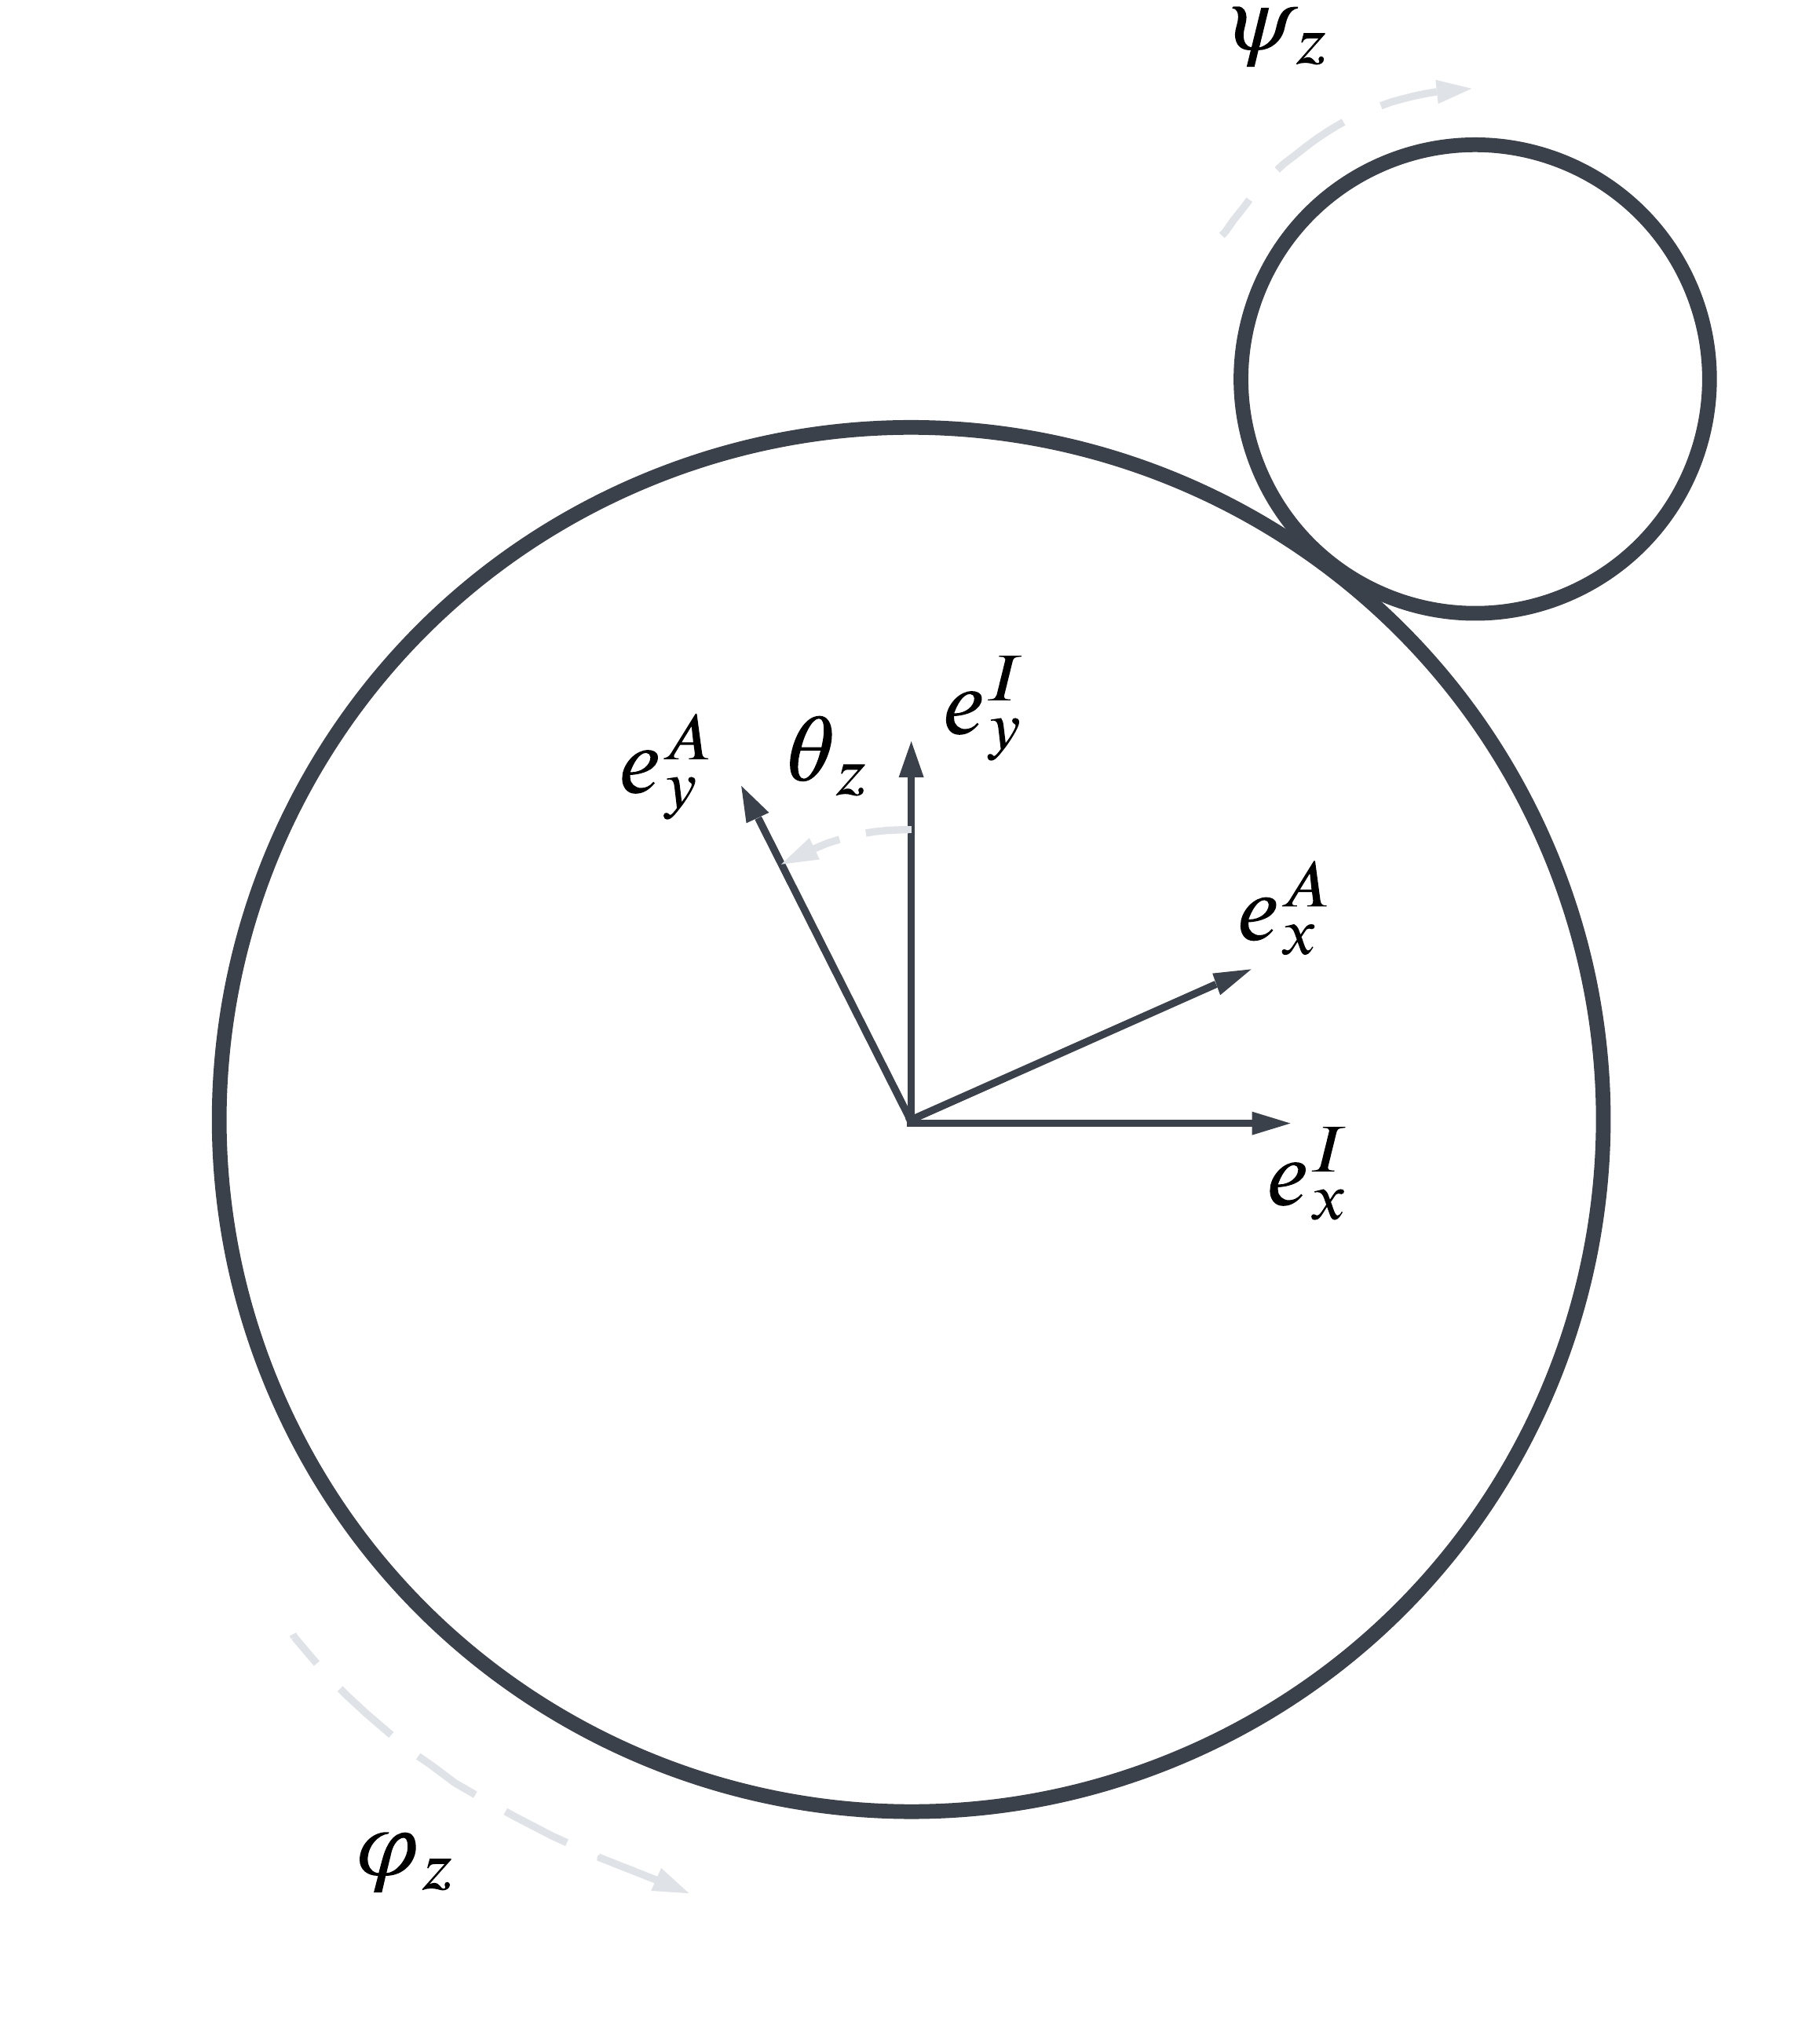
\includegraphics[width=\linewidth]{Metodologia/Figuras/modelo_plano_xy.png}
        \caption{Modelo no plano x-y}
        \label{fig:modelo_xy}
    \end{subfigure}
    \caption{Modelos nos diferentes planos}
    \label{fig:modelos_planos}
\end{figure}

Dessa forma, as três rodas omnidirecionais, que tinham o papel de movimentar o robô, foram transformadas em rodas virtuais, e cada uma foi representada em um modelo. Por causa dessa simplificação, posteriormente foram feitos cálculos para a conversão de posições e velocidades das rodas virtuais para as rodas reais.

\subsection{Suposições}

Os três modelos foram gerados a partir da subdivisão em planos do modelo tridimensional. Consequentemente, os efeitos de acoplamento entre eles foram desconsiderados. Nesse contexto, assumiu-se que o modelo representado no plano $y$-$z$ e o modelo representado no plano $x$-$z$ eram figuras espelhadas uma da outra. Por outro lado, o terceiro modelo, representado no plano $x$-$y$, tinha uma visão única, e apenas descrevia a rotação em torno do eixo \( z \) no sistema de coordenadas fixo do corpo (Fig: \ref{fig:modelo_xy}).

Ademais, com o intuito de simplificar ainda mais os cálculos e garantir a viabilidade do modelo matemático, foram adotadas as seguintes suposições:

\begin{itemize}
    \item Não há deslizamento entre a esfera e a superfície em que o robô está posicionado, assim como entre a esfera e as rodas omnidirecionais.
    \item Apenas o atrito em torno do eixo $z$, entre a esfera e a superfície, foi considerado. Todas as demais forças de atrito foram desconsideradas por serem consideradas irrelevantes.
    \item As interações entre os pontos de contato do robô são idealizadas, ou seja, não há deformações em nenhum desses pontos.
    \item A dinâmica dos motores é significativamente mais rápida do que a dinâmica de estabilização do robô, permitindo que a primeira seja tratada como praticamente instantânea em relação à segunda.
    \item A esfera está restrita a movimentos no plano horizontal, eliminando quaisquer componentes verticais.
\end{itemize}

\subsection{Parâmetros}

O robô possui alguns parâmetros estruturais que foram medidos e estão dispostos na tabela a seguir:

\begin{table}[H]
\centering
\begin{tabular}{|m{6cm}|c|c|c|}
\hline
Parâmetro & Símbolo  & Valor & Unidade de medida \\ \hline
Massa da esfera & $m_K$  & - & $kg$ \\ \hline
Massa da roda & $m_W$  & - & $kg$ \\ \hline
Massa do corpo & $m_A$  & - & $kg$ \\ \hline
Raio da esfera & $r_K$  & - & $m$ \\ \hline
Raio da roda & $r_W$  & - & $m$ \\ \hline
Distância entre o centro da esfera e o centro de massa do corpo & $l$ & - & $m$ \\ \hline
Momento de inércia da esfera & $\Theta_K$  & - & $kg \cdot m^2$ \\ \hline
Momento de inércia da roda nos planos $x$-$z$ e $y$-$z$ & $\Theta_W$  & - & $kg \cdot m^2$ \\ \hline
Momento de inércia da roda no plano $x$-$y$ & $\Theta_{W,xy}$  & - & $kg \cdot m^2$ \\ \hline
Momento de inércia do corpo & $\Theta_{A}$  & - & $kg \cdot m^2$ \\ \hline
Momento de inércia do corpo no plano $x$-$y$ & $\Theta_{A,xy}$  & - & $kg \cdot m^2$ \\ \hline
Ângulo entre o ponto de contato das rodas e o eixo z do sistema de coordenadas da esfera & $\alpha$  & - & $graus$ \\ \hline
Aceleração da gravidade & $g$  & $9,8$ & $\frac{m}{s^2}$ \\ \hline
\end{tabular}
\caption{Parâmetros estruturais}
\label{tab:tabela1}
\end{table}

\subsection{Coordenadas}

Cada um dos modelos foi completamente descrito utilizando os seguintes vetores de coordenadas mínimas:

\begin{equation}
\label{eq:1}
\begin{array}{ccc}
\vec{q_{xy}} =
\begin{bmatrix}
\varphi_z \\
\theta_z
\end{bmatrix}
& 
\vec{q_{yz}} =
\begin{bmatrix}
\varphi_x \\
\theta_x
\end{bmatrix}
& 
\vec{q_{xz}} =
\begin{bmatrix}
\varphi_y \\
\theta_y
\end{bmatrix}
\end{array}
\end{equation}

Onde:

\begin{itemize}
    \item $\varphi_{x,y,z}$: São as orientações da esfera;
    \item $\theta_{x,y,z}$: São as orientações do corpo;
    \item $\psi_{x,y,z}$: São os ângulos das rodas vituais.
\end{itemize}

\subsection{Equações de ligação}

Todas as coordenadas foram expressas utilizando os vetores de coordenadas mínimas e considerando a condição de rolamento sem deslizamento. Para um objeto circular que rola sem deslizar, o deslocamento linear do centro é diretamente proporcional à sua rotação angular, e pode ser calculado pela fórmula:

\begin{equation*}
    \begin{aligned}
        S = r \cdot \theta
    \end{aligned}
\end{equation*}

onde:

\begin{itemize}
    \item \( S \): Deslocamento linear do objeto, medido ao longo do caminho percorrido;
    \item \( r \): Raio do objeto circular;
    \item \( \theta \): Ângulo de rotação do objeto.
\end{itemize}

As coordenadas da esfera, da roda virtual e do centro de massa do corpo no plano $x$-$z$ foram definidas como:

\paragraph{Esfera:}

\begin{equation}
    \label{eq:2}
    \begin{aligned}
        x_K = r_K \cdot \varphi_y,
    \end{aligned}
\end{equation}

\begin{equation}
    \label{eq:3}
    \begin{aligned}
        z_K = 0.
    \end{aligned}
\end{equation}

\paragraph{Roda virtual:}

\begin{equation}
    \label{eq:4}
    \begin{aligned}
        x_W = (r_K \cdot \varphi_y) + (r_K + r_W) \cdot \sin{(\theta_y)},
    \end{aligned}
\end{equation}

\begin{equation}
    \label{eq:5}
    \begin{aligned}
        z_W = (r_K + r_W) \cdot \cos{(\theta_y)}.
    \end{aligned}
\end{equation}

\paragraph{Centro de massa do corpo:}

\begin{equation}
    \label{eq:6}
    \begin{aligned}
        x_A = (r_K \cdot \varphi_y) + l \cdot \sin{(\theta_y)},
    \end{aligned}
\end{equation}

\begin{equation}
    \label{eq:7}
    \begin{aligned}
        z_A = l \cdot \cos{(\theta_y)}.
    \end{aligned}
\end{equation}

Analogamente, foram encontradas as coordenadas no plano $y$-$z$:

\paragraph{Esfera:}

\begin{equation}
    \label{eq:8}
    \begin{aligned}
        y_K = r_K \cdot \varphi_x,
    \end{aligned}
\end{equation}

\begin{equation}
    \label{eq:9}
    \begin{aligned}
        z_K = 0.
    \end{aligned}
\end{equation}

\paragraph{Roda virtual:}

\begin{equation}
    \label{eq:10}
    \begin{aligned}
        y_W = (r_K \cdot \varphi_x) + (r_K + r_W) \cdot \sin{(\theta_x)},
    \end{aligned}
\end{equation}

\begin{equation}
    \label{eq:11}
    \begin{aligned}
        z_W = (r_K + r_W) \cdot \cos{(\theta_x)}.
    \end{aligned}
\end{equation}

\paragraph{Centro de massa do corpo:}

\begin{equation}
    \label{eq:12}
    \begin{aligned}
        y_A = (r_K \cdot \varphi_x) + l \cdot \sin{(\theta_x)},
    \end{aligned}
\end{equation}

\begin{equation}
    \label{eq:13}
    \begin{aligned}
        z_A = l \cdot \cos{(\theta_x)}.
    \end{aligned}
\end{equation}

No modelo do plano $x$-$z$, o ponto $A$ foi definido como o ponto de contato localizado na superfície da esfera, enquanto o ponto $B$ foi definido como o ponto de contato localizado na superfície da roda virtual. Suas velocidades, \( V_A \) e \( V_B \), foram assumidas iguais devido à condição de não deslizamento:

\begin{equation*}
    V_A = V_B \implies 
    \begin{bmatrix}
    V_{Ax} \\
    V_{Az}
    \end{bmatrix} = 
    \begin{bmatrix}
    V_{Bx} \\
    V_{Bz}
    \end{bmatrix}.
\end{equation*}

Substituindo-se os valores chegou-se em:

\begin{equation*}
    \begin{aligned}
        \begin{bmatrix}
        \dot x_K + \dot \varphi_y \cdot r_k \cdot \cos(\theta_y) \\
        \dot \varphi_y \cdot r_K \cdot \sin(\theta_y)
        \end{bmatrix}=
        \begin{bmatrix}
        \dot x_K + (r_K + r_W) \cdot \cos(\theta_y) \cdot \dot \theta_y + \dot \psi_y \cdot r_W \cdot \cos(\theta_y) \\
        - (r_K + r_W) \cdot \sin(\theta_y) \cdot \dot \theta_y + \dot \psi_y \cdot r_W \cdot \sin(\theta_y)
        \end{bmatrix}.
    \end{aligned}
\end{equation*}

Ao se isolar $\dot \psi_y$, obteve-se:

\begin{equation}
    \label{eq:14}
    \begin{aligned}
        \dot \psi_y = \frac{r_K}{r_W} \cdot (\dot \varphi_y - \dot \theta_y) - \dot \theta_y
    \end{aligned}.
\end{equation}

Analogamente, no plano $y$-$z$, foi obtido:

\begin{equation}
    \label{eq:15}
    \begin{aligned}
        \dot \psi_x = \frac{r_K}{r_W} \cdot (\dot \varphi_x - \dot \theta_x) - \dot \theta_x
    \end{aligned}.
\end{equation}

Por fim, utilizando-se o modelo no plano $x$-$y$, as velocidades \( V_A \) e \( V_B \) foram definidas como:

\begin{equation*}
    V_A = 
    \begin{bmatrix}
    V_{Ax} \\
    V_{Ay}
    \end{bmatrix}, \quad 
    V_B = 
    \begin{bmatrix}
    V_{Bx} \\
    V_{By}
    \end{bmatrix}.
\end{equation*}

Assumiu-se novamente \( V_A = V_B \) e se substituíram os valores, obtendo-se:

\begin{equation*}
    \begin{aligned}
        \begin{bmatrix}
        r_K \cdot \sin(\alpha) \cdot \dot \varphi_z \cdot \cos(\theta_z) \\
        r_K \cdot \sin(\alpha) \cdot \dot \varphi_z \cdot \sin(\theta_z)
        \end{bmatrix}=
        \begin{bmatrix}
        r_K \cdot \sin(\alpha) \cdot \dot \theta_z \cdot \cos(\theta_z) + r_W \cdot \dot \psi_z \cdot \cos(\theta_z)\\
        r_K \cdot \sin(\alpha) \cdot \dot \theta_z \cdot \sin(\theta_z) + r_W \cdot \dot \psi_z \cdot \sin(\theta_z)
        \end{bmatrix}.
    \end{aligned}
\end{equation*}

Isolando \( \dot{\psi}_z \), foi obtido:

\begin{equation}
    \label{eq:16}
    \begin{aligned}
        \dot \psi_z = \frac{r_K}{r_W} \cdot \sin(\alpha) \cdot (\dot \varphi_z - \dot \theta_z)
    \end{aligned}.
\end{equation}

\subsection{Energias}

O cálculo das energias potenciais e cinéticas é essencial para a modelagem utilizando o método de Euler-Lagrange. Portanto, para cada modelo planar, esses valores foram calculados como demonstrado a seguir.

\subsubsection{Plano y-z}

\paragraph{Esfera: Energia potencial}

O referencial escolhido se localizava no centro da esfera, logo, a energia potencial nessa situação era nula:

\begin{equation*}
    \begin{aligned}
        V_{K,yz} = 0
    \end{aligned}
\end{equation*}

\paragraph{Esfera: Energia cinética}

A energia cinética foi obtida por meio da soma da parte translacional e da parte rotacional:

\begin{equation*}
    \begin{aligned}
        T_{K,yz} & =\frac{1}{2} \cdot m_K \cdot (r_K \cdot \dot\varphi_x)^2 + \frac{1}{2} \cdot \Theta_K \cdot \dot\varphi_x^2
    \end{aligned}
\end{equation*}

\paragraph{Roda: Energia potencial}

\begin{equation*}
    \begin{aligned}
        V_{W,yz} & = m_W \cdot g \cdot (r_K + r_W) \cdot \cos{(\theta_x)}
    \end{aligned}
\end{equation*}

\paragraph{Roda: Energia cinética}

\begin{equation*}
    \begin{aligned}
        T_{W,yz} & = \frac{1}{2} \cdot m_W \cdot 
        \begin{bmatrix}
            \dot x_W \\
            \dot y_W \\
            \dot z_W
        \end{bmatrix}^T
        \cdot
        \begin{bmatrix}
            \dot x_W \\
            \dot y_W \\
            \dot z_W
        \end{bmatrix}
        +
        \frac{1}{2} \cdot \Theta_W \cdot \dot {\psi_x}^2
    \end{aligned}
\end{equation*}

Os valores de $x_W$, $y_W$ e $z_W$ são:

\begin{equation*}
\scalebox{0.85}{$
    \begin{aligned}
        \begin{bmatrix}
            x_W \\
            y_W \\
            z_W
        \end{bmatrix} 
        & =
        \begin{bmatrix}
            0 \\
            (\varphi_x \cdot r_K ) + (r_K + r_W) \cdot \sin(\theta_x) \\
            (r_K + r_W) \cdot \cos(\theta_x)
        \end{bmatrix}
        \implies
        \begin{bmatrix}
            \dot x_W \\
            \dot y_W \\
            \dot z_W
        \end{bmatrix}
        & =
        \begin{bmatrix}
            0 \\
            (\dot \varphi_x \cdot r_K ) + (r_K + r_W) \cdot \cos({\theta_x}) \cdot \dot \theta_x \\
            - (r_K + r_W) \cdot \sin({\theta_x}) \cdot \dot \theta_x
        \end{bmatrix}.
    \end{aligned}
    $}
\end{equation*}.

Ao substituir esse resultado na equação anterior, obteve-se:

\begin{equation*}
    \scalebox{0.65}{$
        \begin{aligned}
            T_{W,yz} = \frac{1}{2} \cdot m_W \cdot \Big[ (\dot{\varphi}_x \cdot r_K)^2 + 2 \cdot (\dot{\varphi}_x \cdot r_K) \cdot (r_K + r_W) \cdot \cos(\theta_x) \cdot \dot{\theta}_x + (r_K + r_W)^2 \cdot \dot{\theta}_x^2 \Big] + \frac{1}{2} \cdot \Theta_W \cdot \bigg(\frac{r_K}{r_W} \cdot (\dot{\varphi}_x - \dot{\theta}_x) - \dot{\theta}_x \bigg)^2
        \end{aligned}
    $}
\end{equation*}


\paragraph{Corpo: Energia potencial}

\begin{equation*}
    \begin{aligned}
        V_{A,yz} & = m_A \cdot g \cdot l \cdot \cos{(\theta_x)}
    \end{aligned}
\end{equation*}

\paragraph{Corpo: Energia cinética}

\begin{equation*}
    \begin{aligned}
        T_{A,yz} & = \frac{1}{2} \cdot m_A \cdot 
        \begin{bmatrix}
            \dot x_A \\
            \dot y_A \\
            \dot z_A
        \end{bmatrix}^T
        \cdot
        \begin{bmatrix}
            \dot x_A \\
            \dot y_A \\
            \dot z_A
        \end{bmatrix}
        +
        \frac{1}{2} \cdot \Theta_A \cdot \dot {\theta_x}^2
    \end{aligned}
\end{equation*}

Os valores de $x_A$, $y_A$ e $z_A$ são:

\begin{equation*}
    \begin{aligned}
        \begin{bmatrix}
            x_A \\
            y_A \\
            z_A
        \end{bmatrix} 
        & =
        \begin{bmatrix}
            0 \\
            (\varphi_x \cdot r_K ) + l \cdot \sin(\theta_x) \\
            l \cdot \cos(\theta_x)
        \end{bmatrix}
        \implies
        \begin{bmatrix}
            \dot x_A \\
            \dot y_A \\
            \dot z_A
        \end{bmatrix}
        & =
        \begin{bmatrix}
            0 \\
            (\dot \varphi_x \cdot r_K ) + l \cdot \cos({\theta_x}) \cdot \dot \theta_x \\
            - l \cdot \sin({\theta_x}) \cdot \dot \theta_x
        \end{bmatrix}.
    \end{aligned}
\end{equation*}.

Ao substituir esse resultado na equação anterior, foi obtido:

\begin{equation*}
    \begin{aligned}
        T_{A,yz} = \frac{1}{2} \cdot m_A \cdot \Big[ (\dot{\varphi}_x \cdot r_K)^2 + 2 \cdot (\dot{\varphi}_x \cdot r_K) \cdot l \cdot \cos(\theta_x) \cdot \dot{\theta}_x + l^2 \cdot \dot{\theta}_x^2 \Big] + \frac{1}{2} \cdot \Theta_A \cdot \dot \theta_x^2
    \end{aligned}
\end{equation*}

\subsubsection{Plano x-z}

As equações do plano x-z são análogas às equações do plano y-z.

\paragraph{Esfera: Energia potencial}

\begin{equation*}
    \begin{aligned}
        V_{K,xz} = 0
    \end{aligned}
\end{equation*}

\paragraph{Esfera: Energia cinética}

\begin{equation*}
    \begin{aligned}
        T_{K,xz} & = \frac{1}{2} \cdot m_K \cdot (r_K \cdot \dot\theta_y)^2 + \frac{1}{2} \cdot \Theta_K \cdot \dot\theta_y^2
    \end{aligned}
\end{equation*}

\paragraph{Roda: Energia potencial}

\begin{equation*}
    \begin{aligned}
        V_{W,xz} & = m_W \cdot g \cdot (r_K + r_W) \cdot \cos{(\theta_y)}
    \end{aligned}
\end{equation*}

\paragraph{Roda: Energia cinética}

\begin{equation*}
    \scalebox{0.65}{$
    \begin{aligned}
        T_{W,xz} = \frac{1}{2} \cdot m_W \cdot \Big[ (\dot{\varphi}_y \cdot r_K)^2 
        + 2 \cdot (\dot{\varphi}_y \cdot r_K) \cdot (r_K + r_W) \cdot \cos(\theta_y) \cdot \dot{\theta}_y + (r_K + r_W)^2 \cdot \dot{\theta}_y^2 \Big] + \frac{1}{2} \cdot \Theta_W \cdot \bigg(\frac{r_K}{r_W} \cdot (\dot{\varphi}_y - \dot{\theta}_y) - \dot{\theta}_y \bigg)^2
    \end{aligned}
    $}
\end{equation*}

\paragraph{Corpo: Energia potencial}

\begin{equation*}
    \begin{aligned}
        V_{A,xz} & = m_A \cdot g \cdot l \cdot \cos{(\theta_y)}
    \end{aligned}
\end{equation*}

\paragraph{Corpo: Energia cinética}

\begin{equation*}
    \begin{aligned}
        T_{A,xz} = \frac{1}{2} \cdot m_A \cdot \Big[ (\dot{\varphi}_y \cdot r_K)^2 + 2 \cdot (\dot{\varphi}_y \cdot r_K) \cdot l \cdot \cos(\theta_y) \cdot \dot{\theta}_y + l^2 \cdot \dot{\theta}_y^2 \Big] + \frac{1}{2} \cdot \Theta_A \cdot \dot \theta_y^2
    \end{aligned}
\end{equation*}

\subsubsection{Plano x-y}

\paragraph{Esfera: Energia cinética}

\begin{equation*}
    \begin{aligned}
        T_{K,xy} & = \frac{1}{2} \cdot \Theta_K \cdot \dot {\varphi_z}^2 
    \end{aligned}
\end{equation*}

\paragraph{Roda: Energia cinética}

\begin{equation*}
    \begin{aligned}
        T_{W,xy} & = \frac{1}{2} \cdot \Theta_{W,xy} \cdot \dot {\psi_z}^2 
    \end{aligned}
\end{equation*}

\paragraph{Corpo: Energia cinética}

\begin{equation*}
    \begin{aligned}
        T_{A,xy} & = \frac{1}{2} \cdot \Theta_{A,xy} \cdot \dot {\theta_z}^2 
    \end{aligned}
\end{equation*}

\subsection{Torques externos}

As forças não-potenciais \( \vec{f}_{NP} \) representam as forças externas atuando em um sistema. Neste caso, o torque do motor \( T_x \), ou seja, a entrada do sistema, é uma força não potencial. O torque do motor afeta diretamente a coordenada \( \psi_x \). Usando a equação \ref{eq:15}, o efeito do torque do motor nas coordenadas mínimas pode ser expresso como:

\begin{equation}
\label{eq:17}
\vec{f}_{NP,yz1} = 
\begin{bmatrix}
\frac{r_K}{r_W} \cdot T_x \\
-\left(1 + \frac{r_K}{r_W}\right) T_x
\end{bmatrix}
\end{equation}

O torque oposto que atua na coordenada \( \vartheta_x \) do corpo é expresso como:

\begin{equation}
\label{eq:18}
\vec{f}_{NP,yz2} =
\begin{bmatrix}
0 \\
T_x
\end{bmatrix}
\end{equation}

A força total não potencial é então a soma de \( \vec{f}_{NP,yz1} \) e \( \vec{f}_{NP,yz2} \). Um procedimento semelhante é aplicado no plano \( x \)-\( y \). Neste modelo, uma força adicional de atrito \( T_f \) atua em \( \varphi_z \), assim como na rotação da bola:

\begin{equation}
\label{eq:19}
\vec{f}_{NP,xy} =
\begin{bmatrix}
-T_f + \frac{r_K}{r_W} \sin{\alpha} \cdot T_z \\
-\frac{r_K}{r_W} \sin{\alpha} \cdot T_z + T_z
\end{bmatrix}
\end{equation}

\subsection{Equações de movimento}

\begin{equation*}
    \frac{d}{dt} \left( \frac{\partial T}{\partial \dot{\vec{q}}} \right)^T - \left( \frac{\partial T}{\partial \vec{q}} \right)^T + \left( \frac{\partial V}{\partial \vec{q}} \right)^T - \vec{f}_{NP} = 0.
\end{equation*}

$T$ e $V$ são, respectivamente, as energias cinéticas e as energias potenciais.

\begin{equation*}
    T = T_K + T_W + T_A
\end{equation*}
\begin{equation*}
    V = V_K + V_W + V_A
\end{equation*}

As equações de movimento do plano $y$-$z$ podem ser escritas na forma matricial.

\begin{equation*}
M_x(\vec{q}, \dot{\vec{q}}) \ddot{\vec{q}} + C_x(\vec{q}, \dot{\vec{q}}) + G_x(\vec{q}) = f_{NP}
\end{equation*}

As matrizes de inércia, $M_x$, de forças de Coriolis, $C_x$, e de forças gravitacionais, $G_x$, são:

\begin{equation*}
    \begin{aligned}
    M_x &= 
    \begin{bmatrix}
    m_{\text{tot}} r_K^2 + \Theta_K + \left( \frac{r_K}{r_W} \right)^2 \Theta_W & -\frac{r_K}{r_W^2} r_{\text{tot}} \Theta_W + \gamma r_K \cos \vartheta_x \\
    -\frac{r_K}{r_W^2} r_{\text{tot}} \Theta_W + \gamma r_K \cos \vartheta_x & \frac{r_{\text{tot}}^2}{r_W^2} \Theta_W + \Theta_A + m_A l^2 + m_W r_{\text{tot}}^2
    \end{bmatrix}
    \\
    C_x &= 
    \begin{bmatrix}
    -r_K \gamma \sin \vartheta_x \dot{\vartheta}_x^2 \\
    0
    \end{bmatrix}
    \\
    G_x &= 
    \begin{bmatrix}
    0 \\
    -g \sin \vartheta_x \gamma
    \end{bmatrix}
    \end{aligned}
\end{equation*}

Onde:

\begin{equation*}
    \begin{aligned}
        m_{\text{tot}} &= m_K + m_A + m_W \\
        r_{\text{tot}} &= r_K + r_W \\
        \gamma &= l \cdot m_A + (r_K + r_W) m_W
    \end{aligned}
\end{equation*}

A resolução das equações de Lagrange no plano $x$-$y$ para as coordenadas $\ddot{\varphi}_z$ e $\ddot{\vartheta}_z$ produziu:

\begin{equation}
    \label{eq:17}
    \begin{aligned}
    \ddot{\varphi}_z &= 
    -\frac{
    \left( r_W^2 \Theta_{A,xy} + r_K^2 \Theta_{W,xy} \sin^2 \alpha \right) \cdot T_f + r_K r_W \Theta_{A,xy} \sin \alpha \cdot T_z
    }{
    r_W^2 \Theta_{A,xy} \Theta_K + r_K^2 \left( \Theta_{A,xy} + \Theta_K \right) \Theta_{W,xy} \sin^2 \alpha
    }
    \end{aligned}
\end{equation}

\begin{equation}
    \label{eq:18}
    \begin{aligned}
    \ddot{\vartheta}_z &= 
    -\frac{
    r_K \sin \alpha \left( r_K \Theta_{W,xy} \sin \alpha \cdot T_f + r_W \Theta_K \cdot T_z \right)
    }{
    r_W^2 \Theta_{A,xy} \Theta_K + r_K^2 \left( \Theta_{A,xy} + \Theta_K \right) \Theta_{W,xy} \sin^2 \alpha
    }
    \end{aligned}
\end{equation}

Para determinar a força de atrito, considerou-se que a bola permanece constantemente aderida ao solo, satisfazendo a condição de aderência $\ddot\varphi=0$. Assim, com base na equação \ref{eq:17}, $T_f$ foi expresso da seguinte maneira:

\begin{equation*}
    T_f = \frac{r_K r_W \Theta_{A,xy} \sin \alpha \cdot T_z}{r_W^2 \Theta_{A,xy} + r_K^2 \Theta_{W,xy} \sin^2 \alpha}
\end{equation*}

\subsection{Conversão de torques}

Os modelos planares utilizam uma roda virtual para atuar no sistema. O sistema real possui uma estrutura de atuação que difere significativamente daquela assumida no modelo planar. Como um controlador projetado para o modelo planar será implementado no sistema real, é necessário calcular conversões. Para que seja possível controlar o sistema real, os torques nos motores virtuais devem ser convertidos nos torques dos motores reais.

A visão lateral e a visão superior do modelo real estão definidas nas figuras abaixo:

\begin{figure}[H]
    \centering
    \begin{subfigure}[b]{0.4\textwidth}
        \centering
        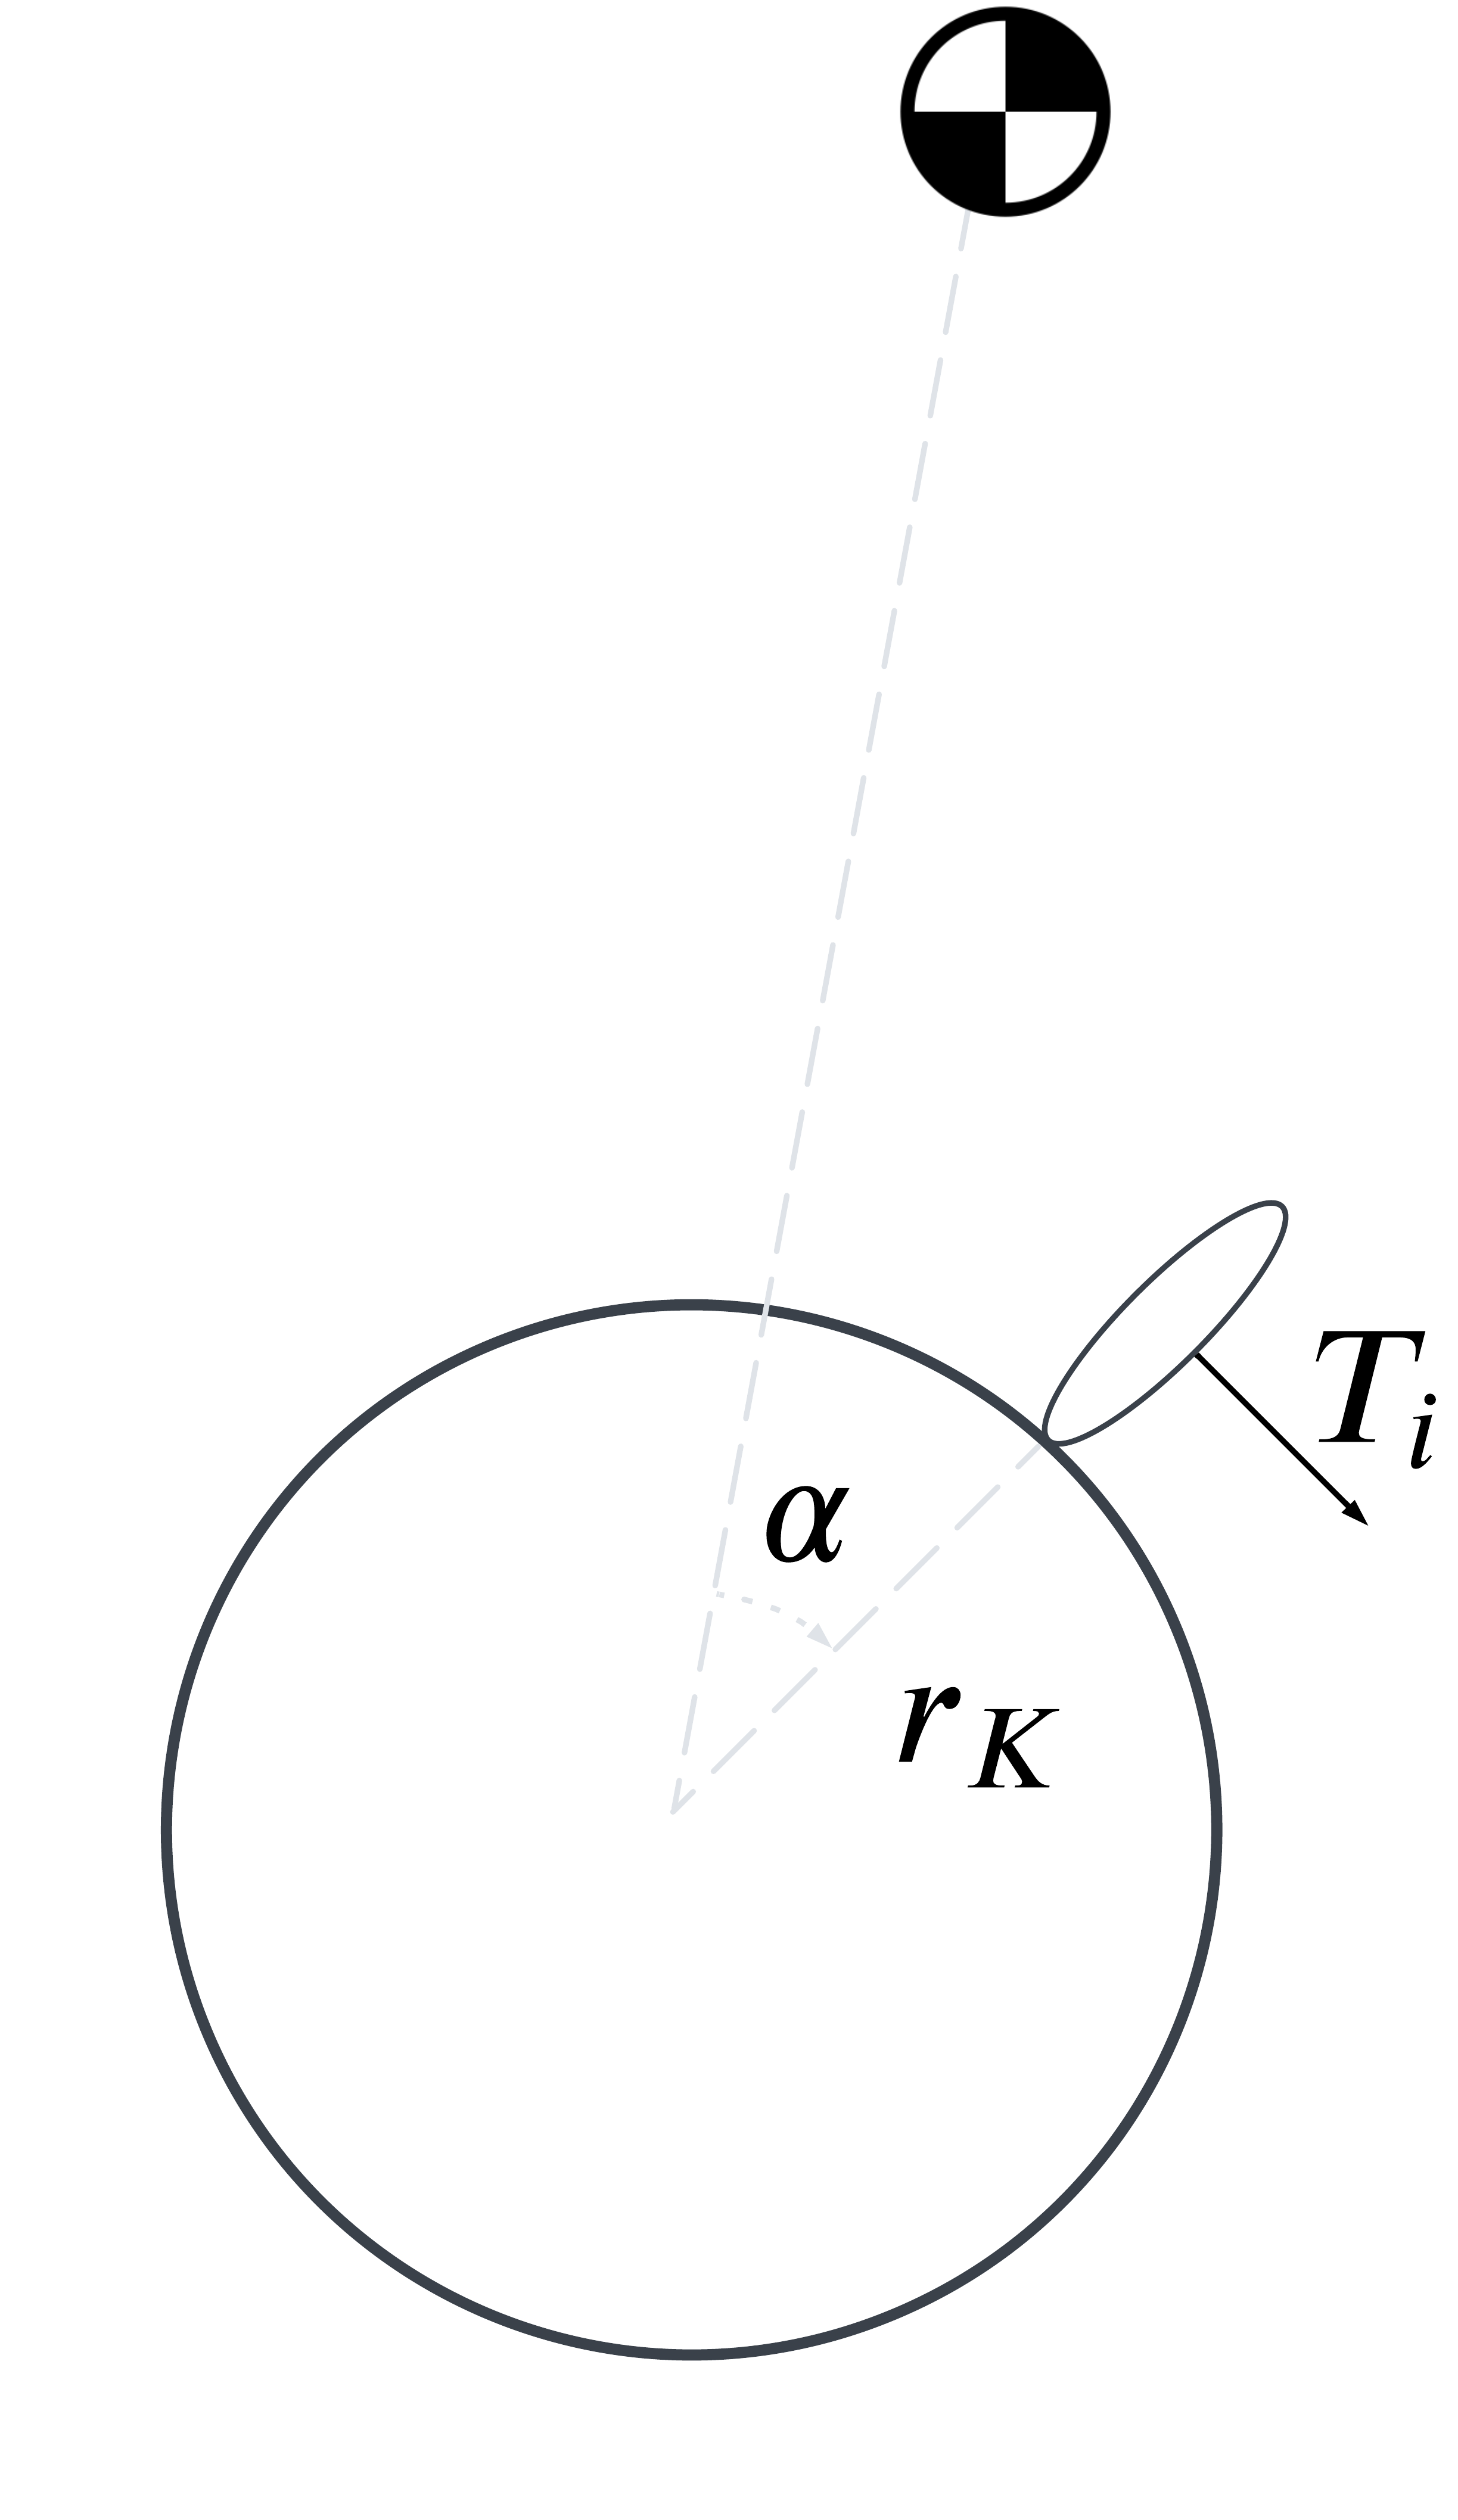
\includegraphics[width=\linewidth]{Metodologia/Figuras/torque_side.png}
        \caption{Modelo real visto de lado}
        \label{fig:torques_lado}
    \end{subfigure}
    \hfill
    \begin{subfigure}[b]{0.4\textwidth}
        \centering
        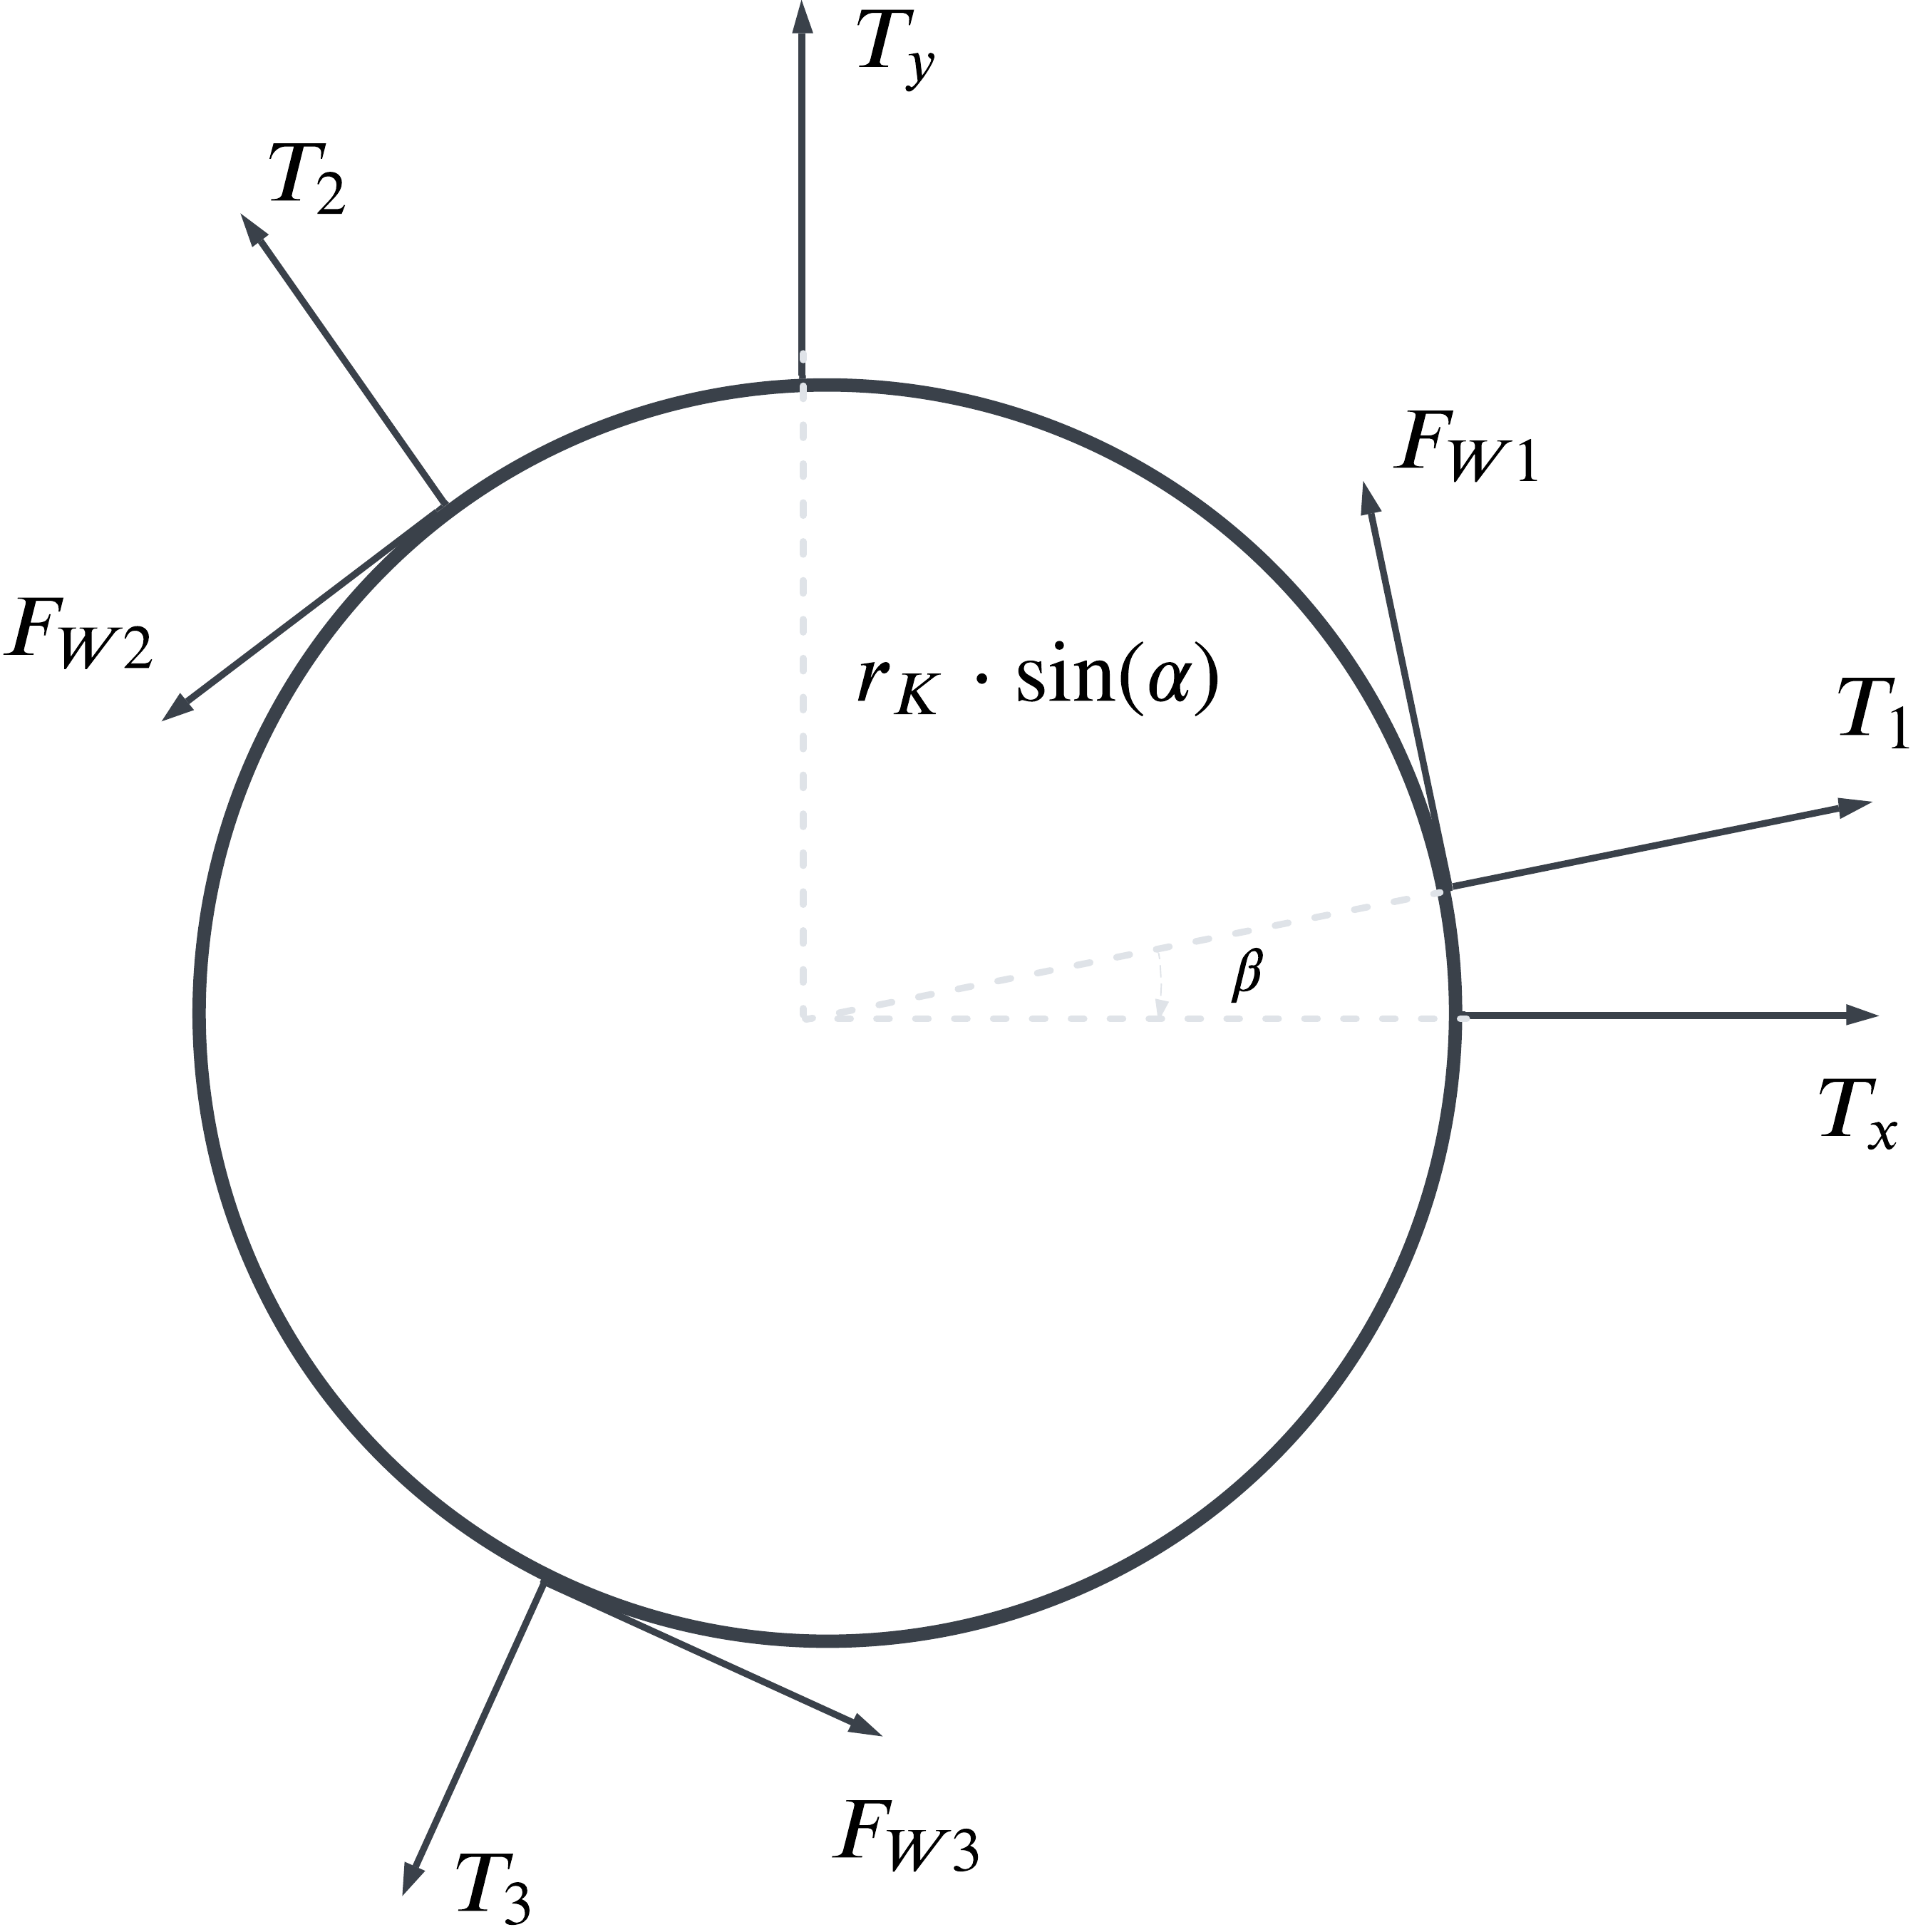
\includegraphics[width=\linewidth]{Metodologia/Figuras/torque_up.png}
        \caption{Modelo real visto de cima}
        \label{fig:torques_cima}
    \end{subfigure}
\end{figure}

Usando esses modelos, obteve-se as forças tangentes provocadas pelo torque dos motores:

\begin{equation}
    \begin{aligned}
    F_{W,1} &= \frac{T_1}{r_W} 
    \begin{bmatrix}
    -\sin \beta \\
    \cos \beta \\
    0
    \end{bmatrix}, \\
    F_{W,2} &= \frac{T_2}{r_W} 
    \begin{bmatrix}
    -\sin \left( \beta + \frac{2}{3}\pi \right) \\
    \cos \left( \beta + \frac{2}{3}\pi \right) \\
    0
    \end{bmatrix}, \\
    F_{W,3} &= \frac{T_3}{r_W} 
    \begin{bmatrix}
    -\sin \left( \beta - \frac{2}{3}\pi \right) \\
    \cos \left( \beta - \frac{2}{3}\pi \right) \\
    0
    \end{bmatrix}.
    \end{aligned}
\end{equation}

Os braços de alavanca também foram obtidos:

\begin{equation}
    \begin{aligned}
        r_{KW,1} &= r_K \cdot 
        \begin{bmatrix}
        \cos \beta \sin \alpha \\
        \sin \beta \sin \alpha \\
        \cos \alpha
        \end{bmatrix}, \\
        r_{KW,2} &= r_K \cdot 
        \begin{bmatrix}
        \cos \left( \beta + \frac{2}{3}\pi \right) \sin \alpha \\
        \sin \left( \beta + \frac{2}{3}\pi \right) \sin \alpha \\
        \cos \alpha
        \end{bmatrix}, \\
        r_{KW,3} &= r_K \cdot 
        \begin{bmatrix}
        \cos \left( \beta - \frac{2}{3}\pi \right) \sin \alpha \\
        \sin \left( \beta - \frac{2}{3}\pi \right) \sin \alpha \\
        \cos \alpha
        \end{bmatrix}.
    \end{aligned}
\end{equation}

Ainda, obteve-se as forças tangentes nos modelos planares e seus braços de alavanca:

\begin{equation}
    \begin{aligned}
    F_{W,x} &= \frac{T_x}{r_W} \cdot 
    \begin{bmatrix}
    0 \\ 
    1 \\ 
    0
    \end{bmatrix}, \\
    F_{W,y} &= \frac{T_y}{r_W} \cdot 
    \begin{bmatrix}
    1 \\ 
    0 \\ 
    0
    \end{bmatrix}, \\
    F_{W,z} &= \frac{T_z}{r_W} \cdot 
    \begin{bmatrix}
    -\sin \beta \\ 
    \cos \beta \\ 
    0
    \end{bmatrix}, \\
    r_{KW,x} = r_{KW,y} &= r_K \cdot 
    \begin{bmatrix}
    0 \\ 
    0 \\ 
    1
    \end{bmatrix}, \\
    r_{KW,z} &= r_K \cdot 
    \begin{bmatrix}
    \cos \beta \cdot \sin \alpha \\ 
    \sin \beta \cdot \sin \alpha \\ 
    0
    \end{bmatrix}.
    \end{aligned}
\end{equation}

Portanto, os torques na bola no modelo real e nos modelos planares são:

\begin{equation}
    \begin{aligned}
    T_{KW,i} &= r_{KW,i} \times F_{W,i} \quad \text{para } i = 1, 2, 3, \\
    T_{KW,j} &= r_{KW,j} \times F_{W,j} \quad \text{para } j = x, y, z.
    \end{aligned}
\end{equation}

Como o torque total deve ser conservado, usou-se a equação

\begin{equation}
    T_{KW,1} + T_{KW,2} + T_{KW,3} = T_{KW,x} + T_{KW,y} + T_{KW,z}
\end{equation}

para calcular o torque dos motores reais e o torque dos motores virtuais:

\begin{align*}
T_1 &= \frac{1}{3} \left( T_z + \frac{2}{\cos \alpha} \cdot \left( T_x \cdot \cos \beta - T_y \cdot \sin \beta \right) \right) \\
T_2 &= \frac{1}{3} \left( T_z + \frac{1}{\cos \alpha} \cdot \left( \sin \beta \cdot \left( -\sqrt{3} T_x + T_y \right) - \cos \beta \cdot \left( T_x + \sqrt{3} T_y \right) \right) \right) \\
T_3 &= \frac{1}{3} \left( T_z + \frac{1}{\cos \alpha} \cdot \left( \sin \beta \cdot \left( \sqrt{3} T_x + T_y \right) + \cos \beta \cdot \left( -T_x + \sqrt{3} T_y \right) \right) \right)
\end{align*}

\begin{align*}
T_x &= \cos \alpha \cdot \left( T_1 \cdot \cos \beta - T_2 \cdot \sin \left( \beta + \frac{\pi}{6} \right) + T_3 \cdot \sin \left( \beta - \frac{\pi}{6} \right) \right) \\
T_y &= \cos \alpha \cdot \left( -T_1 \cdot \sin \beta - T_2 \cdot \cos \left( \beta + \frac{\pi}{6} \right) + T_3 \cdot \cos \left( \beta - \frac{\pi}{6} \right) \right) \\
T_z &= T_1 + T_2 + T_3
\end{align*}

\subsection{Cálculos de inércia}

A inércia da bola foi aproximada por uma esfera oca, 

\begin{equation*}
    \Theta_K = \frac{2}{3} \cdot m_K \cdot r_K^2,
\end{equation*}

enquanto o corpo foi aproximado por um cilindro:

\begin{equation*}
    \Theta_A = \frac{1}{4} \cdot m_A \cdot r_A^2 + \frac{1}{2} \cdot m_A \cdot h^2 + m_A \cdot l^2,
\end{equation*}

\begin{equation*}
    \Theta_{A,xy} = \frac{1}{2} \cdot (m_A + m_W) \cdot r_A^2.
\end{equation*}

Dado o momento de inércia do motor, $\Theta_M$, e o momento de inércia da roda omnidirecional,

\begin{equation}
    \Theta_{OW} = \frac{1}{2} \cdot m_{OW} \cdot r_W^2
\end{equation},

onde $m_{OW}$ é a massa da roda omnidirecional.

Ainda, há o momento de inércia das rodas virtuais, que foi obtido comparando a energia rotacional em torno de um eixo no sistema virtual com a energia rotacional em torno do mesmo eixo no sistema real.

As velocidades angulares da rodas na direção $y$ são:

\begin{align*}
\omega_{OW,1} &= \omega_{W,x} \cos \alpha \\
\omega_{OW,2/3} &= -\frac{1}{2} \omega_{W,x} \cos \alpha
\end{align*}

Enquanto na direção $x$ são:

\begin{align*}
\omega_{OW,1} &= 0 \\
\omega_{OW,2} &= -\frac{\sqrt{3}}{2} \omega_{W,y} \cos \alpha \\
\omega_{OW,3} &= \frac{\sqrt{3}}{2} \omega_{W,y} \cos \alpha
\end{align*}

Por fim, na direção z:

\begin{equation*}
    \omega_{OW,1/2/3} = \omega_{W,z} \sin \alpha
\end{equation*}.

Fazendo o quilibrio energético na direção y,
\begin{align*}
\frac{1}{2} \Theta_{W,x} \dot{\psi}_x^2 &= \frac{1}{2} \Theta_{OW} (\dot{\psi}_x \cos \alpha)^2 + \frac{1}{2} \Theta_M (\dot{\psi}_x \cos \alpha)^2 \\
&\quad + \frac{1}{2} \cdot 2 \left( \Theta_{OW} \left(-\frac{1}{2} \dot{\psi}_x \cos \alpha \right)^2 + \Theta_M \left(-\frac{1}{2} \cdot \dot{\psi}_x \cos \alpha \right)^2 \right) \\
\Theta_{W,x} &= \cos^2(\alpha) \left( \Theta_{OW} + \Theta_M + \frac{1}{2} \left( \Theta_{OW} + \Theta_M \right) \right) \\
&= \frac{3}{2} \cos^2(\alpha) \left( \Theta_{OW} + \Theta_M \right)
\end{align*},

e na direção x,
\begin{align*}
\frac{1}{2} \Theta_{W,y} \dot{\psi}_y^2 &= \frac{1}{2} \cdot 2 \left( \Theta_{OW} \left(\frac{\sqrt{3}}{2} \dot{\psi}_y \cos \alpha \right)^2 + \Theta_M \left(-\frac{\sqrt{3}}{2} \cdot \dot{\psi}_x \cos \alpha \right)^2 \right) \\
\Theta_{W,y} &= \frac{3}{2} \cos^2(\alpha) (\Theta_{OW} + \Theta_M),
\end{align*}

usando a notação.

\begin{align*}
\dot{\psi}_x &= \omega_{W,x} \\
\dot{\psi}_y &= \omega_{W,y} \\
\dot{\psi}_1 &= \omega_{OW,1} \\
\dot{\psi}_2 &= \omega_{OW,2} \\
\dot{\psi}_3 &= \omega_{OW,3}.
\end{align*}

tem-se, portanto,

\begin{align*}
\Theta_{W} = \Theta_{W,x} = \Theta_{W,y} = \frac{3}{2} \cos^2(\alpha) (\Theta_{OW} + \Theta_M).
\end{align*}

Seguindo-se o mesmo procedimento para o plano $x$-$y$ obteve-se:

\begin{align*}
    \Theta_{W,xy} = 3 \cdot (\Theta_{OW} + i^2 \cdot \Theta_M).
\end{align*}


\section{Projeto de controladores}
\label{sec:projetocontroladores}

\clearpage
\chapter{Resultados}

Para a execução do projeto, algumas etapas de desenvolvimento tiveram de ser seguidas: familiarização com o sistema, estudo dos módulos envolvidos, leitura dos requisitos, elaboração de documento descrevendo todo o processo de implementação e relacionamento com os diversos módulos, implementação e testes.


\section{Atividades do Projeto}
\label{metodo3}

\section {Requisitos do Sistema}
\label{req}


\section{Desenvolvimeto e Implementação}

A Tabela \ref{tab:tabela} apresenta as atividades executadas.

\begin{table}
\centering
%Note os alinhamentos diferentes em cada coluna
\begin{tabular}{|c|r|l|}\hline
		Atividade 1 & aa  & ab  \\ 
					 & a & b \\ \hline
		Ativ. 2  & aa & ab \\			
					 &  a & b \\ \hline
		\end{tabular}
	\caption{Exemplo de tabela - Coloque toda informação sobre a tabela aqui}
	\label{tab:tabela}
\end{table}

\section{Testes}

\section{Análise dos Resultados}

Apresente os resultados sem adulterações e faça análises objetivas. Pense na melhor maneira de apresentar os resultados graficamente. Se os gráficos são difíceis de interpretar, talvez tabelas sejam uma forma melhor de apresentar resultados. Não apresente dados (gráficos e tabelas) se não há uma conclusão interessante a ser tirada. Lembre-se de ser conciso.

\emph{Não se esqueça das unidades!} Pense que \emph{a priori} todo número deve ter uma unidade. Não escreva as unidades em itálico (no ambiente matemático) e tome cuidado para diferenciar maiúsculas e minúsculas. Um exemplo é escrever $22$ [kN] e não $22 KN$ (Kelvin vezes Newton!).

Ao apresentar resultados experimentais, tome o cuidado para também apresentar o cálculo das incertezas sempre que forem significativas. Ao fazer conclusões, sempre considere se o tamanho da sua amostra é grande o suficiente do ponto de vista estatístico. Lembre que a média empírica $\hat{\mu}_X$ de $N$ observações independentes da variável $X_i$ possui variância
\[
\hat{\sigma}_{\mu}^2 = \frac{1}{N(N-1)} \sum_{i=1}^N (X_i-\hat{\mu}_X)^2
\enspace,
\]
onde se assume que as variáveis $X_i$ possuem uma mesma ditribuição e que essa distribuição possui segundo momento finito.


\section{Resumo do Capítulo}
\label{sec:resumoo4}
Tente não terminar de forma abrupta. Se for escrever algo aqui, não seja genérico!

\section{Formato, expressões matemáticas e o \LaTeX}

\subsection{O \LaTeX}

O {\LaTeX}  é o método preferencial de preparação de documentos para textos técnicos nas ciências exatas. O {\LaTeX} permite não só lidar com equações de uma forma mais prática que em editores de texto, mas também facilita a formatação de documentos e tem um desempenho marcadamente superior a editores de texto na preparação de documentos longos como monografias. 

Documentos em {\LaTeX} são escritos em um ou mais arquivos de texto com extensão .tex. Após a escrita, o .tex é \emph{compilado} para gerar arquivos nos formatos .pdf, .dvi ou .ps. Hoje há duas distribuições padrão para o \LaTeX. Sistemas Windows usam o {Mik\TeX} e sistemas Unix usam o \TeX Live. Além das distribuições, muitos usuários utilizam \emph{front-ends} que facilitam a edição do texto, a compilação e a instalação de pacotes. 

Os pacotes necessários para compilar o presente documento devem ser encontrados numa instalação completa dessas distribuições. Se tiver dificuldades com os pacotes, você pode instalá-los manualmente ou tentar alterar o código para usar versões antigas dos mesmos.

A compilação pode ser feita pelos comandos \textsf{latex} ou \textsf{pdflatex}, invocados pela linha de comando ou pelo \emph{front-end}. Note que será necessário empregar o comando \textbf{mais de uma vez} para que as referências cruzadas saiam corretas.

Como discutido na Seção \ref{sec:revisão}, uma ferramenta útil para gerenciar as citações em {\LaTeX} é o Bib\TeX. Para gerar uma lista bibliográfica a partir do arquivo .bib, este arquivo deve ser indicado no arquivo .tex. Em seguida devem-se executar os comandos \textsf{pdflatex}, \textsf{bibtex} e \textsf{pdflatex} novamente sempre usando o .tex como argumento. Note que os comandos são executados nesta ordem e de forma repetida para que as referências cruzadas sejam geradas corretamente.

Nesta seção você deve encontrar exemplos dos comandos mais usados em \LaTeX. Outros exemplos e manuais podem ser encontrados na internet com facilidade.

\subsection{Expressões Matemáticas}

Ao escrever expressões matemáticas, defina todas as variáveis antes de usá-las ou imediatamente depois da expressão. Deixar de fazê-lo torna seu texto \textbf{ilegível}. Segue um exemplo.

Seja o par $(a_1,a_2)\in \mathbb{R}^2$. Para $s\in\mathbb{C}$, definimos a função $f(s)$ como
\[%cria equações sem numeração
f(s)\triangleq \frac{a_1 s+a_2}{s^2+2\zeta\omega_n s+\omega_n^2}
\enspace,
\]
onde os escalares $\zeta,\omega_n>0$ são constantes.

Note que não foi necessário atribuir valores às variáveis neste momento. Repare também como devemos \textbf{usar pontuação} (vírgula) nas equações, tratando-as como parte da frase. Usamos o símbolo $\triangleq$ ou $:=$ para deixar explícito que se trata de uma definição. Ser claro nesse aspecto facilita o entendimento do leitor.

A equação acima não foi numerada porque não será citada no texto. Vejamos um exemplo com numeração.

A função $f(\cdot)$ possui um zero em $-a_2/a_1$ (ou $-\frac{a_2}{a_1}$) e, para $\zeta<1$, possui polos complexos $p_{1,2}$ dados por
\begin{equation}
\label{eq:polos}
p_{1,2}=\omega_n \left(-\zeta\pm j\sqrt{1-\zeta^2}\right)
\enspace.
\end{equation}
Agora podemos citar os polos dados pela Equação (\ref{eq:polos}) (aqui adotamos a convenção de citar sempre com o número entre parênteses precedido da palavra Equação). Note como usamos um comando especial na Equação \ref{eq:polos} para garantir o ajuste automático do tamanho dos parênteses.

Vejamos agora como criar equações alinhadas. Considere o sistema dinâmico dado pelas equações diferenciais:

\begin{align}
\dot{x}_1 & = \cos(x_2)\cdot\ln(1/x_1)+\tan(u) \label{eq:x1dot} \\
\dot{x}_2 & = e^{-x_1-x_2} \nonumber \\
& y  = \min\{x_1,x_2\}  \label{eq:saida}
\enspace,
\end{align}
onde $x(t)=[x_1(t) ~ x_2(t)]'$, $t>0$, é a variável de estado do sistema, $u(t)$ é o sinal de entrada e $y(t)$ é o sinal de saída do sistema. Note no .tex que o caracter de tabulação \textsf{\&} foi usado para indicar o ponto de alinhamento horizontal das equações. Além disso, para ilustrar o uso do \LaTeX, retiramos a numeração da segunda equação e citamos as equações separadamente.

Nas Equações (\ref{eq:x1dot}) e (\ref{eq:saida}), aparecem operadores como $\min$, $\ln$, $\cos$ e $\tan$. A convenção aqui é que \textbf{variáveis devem ser escritas em itálico e operadores não}. Por essa razão todas as expressões matemáticas devem ser escritas no ambiente matemático (entre cifrão) mesmo quando for possível usar texto comum. Isso garante a consistência das fontes utilizadas (nem sempre a fonte do ambiente matemático é a mesma fonte do texto). 

Para escrever matrizes, podemos fazer por exemplo:
\[
\sum_{n=0}^{\infty}z^{-n}\left[\begin{array}{cc}
\lambda & 1 \\
0 & \lambda
\end{array}\right]^n=
\left[\begin{array}{cc}
\frac{z}{z-\lambda} & \frac{z}{(z-\lambda)^2} \\
0 & \frac{z}{z-\lambda}
\end{array}\right]
,~\forall \lambda<|z|
\enspace.
\]

Para escrever uma expressão com múltiplos casos, podemos fazer, para um inteiro $N$ positivo,
\[
g[n]=
\left\{
\begin{array}{ll}
0,& \mbox{se }~ n\leq 0 \\
n,& \mbox{se }~ n=1,2,\ldots,N-1 \\
N,& \mbox{se }~ n\mod N = 0 \\
0,& \mbox{caso contrário}\enspace.
\end{array}
\right.
\]

\textbf{Nunca reaproveite símbolos} matemáticos, isto é, nunca use o mesmo símbolo para designar variáveis diferentes.

Para um exemplo com múltiplas linhas de expressão matemática: tem-se que, para $a\neq 0$,

\begin{equation}
\begin{split}
ax^2+bx+c &= 0 \\
& \Rightarrow a(x^2+bx/a+c/a) =0 \Rightarrow a((x+b/(2a))^2+c/a-b^2/(4a^2))=0  \\
& \Rightarrow (x+b/(2a))^2=(b^2-4ac)/(4a^2) \\
& \Rightarrow (x+b/(2a))=\pm\sqrt{b^2-4ac}/(2a) \\
& \Rightarrow x=\frac{-b\pm\sqrt{b^2-4ac}}{2a}
\enspace.
\end{split}
\end{equation}

Note a argumentação lógica aqui. Não estamos dizendo que o valor de $x$ é dado pela última linha. Estamos dizendo que a hipótese da primeira linha juntamente com a hipótese $a\neq 0$ implicam os referidos valores de $x$. \textbf{Um erro comum dos alunos ao escrever é não distinguir a veracidade das implicações com a veracidade das hipóteses}.

\clearpage
\chapter{Conclusões}

Novamente, este será um dos trechos que o leitor experiente lerá antes de decidir se vale a pena ler o texto integral. Seja convincente.

\section{Considerações Finais}

Reitere o que de mais importante foi feito, qual era o objetivo inicial e qual o resultado obtido. Se houve requisitos ou especificações de projeto, discuta se foram atingidos. Se os resultados não foram conclusivos ou contrariam o que se esperava, seja honesto e diga-o explicitamente. Busque explicar os insucessos com argumentos sólidos e plausíveis. 

\section{Propostas de Continuidade}

Se houve questões ainda não respondidas ou resultados insatisfatórios, aponte direções de continuação.

\clearpage


\addcontentsline{toc}{chapter}{Referências Bibliográficas}
\renewcommand{\bibname}{Referências Bibliográficas}

%\bibliographystyle{abntex2-alf} %para norma ABNT no sistema autor-data
\bibliographystyle{abntex2-num}
\begin{small}
\bibliography{ListadeReferencias}%,library}
%% Monografia para Projeto de Fim de Curso - Exemplo no LaTeX
%-----------------------------------------------------------


%---------------Inicialização de pacotes--------------------

\documentclass[12pt,a4paper,notitlepage,twoside]{book}


\usepackage{graphicx}
\usepackage[utf8]{inputenc}
%\usepackage[latin1]{inputenc} %%pode ser necessário trocar a codificação em sistemas Windows
\usepackage[brazil]{babel}		%%pode ser necessário trocar o pacote de línguas em algumas distribuições LateX
%\usepackage[portuguese]{babel}
\usepackage[T1]{fontenc}
\usepackage{amsmath,amssymb}
\usepackage{amsthm,amsfonts}
\usepackage{color}
\usepackage[colorlinks]{hyperref}
\usepackage{abntex2abrev}
%\usepackage[alf]{abntex2cite} %se você quiser seguir as normas ABNT no sistema autor-data
%\usepackage[num]{abntex2cite} %se você quiser seguir as normas ABNT no sistema numérico
\usepackage{setspace}
\usepackage[toc,page]{appendix}

%Definindo fonte Times (Use os pacotes obsoletos se não conseguir instalar os atualizados)
%\usepackage{times}     %Pacote de fontes obsoleto, apenas texto
%usepackage{mathptmx}  %Pacote de fontes obsoleto, texto e símbolos matemáticos
%\usepackage{newtxtext,newtxmath}  %Pacotes de fontes mais recentes

\usepackage[a4paper,top=30mm,bottom=30mm,inner=30mm,outer=25mm,headheight=7mm,headsep=6mm,footskip=7mm]{geometry}
\usepackage{enumerate}
\usepackage{tabularx}
\usepackage{array} % Necessário para o alinhamento vertical
\usepackage{makecell} % Para controle uniforme da altura das linhas
\usepackage{float}    % Para fixar a tabela no local desejado
\usepackage{subcaption} % Alinhar imagens lado a lado
\usepackage{graphicx} % Reduzir tamanho da fonte de uma equação

\makeindex

%\singlespacing   %%espaçamento simples
%\onehalfspacing
%\setstretch{1.03} %%um pouco melhor que espaçamento simples
\linespread{1.25} %corresponde ao espaçamento 1.5 do MS Word

%---------------Início do documento-------------------------

\begin{document}

\setlength{\extrarowheight}{4pt} % Define uma altura extra para as linhas

\include{Capa/capa}

\pagenumbering{roman}
\include{Resumo/Resumo}
\include{Resumo/Abstract}
\include{Agradecimentos/Agradecimentos}
\include{TabelaConteudo/TabelaConteudo}
\include{ListaFiguras/ListaFiguras}
\include{ListaTabelas/ListaTabelas}

\pagenumbering{arabic}
\setcounter{page}{1}
\include{Introducao/Introducao}
\include{DescricaoProcesso/DescricaoProcesso}
\include{Metodologia/Metodologia}
\include{Resultados/Resultados}
\include{Conclusao/Conclusao}

\addcontentsline{toc}{chapter}{Referências Bibliográficas}
\renewcommand{\bibname}{Referências Bibliográficas}

%\bibliographystyle{abntex2-alf} %para norma ABNT no sistema autor-data
\bibliographystyle{abntex2-num}
\begin{small}
\bibliography{ListadeReferencias}%,library}
%\input{Monografia.bbl}
\nocite{*}
\end{small}

%\begin{appendices}
\appendix
\include{Apendices/ApendiceA}
\include{Apendices/ApendiceB}
%\end{appendices}

\end{document}

%---------------Fim do documento----------------------------
\nocite{*}
\end{small}

%\begin{appendices}
\appendix
\chapter{O que ficou para depois}

Inclua aqui informações que não sejam tão relevantes para o entendimento do projeto mas que ainda sejam importantes para documentá-lo. 
\chapter{O que mais faltou}

Inclua aqui informações que não sejam tão relevantes para o entendimento do projeto mas que ainda sejam importantes para documentá-lo. 
%\end{appendices}

\end{document}

%---------------Fim do documento----------------------------
\nocite{*}
\end{small}

%\begin{appendices}
\appendix
\chapter{O que ficou para depois}

Inclua aqui informações que não sejam tão relevantes para o entendimento do projeto mas que ainda sejam importantes para documentá-lo. 
\chapter{O que mais faltou}

Inclua aqui informações que não sejam tão relevantes para o entendimento do projeto mas que ainda sejam importantes para documentá-lo. 
%\end{appendices}

\end{document}

%---------------Fim do documento----------------------------
\nocite{*}
\end{small}

%\begin{appendices}
\appendix
\chapter{O que ficou para depois}

Inclua aqui informações que não sejam tão relevantes para o entendimento do projeto mas que ainda sejam importantes para documentá-lo. 
\chapter{O que mais faltou}

Inclua aqui informações que não sejam tão relevantes para o entendimento do projeto mas que ainda sejam importantes para documentá-lo. 
%\end{appendices}

\end{document}

%---------------Fim do documento----------------------------